% \documentclass[a4paper, technote, compsoc]{IEEEtran}
\documentclass[../../thesis.tex]{subfiles}

\newcommand{\inner}[2]{\left<#1, #2\right>}
\newcommand{\alemap}{\ensuremath{\mathcal{A}}}
\newcommand{\dt}{\ensuremath{\Delta t}}
\newcommand{\pexp}{\ensuremath{\frac{2\gamma}{\left(\gamma-1\right)}}}
\newcommand{\aleX}{\ensuremath{\mathcal{X}}}
\newcommand{\Ah}[1]{\ensuremath{\vb{#1}^{n+1}_h}}
\newcommand{\Ahn}[1]{\ensuremath{\vb{#1}^{n}_h}}

\newcommand{\rbV}{\ensuremath{\mathbb{V}}}
\newcommand{\rbVT}{\ensuremath{\rbV^T}}
\newcommand{\epspod}{\ensuremath{\varepsilon_\text{POD}}}

\begin{document}

\section{Results and Certification}
\label{sec:results_and_certification}
We are now going to see the HROM in action.
This section is divided in two conceptual blocks, 
summarized in Table~\ref{tab:results_sections_summary}.

The first block will show HROM results with a uniform mesh stretching.
This scenario is interesting to establish certain procedures and results,
but due to its simplicity, the reduction of the bilinear operators is trivial
(limiting the range of the discussion).
Section~\ref{sec:hrom_results_reduced_basis} shows 
the expected error decay of the standalone RB solution modes;
Section~\ref{sec:uniform_mdeim_errors} shows the results 
of the $u^{*}$-general and $u^{*}$-restricted approaches 
to deal with the N-MDEIM of the trilinear form.
An unexpected behaviour is present in the singular value decay 
for the $u^{*}$-restricted approach, 
which we discuss and clarify in Section~\ref{sec:nonhierachical_pod_bases}.
Finally, in Section~\ref{sec:hrom_results_posteriori_error_estimation} we show 
how to certify the HROM solution by mode truncation.

To compensate for the simplicity of the bilinear operator reductions, 
we introduce a second block,
where the HROM will be applied in the presence of a non-uniform mesh stretching
(all operators then require a non-trivial number of RB operator modes). 
In Section~\ref{sec:arbitrary_mesh_results} 
we present $u^{*}$-general reduction results.
In Section~\ref{sec:certification_limits} 
we present the limits of mode truncation
for HROM error estimation in this context.
Finally, in Section~\ref{sec:arbitrary_mesh_nmdeim_mode_evaluation} we show
the improvement and limits of the $u^{*}$-restricted approach.

\begin{table}[h]
    \centering
    \caption{Summary table with the FOM and HROM characteristics for each section.
    Certain sections contain results without the (M)DEIM methodology activated,
    to isolate effects.}
    \begin{tabular}{@{}cccc@{}}
    \toprule
    Mesh Stretching                                     & Section                                             & (M)DEIM              & N-MDEIM Approach     \\ \midrule
    \multirow{4}{*}{Uniform}                            & \ref{sec:hrom_results_reduced_basis}                & No                   & -                    \\
                                                        & \ref{sec:uniform_mdeim_errors}                      & Yes                  & general / restricted \\
                                                        & \ref{sec:nonhierachical_pod_bases}                  & Yes                  & restricted           \\
                                                        & \ref{sec:hrom_results_posteriori_error_estimation}  & No                   & -                    \\
    \midrule
    \multirow{3}{*}{Non-Uniform}                        & \ref{sec:arbitrary_mesh_results}                    & \multirow{3}{*}{Yes} & general              \\
                                                        & \ref{sec:certification_limits}                      &                      & general              \\
                                                        & \ref{sec:arbitrary_mesh_nmdeim_mode_evaluation}     &                      & restricted           \\ 
    \bottomrule
    \end{tabular}
    \label{tab:results_sections_summary}
\end{table}

% sec:hrom_results_reduced_basis
% sec:uniform_mdeim_errors
% sec:hrom_results_posteriori_error_estimation
% sec:nonhierachical_pod_bases
% sec:arbitrary_mesh_results
% sec:certification_limits
% sec:arbitrary_mesh_nmdeim_mode_evaluation

\subsection{RB Solution Basis}
The piston is moving according to a harmonic law,
and we have seen in Figure~\ref{fig:fom_probes} from the previous section
how the flow response is periodic and nonlinear.
Additionally, the solution is stretched in time with the boundary movement.
We expect to find these effects in the RB solution modes.

We show the first ten RB solution modes obtained by the POD 
in Figure~\ref{fig:rb_solution_modes}.
They are represented in the reference domain with $L_0=1$.
The first five modes contain some sort of oscillatory response near the right,
where the piston movement is located, 
but they are not harmonic at all.
The next five look more like Fourier modes, 
which is an expected behaviour given the harmonic movement of the piston
and the sampling for different $\omega$ values during training.
The forcing of the piston at the right boundary can still be guessed.
% where the amplitude is present.
The first five modes capture the nonlinear response,
whereas higher order modes present the oscillatory nature of the solution.

\begin{figure}[h]
    \centering
    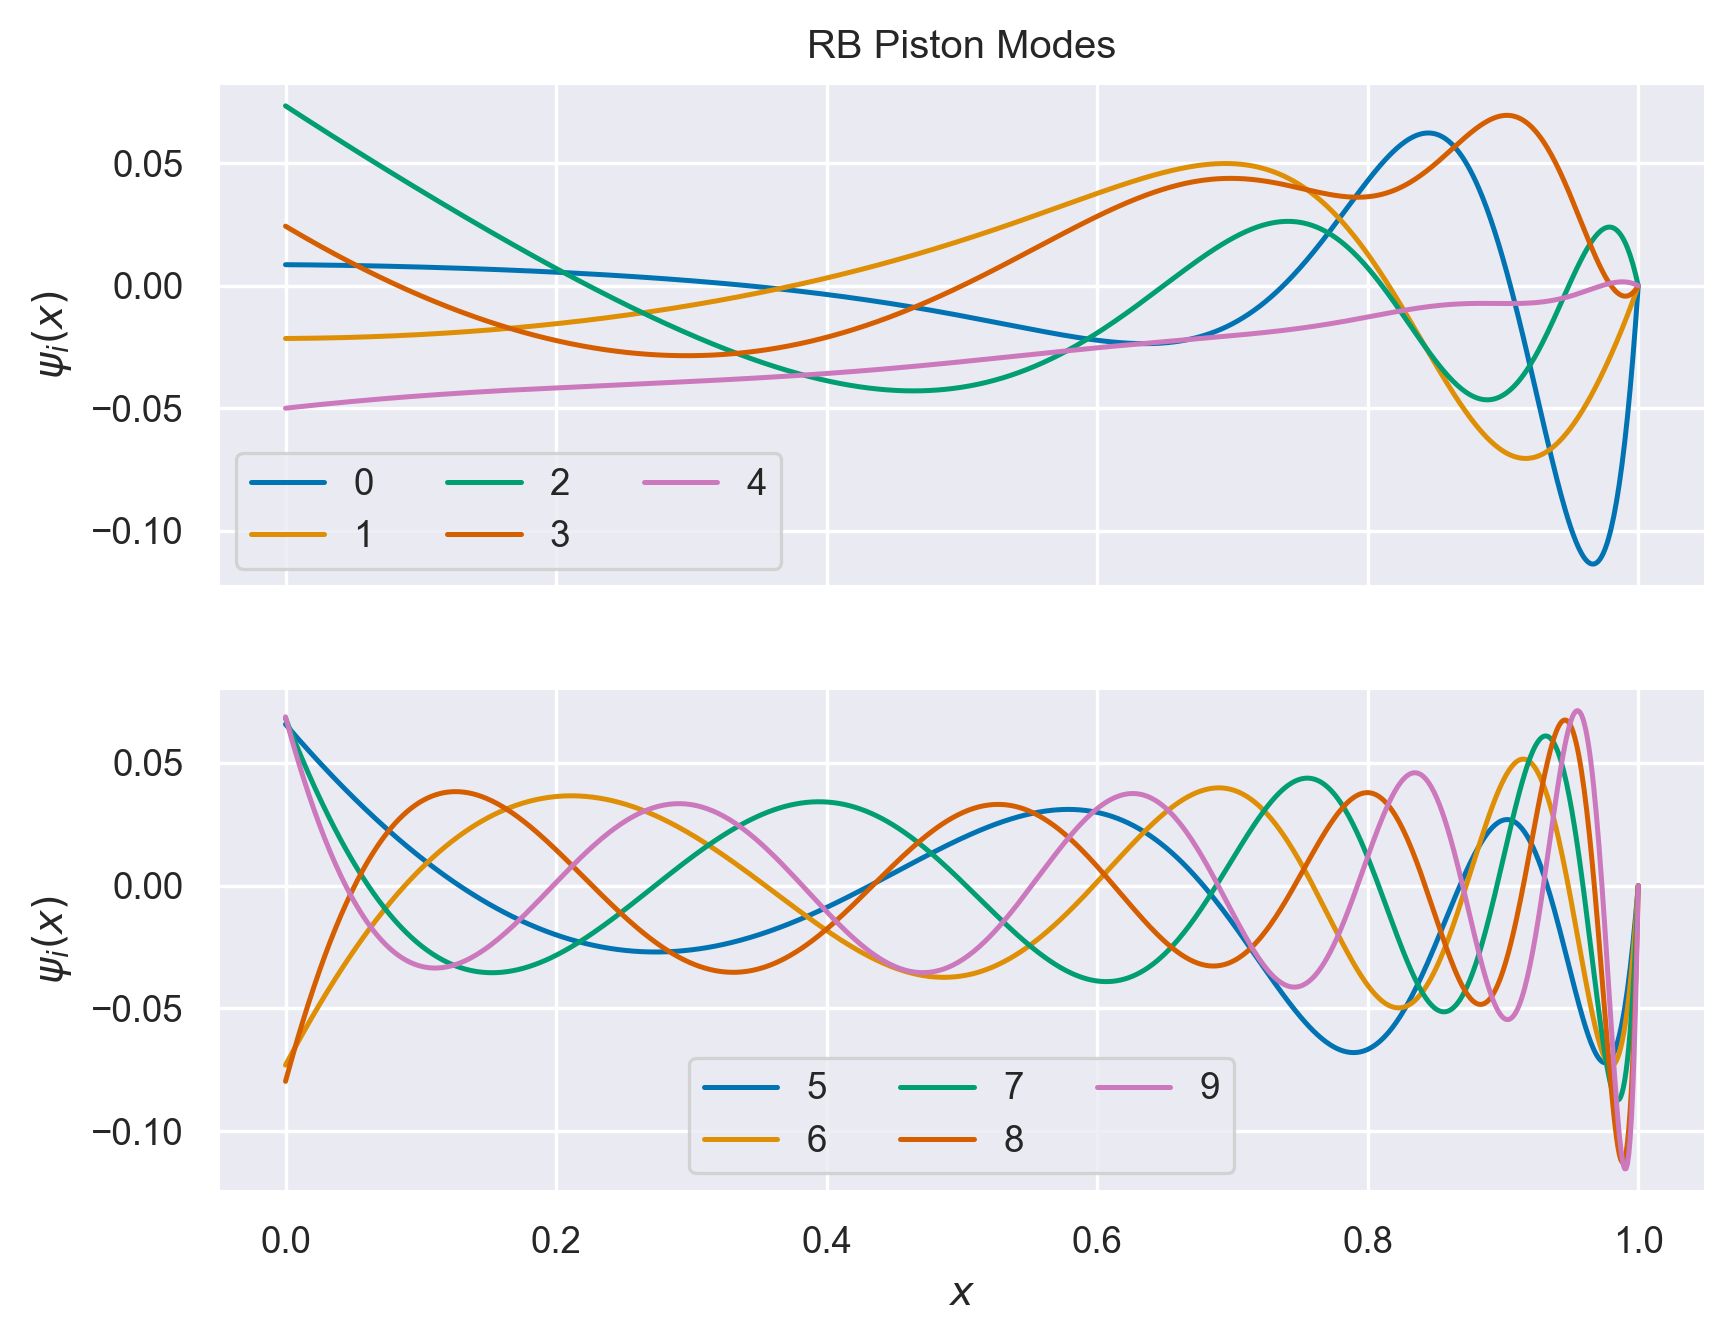
\includegraphics[width=\columnwidth]{research_project/piston/figures/hrom/RB_basis_modes.png}
    \caption{First ten RB solution modes 
    (0-indexing is used to be aligned with code results).
    (Top) First five modes.
    (Bottom) Next five modes.
    The first modes seem to collect the effects of the weak shock wave formation.
    The next five modes look like Fourier modes for different frequencies
    (which is an expected behaviour given the harmonic movement of the piston
    and the sampling for different $\omega$ values during training).
    % since they do not present the piston's harmonic motion
    % (which the remaining modes do seem to collect).
    }
    \label{fig:rb_solution_modes}
\end{figure}

\newpage
\subsection{RB Solution Basis Error}
\label{sec:hrom_results_reduced_basis}
We explore how the number of modes influences the approximation error of the FOM solution.
We have trained our model with 10 random samples according the parameter ranges given in
Tables~\ref{tab:parameter_range} and~\ref{tab:dimensionless_groups}.  
In Table~\ref{tab:uniform_stretching_basis_size} the resulting bases size are reported.
Since the stretching is uniformly spread across the mesh elements, 
despite their change in time,
all the linear operators are trivially reduced.
The RHS requires two RB operator modes because it contains the lifting and its gradient.
\begin{table}[!h]
    \caption{For each operator,
    basis size after the tree walk and final size after tree walk compression.
    The trilinear term and the RB space have the same size, 
    since the RB solution modes were used to evaluated the trilinear term.
    The Nonlinear-lifting operator corresponds to the cross-term lifting matrix
    that arises from the nonlinear convective term.}
    \centering
    \begin{tabular}{@{}rcc@{}}
    \toprule
                      & After Treewalk & Final Size \\ \midrule
    RB                & 295            & 69                \\
    RHS               & 20             & 2                 \\
    Mass              & 10             & 1                 \\
    Stiffness         & 10             & 1                 \\
    Trilinear         & 690            & 69                \\
    Convection        & 20             & 2                 \\
    Nonlinear-lifting & 10             & 1                 \\ \bottomrule
    \end{tabular}
    \label{tab:uniform_stretching_basis_size}
\end{table}
Since we are using the POD to build our reduced basis, 
we attempt to relate POD a posteriori error estimations with 
the actual error between ROM and FOM.

\subsubsection{POD: A Posteriori Errors}
The POD returns a collection of modes and sigular values, 
$(\psi_i(x), \sigma_i)$,
each related to the other.
The magnitude of each singular value $\sigma_i$ somehow encodes 
how much information is carried by its associated mode about the original span.

We define the energy of the basis that contains up to the $i$-th mode as
\begin{equation}
    \mathcal{E}_i = \frac{\sum_{j=0}^{i}\sigma_j^2}{\sum \sigma_k^2}.
\end{equation}
This magnitude is derived from the \textit{a posteriori} error bounds 
for a POD reconstruction, where the following inequality holds,
\begin{equation}
    \norm{y(x) - \sum_{j=0}^{n} w_j \psi_j(x)}_{2}^{2} \leq \sum_{i = n+1}^{N} \sigma_i^2,
\end{equation}
with $y(x)$ belonging to the snapshots used to build the POD basis.
This inequality is telling us that if up to~$n$ basis modes are used
to reconstruct a function belonging to the original span,
the average error in the $L_2$ sense will be smaller or equal
to the sum of the remaining squared singular values.

We shall see if this variable has any predictive power on the ROM error.

\subsubsection{Error Decay}
We want to find the smallest size $N^{*}$ for which the FOM is correctly reproduced.
Naturally, the exact value of this variable is problem-dependent, 
but the way in which we approach its search would suit any RB problem.
\begin{table}[h]
    \centering
    \caption{Online sampling parameters, 
    sorted in ascending order by piston mach~$u_p$ values.}
    \begin{tabular}{cccc}
    \toprule
        $a_0$ & $\omega$ & $\delta$ & $u_p$
        \\ \midrule
        22.96 &   29.55 & 0.15 &           0.20 \\
        19.28 &   22.87 & 0.20 &           0.23 \\
        18.24 &   18.88 & 0.29 &           0.30 \\
        24.64 &   27.13 & 0.29 &           0.32 \\
        20.62 &   25.98 & 0.29 &           0.37
        \\ \bottomrule
    \end{tabular}
\end{table}

In Figure~\ref{fig:error_decay} we present the ROM error with respect to 
the number of RB solution modes and the energy of the truncated basis. 
At this stage, the (M)DEIM approximation is not used
(the FOM operators are projected at each stage).
\begin{figure}[h]
    \centering
    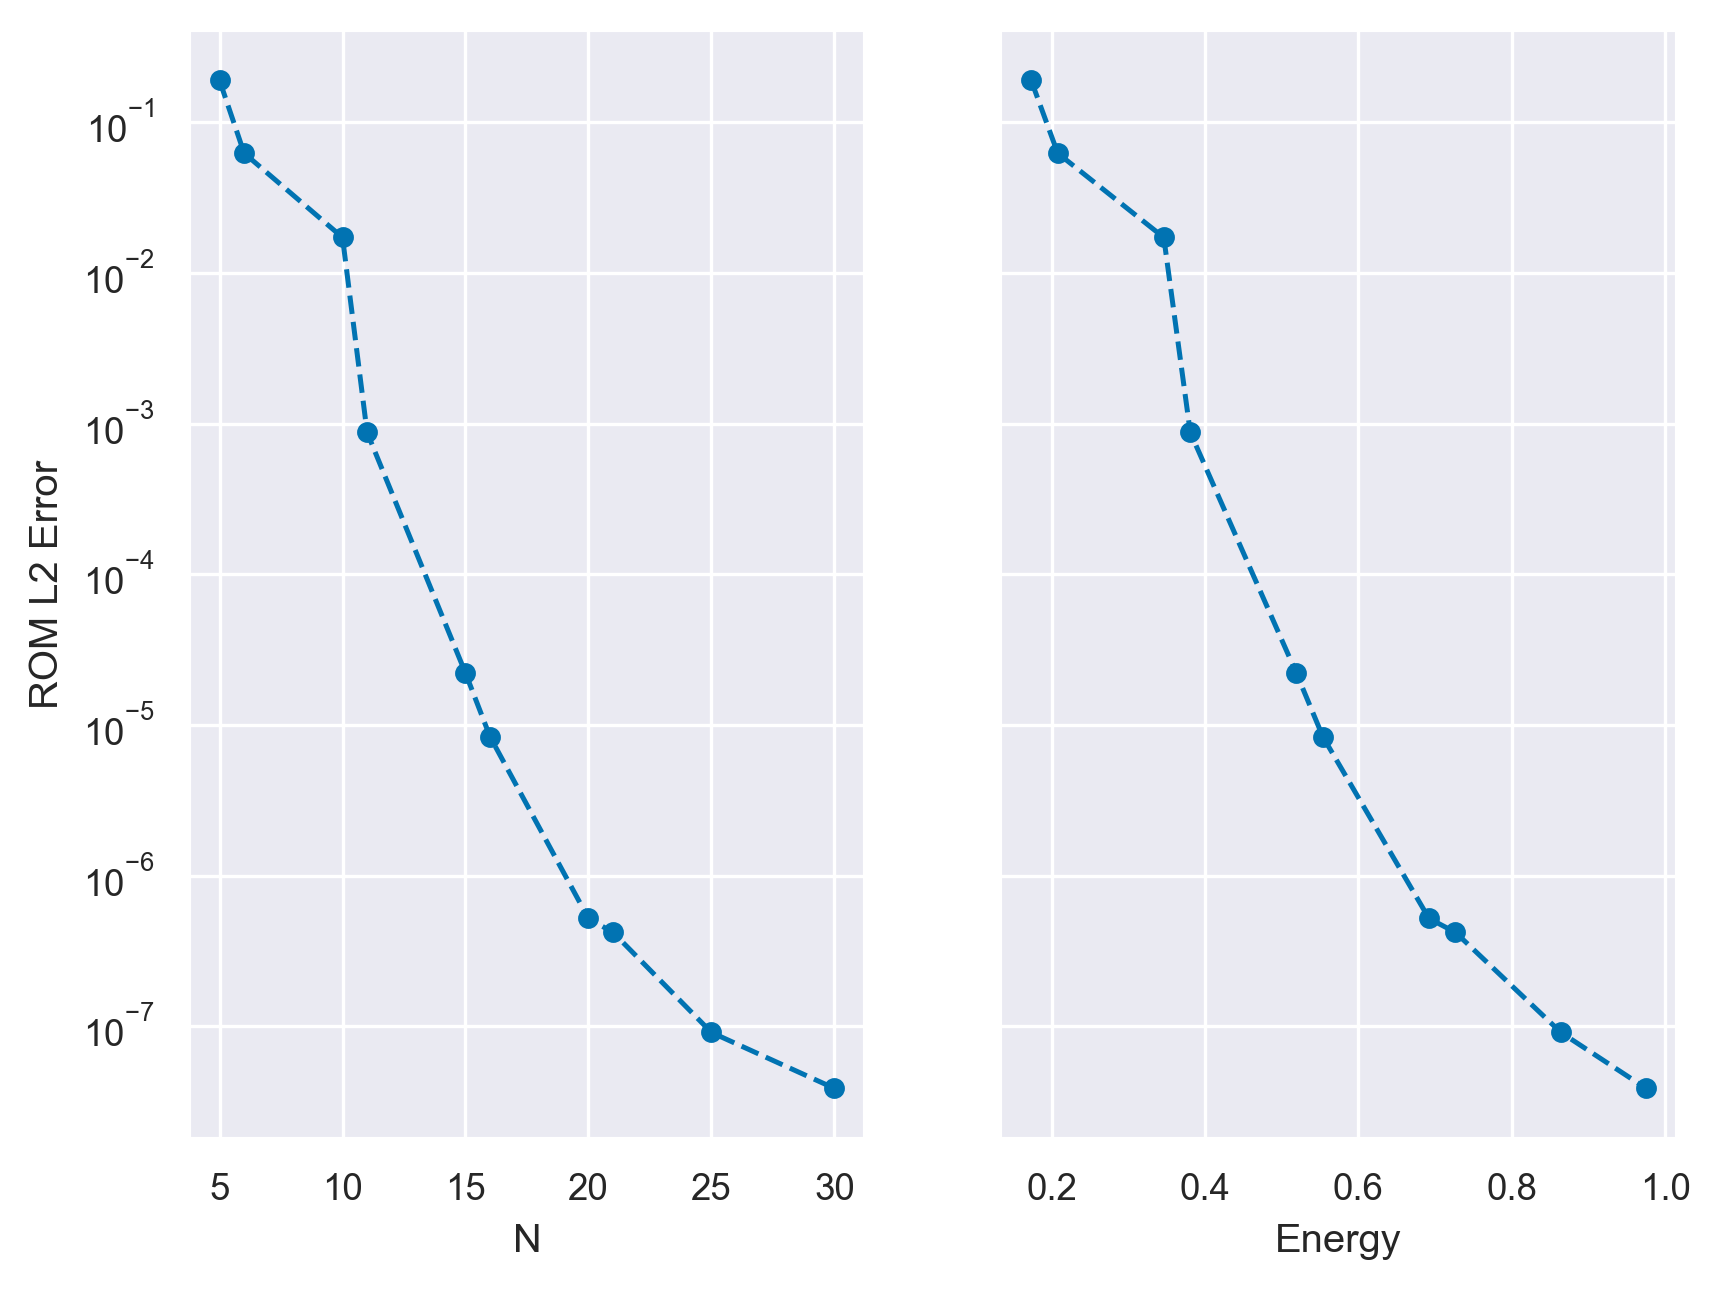
\includegraphics[width=\columnwidth]{research_project/piston/figures/rb_certification/error_decay.png}
    \caption{Error decay vs. the number of RB solution modes and basis energy level.
    Expectedly, the more RB solution modes we have, the lower the error.}
    \label{fig:error_decay}
\end{figure}
The more RB solution modes, the smaller the error.
The more energy the basis contains, the better the approximation.

We present in Figures~\ref{fig:outflow_model_comparison_N_5} 
and \ref{fig:outflow_model_comparison_N_10} 
the actual solution at the outflow for each model (FOM and ROM).
We can see how the ROM model is not accurately resolved for $N=5$, as reflected by the error,
but how it improves for $N=10$.
Clearly, the problem is quite simple to reduce if these few modes are sufficient to reduce the problem.
\begin{figure}[h]
    \centering
    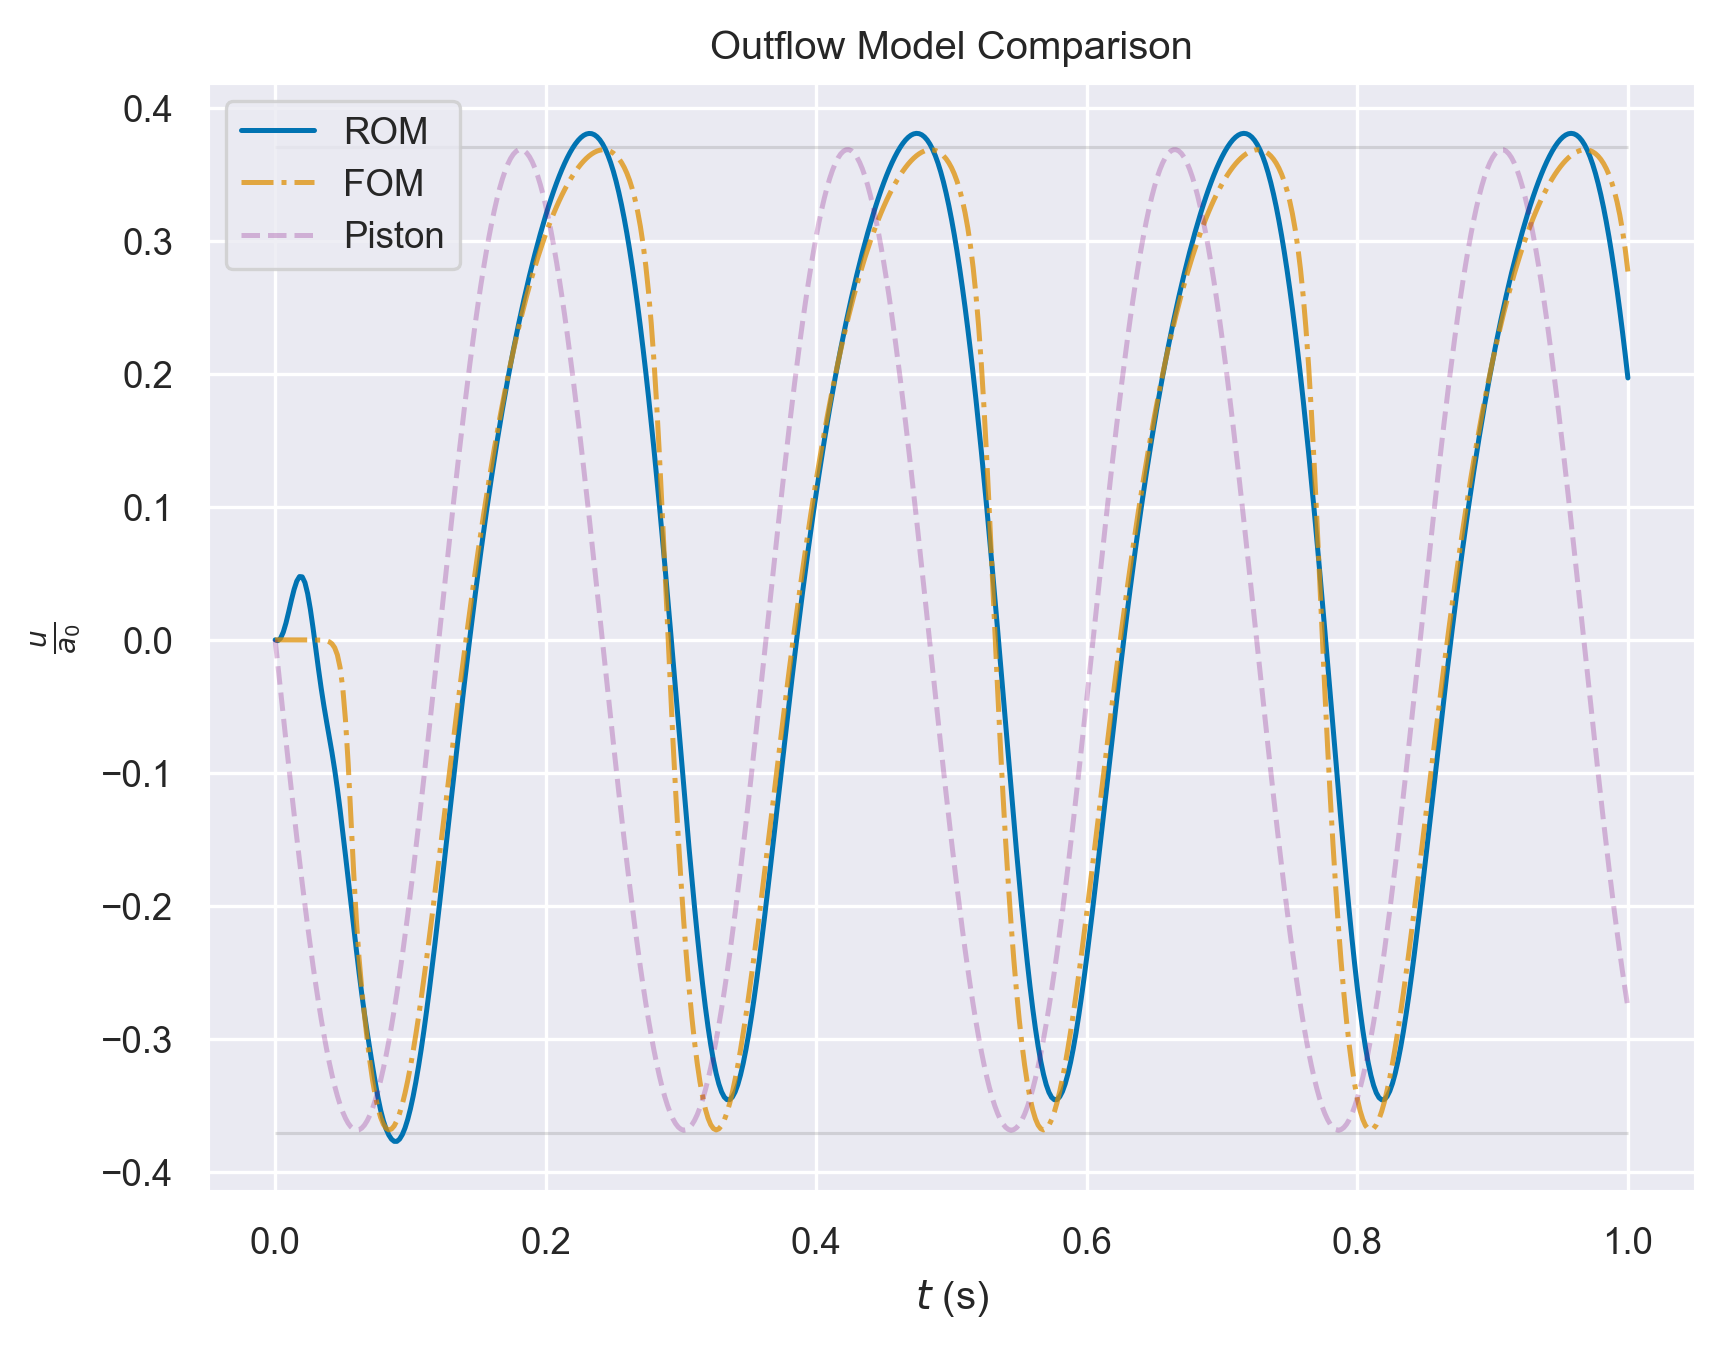
\includegraphics[width=\columnwidth]{research_project/piston/figures/rb_certification/outflow_probes_comparison_rom_5_srom_15_online_4.png}
    \caption{Outflow velocities for different models, for $N=5$ RB solution modes. 
    It is inaccurately resolved at the beginning of the transient 
    and some difussion is introduced, reducing the extrema values.}
    \label{fig:outflow_model_comparison_N_5}
\end{figure}
\begin{figure}[h]
    \centering
    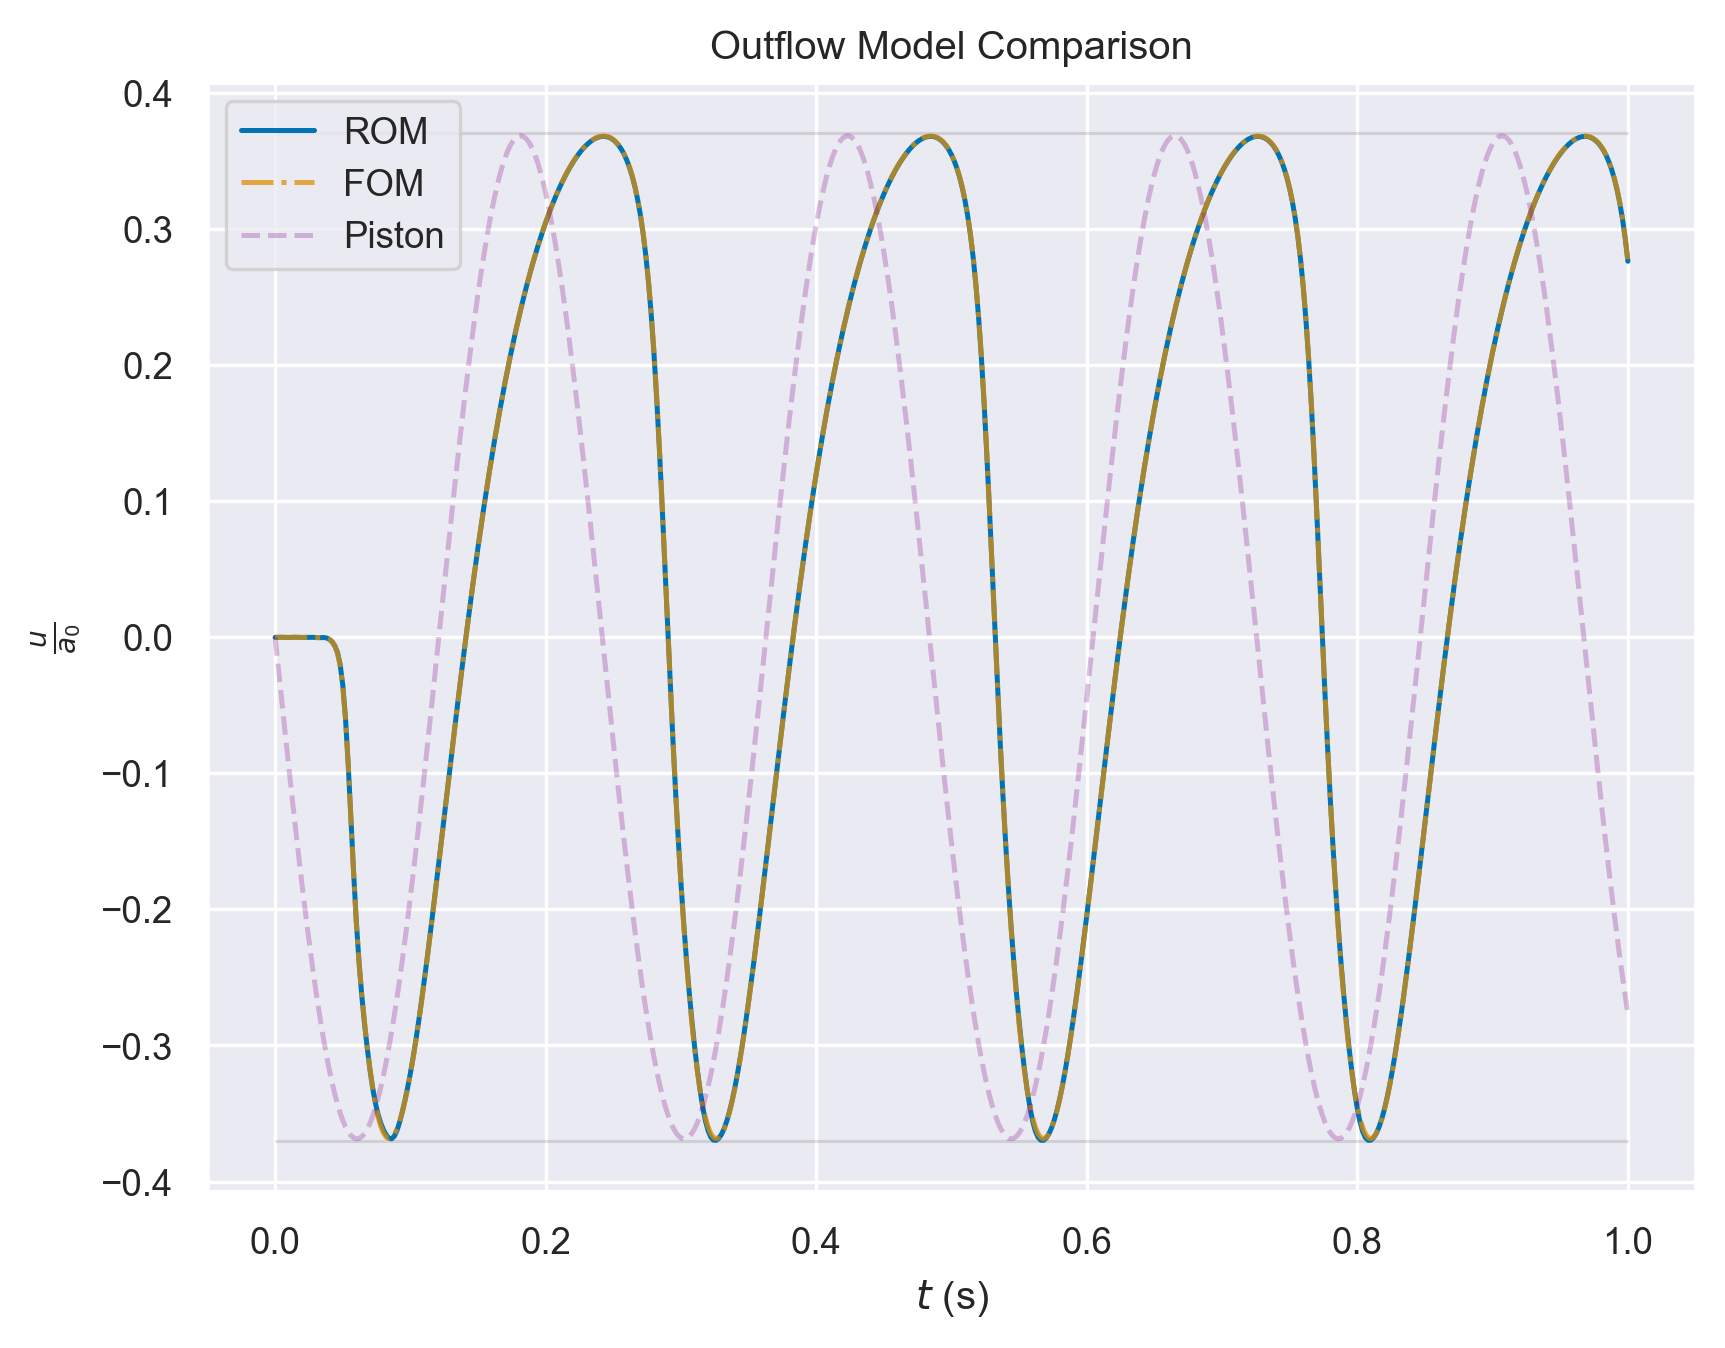
\includegraphics[width=\columnwidth]{research_project/piston/figures/rb_certification/outflow_probes_comparison_rom_10_srom_20_online_4.png}
    \caption{Outflow velocities for different models. 
    The ROM model is better resolved for $N=10$ RB solution modes.}
    \label{fig:outflow_model_comparison_N_10}
\end{figure}
The flow departs from rest as the piston starts to move.
Therefore, the first snapshots contain a nonlinearity in the sense that the flow starts to move on one side, 
but remains still along the rest of the tube.

However, for most of the time interval, 
this kind of nonlinearity is not present again,
since the flow is in constant motion, flowing in and out of the system.
Hence, it is an expected behaviour that for the initial interval the ROM is inaccurate,
unless we include a sufficient number of RB solution modes.
To fix this problem, certain techniques exist which enhance the POD basis 
without adding excessive complexity \cite{weightedPOD}.

% \newpage
\subsection{N-MDEIM Basis Error}
\label{sec:uniform_mdeim_errors}
In this section we explore the reduction of the trilinear operator
for the mesh with uniform stretching.

In Section~\ref{sec:us_hierarchical_basis} we present the results for
the basis resulting from the snapshots collected from the FOM simulation.
In Section~\ref{sec:reduced_basis_mdeim_error_interaction} we investigate
the interaction between the RB and MDEIM errors.
Finally, in Section~\ref{sec:us_non-hierarchical_basis} we present the results for
the snapshots resulting from the snapshots collected from RB mode evaluation
in the trilinear form.

We refer to the collateral basis of the trilinear operator as the N-MDEIM basis.

\subsubsection{N-MDEIM: Hierarchical Basis}
\label{sec:us_hierarchical_basis}
We present the results for the \mbox{$u^{*}$-general} strategy,
for the uniform stretching mesh displacement.
During the simulation of the FOM, 
we collect snapshots of the trilinear term and compress them with the same  
nested POD strategy as we did for the reduced basis, 
Section~\ref{sec:1d_rom_burgers_basis_construction_nested}.

By doing so, we obtain a hierarchical basis, which allows us to tune the error,
as proved by the singular value decay (Figure~\ref{fig:sigmas_decay_from_fom}).
The singular value decay for the trilinear operator presents the same pattern 
as the one for the solution.
% This has to do with the fact that this operator is a trilinear form.
The reduction difficulty is the same as the one
required for the reduced basis.
\begin{figure}[h]
    \centering
    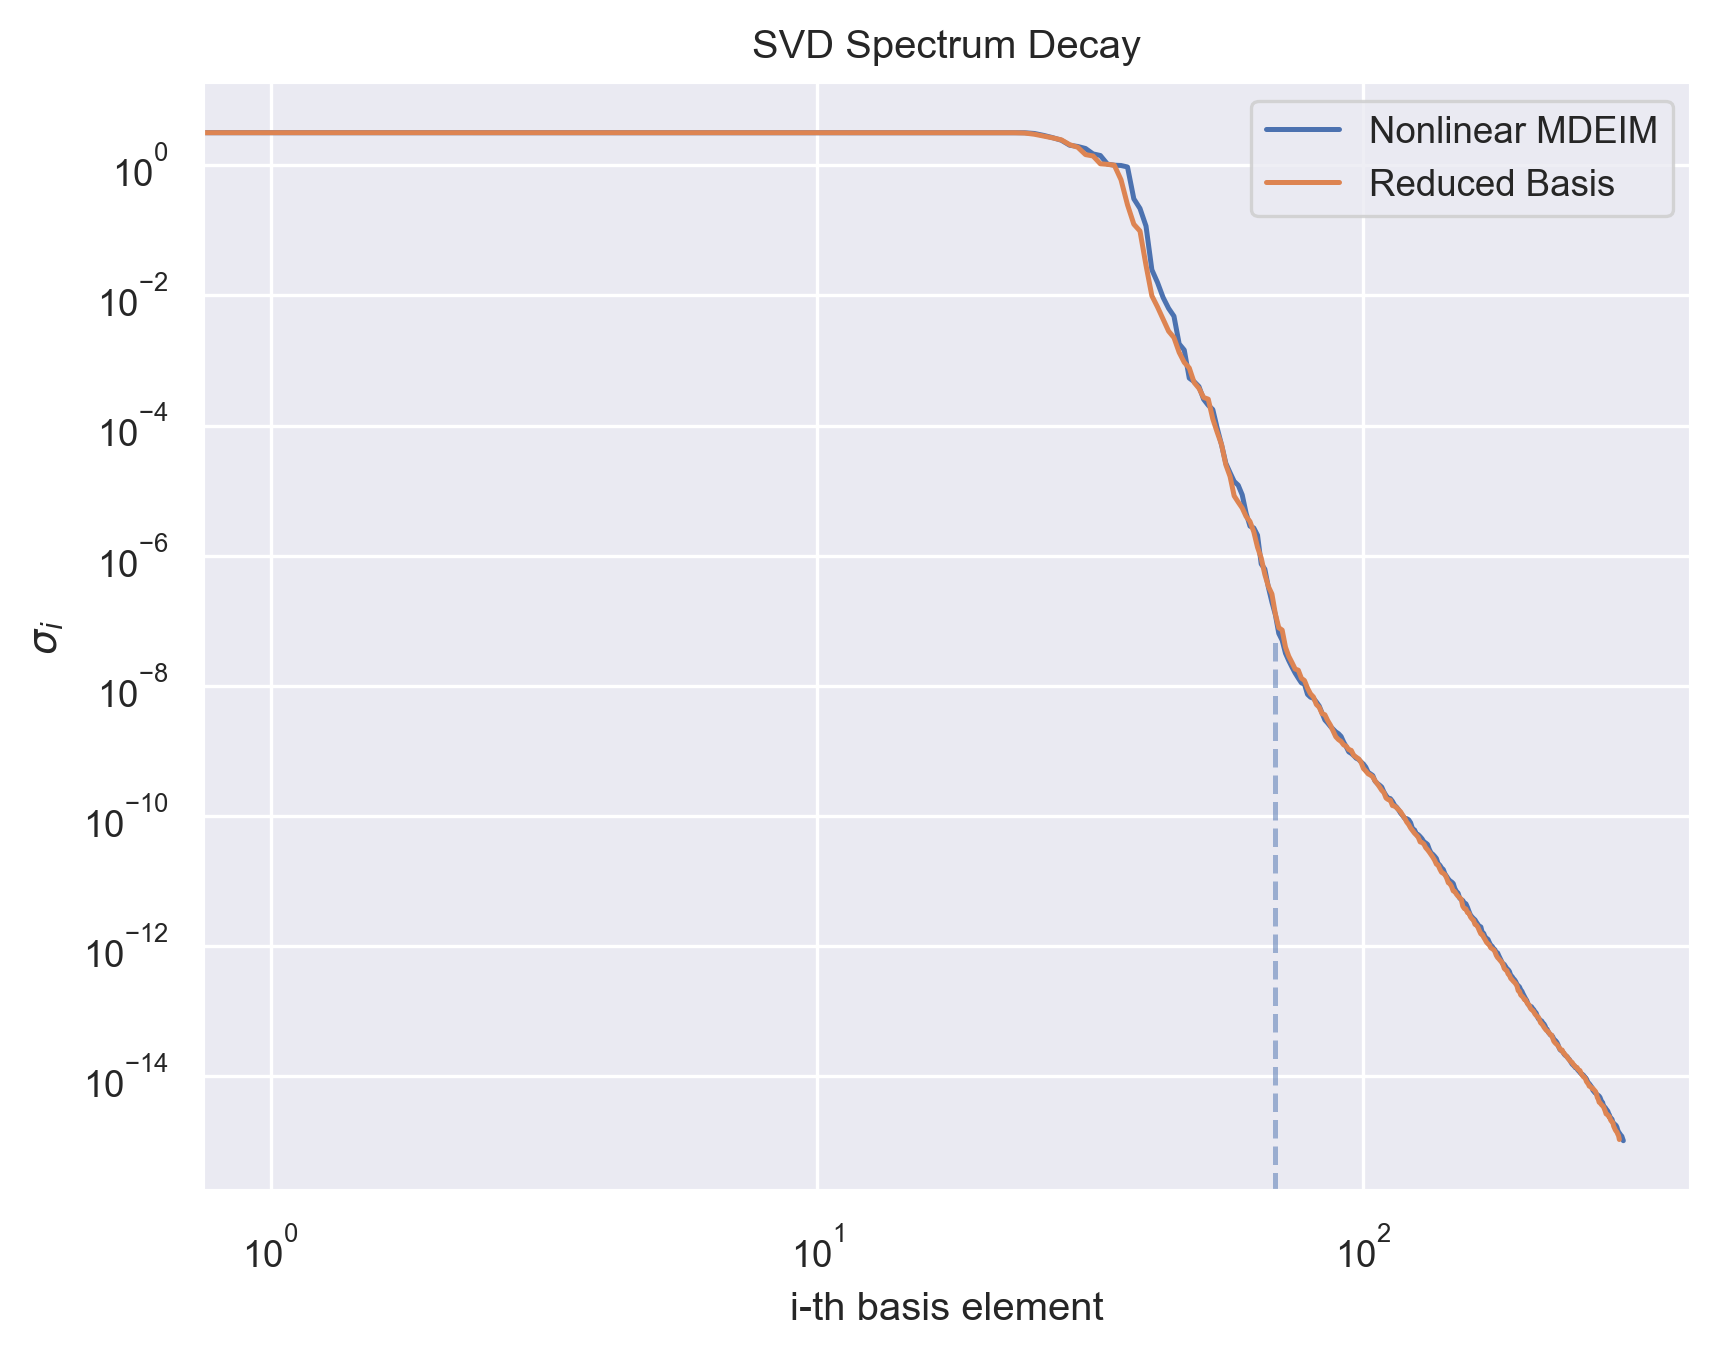
\includegraphics[width=1\columnwidth]{research_project/piston/figures/mdeim_certification/sigmas_problem_from_fom.png}
    \caption{Singular values decay for the reduced basis and the trilinear operator.
    The dashed vertical line corresponds to the number of modes, $N=69$.
    The basis for the trilinear operator presents the same pattern 
    (and hence the same size)
    as the solution reduced basis.
    This is due to the fact that the operator is a trilinear form.
    Hence, due to the simplicity of the Jacobian, the reduction difficulty is similar to the one
    required for the reduced basis.}
    \label{fig:sigmas_decay_from_fom}
\end{figure}

In Table~\ref{tab:mdeim_certification} we show the parameter range for which
we tested this basis against the first ten modes.
\begin{table}[h]
    \centering
    \caption{Parameter space sampling for trilinear term reconstruction.}
    \label{tab:mdeim_certification}
    \begin{tabular}{cccc}
        \toprule
        $a_0$  & $\omega$ & $\delta$ & $u_p$ \\
        \midrule
        24.275 &  18.549  & 0.203 &  0.155 \\
        21.055 &  15.969  & 0.236 &  0.179 \\
        23.627 &  24.427  & 0.211 &  0.218 \\
        21.533 &  24.376  & 0.200 &  0.226 \\
        20.440 &  18.913  & 0.289 &  0.267 \\
        23.849 &  27.396  & 0.261 &  0.300 \\
        19.976 &  23.190  & 0.259 &  0.301 \\
        20.633 &  24.184  & 0.280 &  0.329 \\
        18.803 &  29.705  & 0.226 &  0.357 \\
        19.890 &  27.986  & 0.278 &  0.391 \\
        \bottomrule
\end{tabular}
\end{table}
In Figure~\ref{fig:nonlinear_error_decay_from_fom_by_parameter} 
% and~\ref{fig:nonlinear_error_decay_from_fom}
we present the reconstruction error decay, as the N-MDEIM basis is truncated.
The basis shows the expected error decay as modes are removed,
hence allowing to speed up even further computations 
if some compromise is made in the error.

\begin{figure}[h]
    \centering
    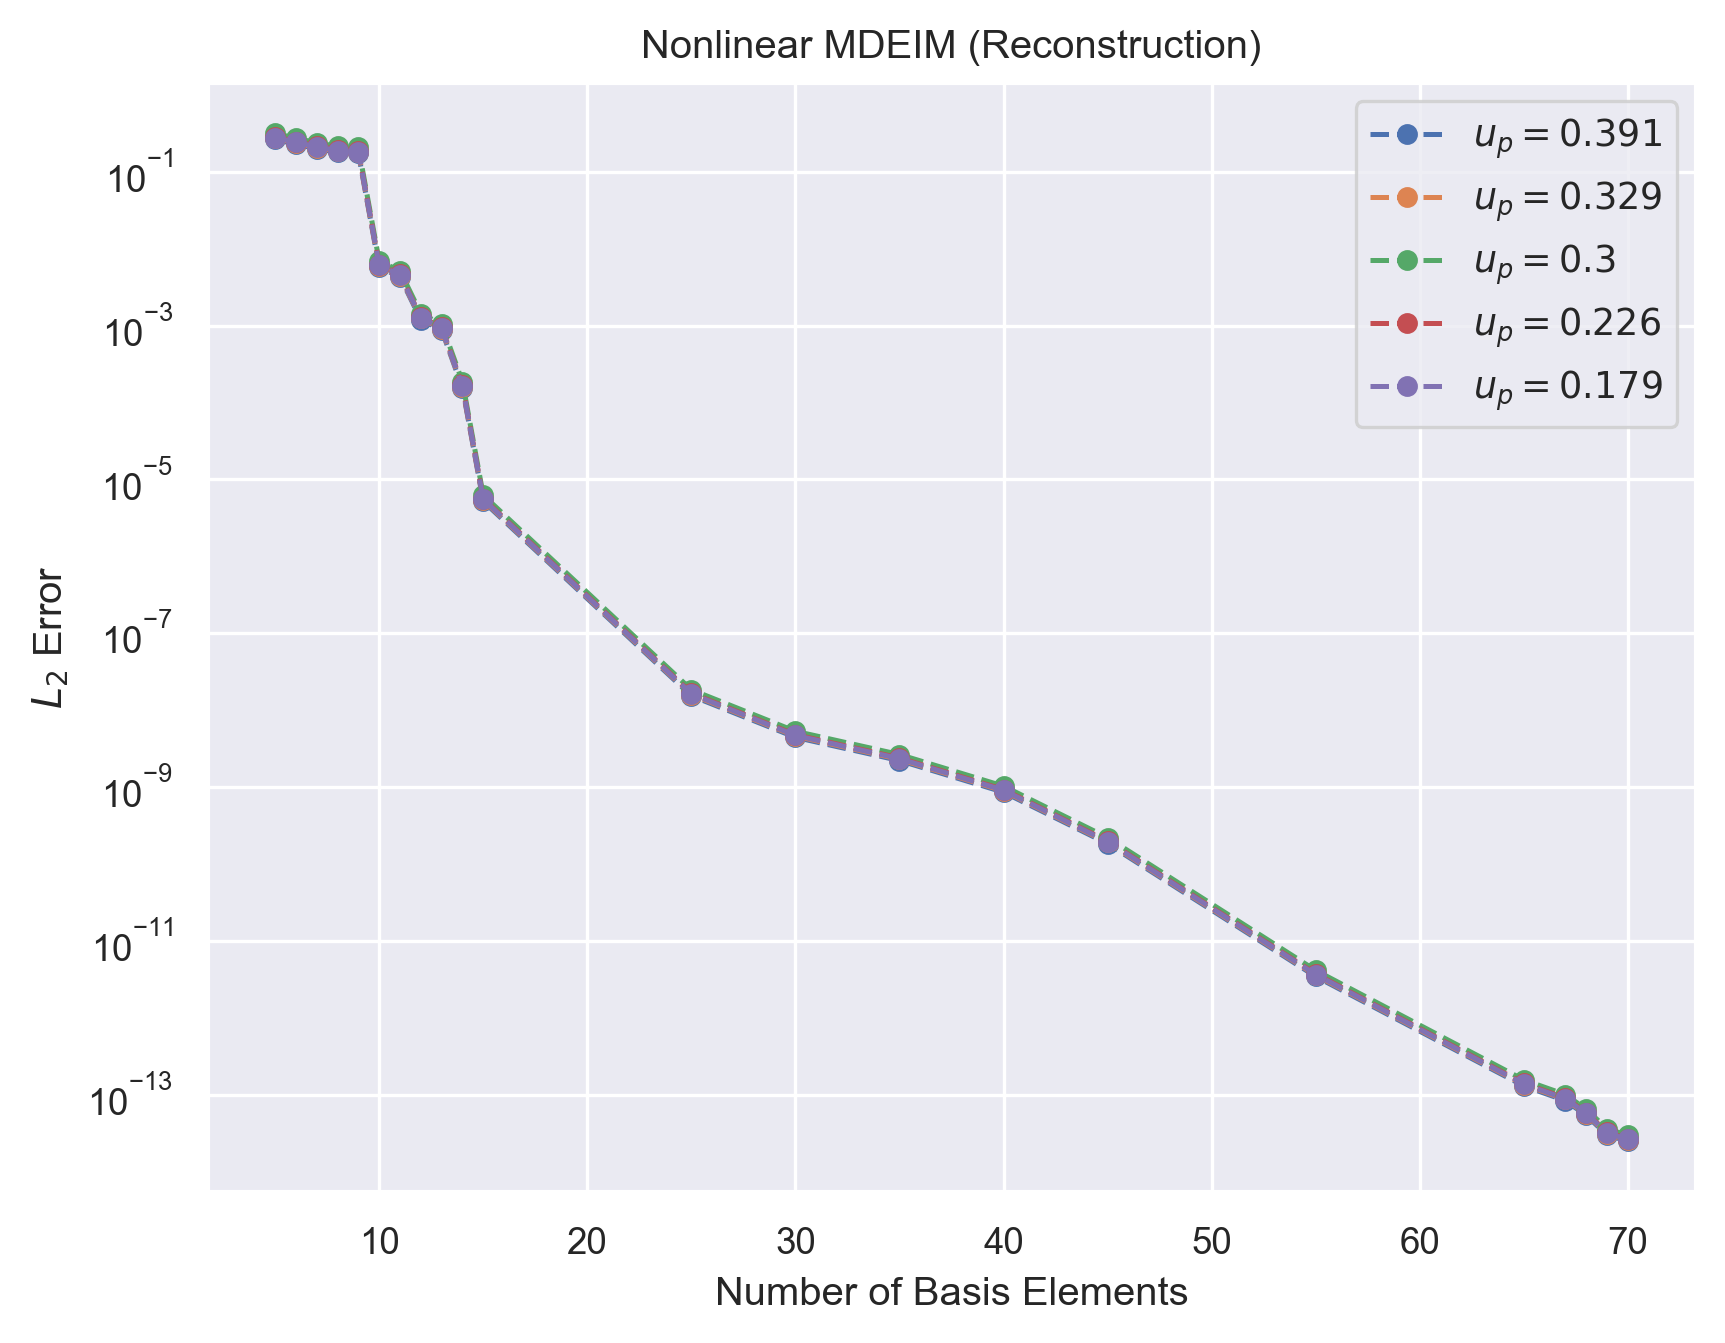
\includegraphics[width=1\columnwidth]{research_project/piston/figures/mdeim_certification/nonlinear_error_decay_by_parameter.png}
    \caption{N-MDEIM reconstruction error decay, 
    as we truncate the modes from the MDEIM basis for some individual parametrizations.
    Due to the simplicity of the problem, 
    the (implicit) Jacobian and 
    the fact that the linearized term is trilinear in all of its arguments, 
    there is no noticeable difference for different parametrizations.}
    \label{fig:nonlinear_error_decay_from_fom_by_parameter}
\end{figure}

% \begin{figure}[h]
%     \centering
%     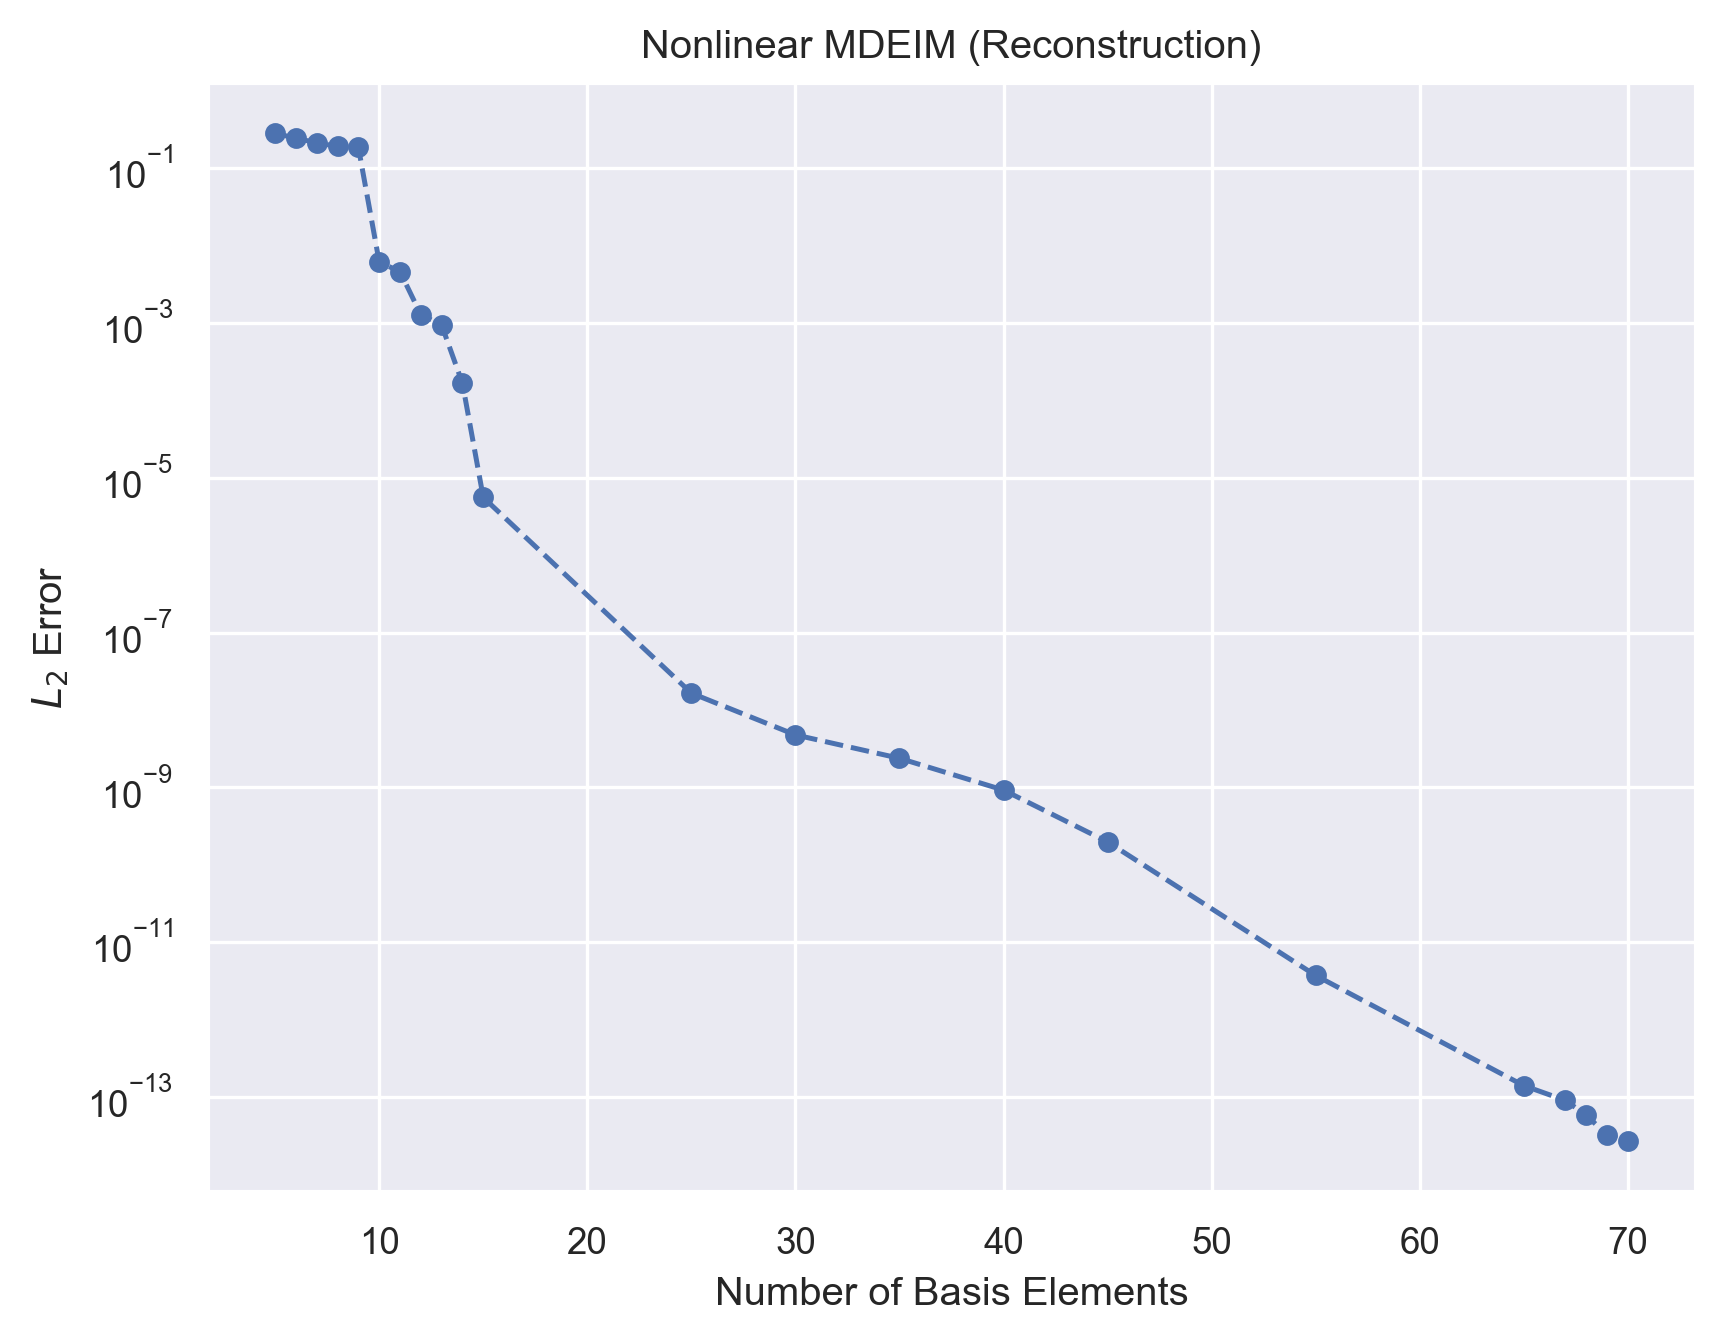
\includegraphics[width=1\columnwidth]{research_project/piston/figures/mdeim_certification/nonlinear_error_decay_from_fom.png}
%     \caption{N-MDEIM reconstruction error decay, 
%     as we truncate the modes from the MDEIM basis, averaged across parametrizations.}
%     \label{fig:nonlinear_error_decay_from_fom}
% \end{figure}

\subsubsection{RB and N-MDEIM Error Interaction}
\label{sec:reduced_basis_mdeim_error_interaction}
With two bases (solution and trilinear operator) which show error decay, 
we can truncate them simultaneously, 
to determine their interaction.
In Table~\ref{tab:nonlinear_error_decay_heatmap} we present 
the timewise $L_2$ error for different numbers of RB solution 
and RB trilinear modes.
In Figure~\ref{fig:nonlinear_error_decay_heatmap} we present the same table,
albeit in a heatmap plot. 

Expectedly, we reach a situation where one error dominates the other one.
Increasing the size of one basis will not improve the
results, unless the other one is enlarged too.
If we wanted to achieve a determined error threshold,
we would have to analyze and take into account both bases errors simultaneously.
\begin{table}[h]
    \centering
    \caption{Timewise $L_2$ error decay for different truncation levels 
    of the reduced basis space (N) 
    and the trilinear operator basis (N-MDEIM).}
    \begin{tabular}{ccccccc}
        \toprule
        N-MDEIM &      5  &      10 &      15 &      30 &      40 &      50 \\
        N  &         &         &         &         &         &         \\
        \midrule
        5  & 3.4e-2 & 3.4e-2 & 3.4e-2 & 3.4e-2 & 3.4e-2 & 3.4e-2 \\
        10 & 3.4e-3 & 7.8e-4 & 7.8e-4 & 7.8e-4 & 7.8e-4 & 7.8e-4 \\
        15 & 3.3e-3 & 2.1e-5 & 1.4e-5 & 1.4e-5 & 1.4e-5 & 1.4e-5 \\
        20 & 3.3e-3 & 1.7e-5 & 8.0e-7 & 7.8e-7 & 7.8e-7 & 7.8e-7 \\
        25 & 3.3e-3 & 1.7e-5 & 2.8e-7 & 1.5e-7 & 1.5e-7 & 1.5e-7 \\
        30 & 3.3e-3 & 1.7e-5 & 2.5e-7 & 5.1e-8 & 5.3e-8 & 5.3e-8 \\
        35 & 3.3e-3 & 1.7e-5 & 2.5e-7 & 4.5e-8 & 4.6e-8 & 4.6e-8 \\
        \bottomrule
    \end{tabular}
    \label{tab:nonlinear_error_decay_heatmap}
\end{table}

\begin{figure}
    \centering
    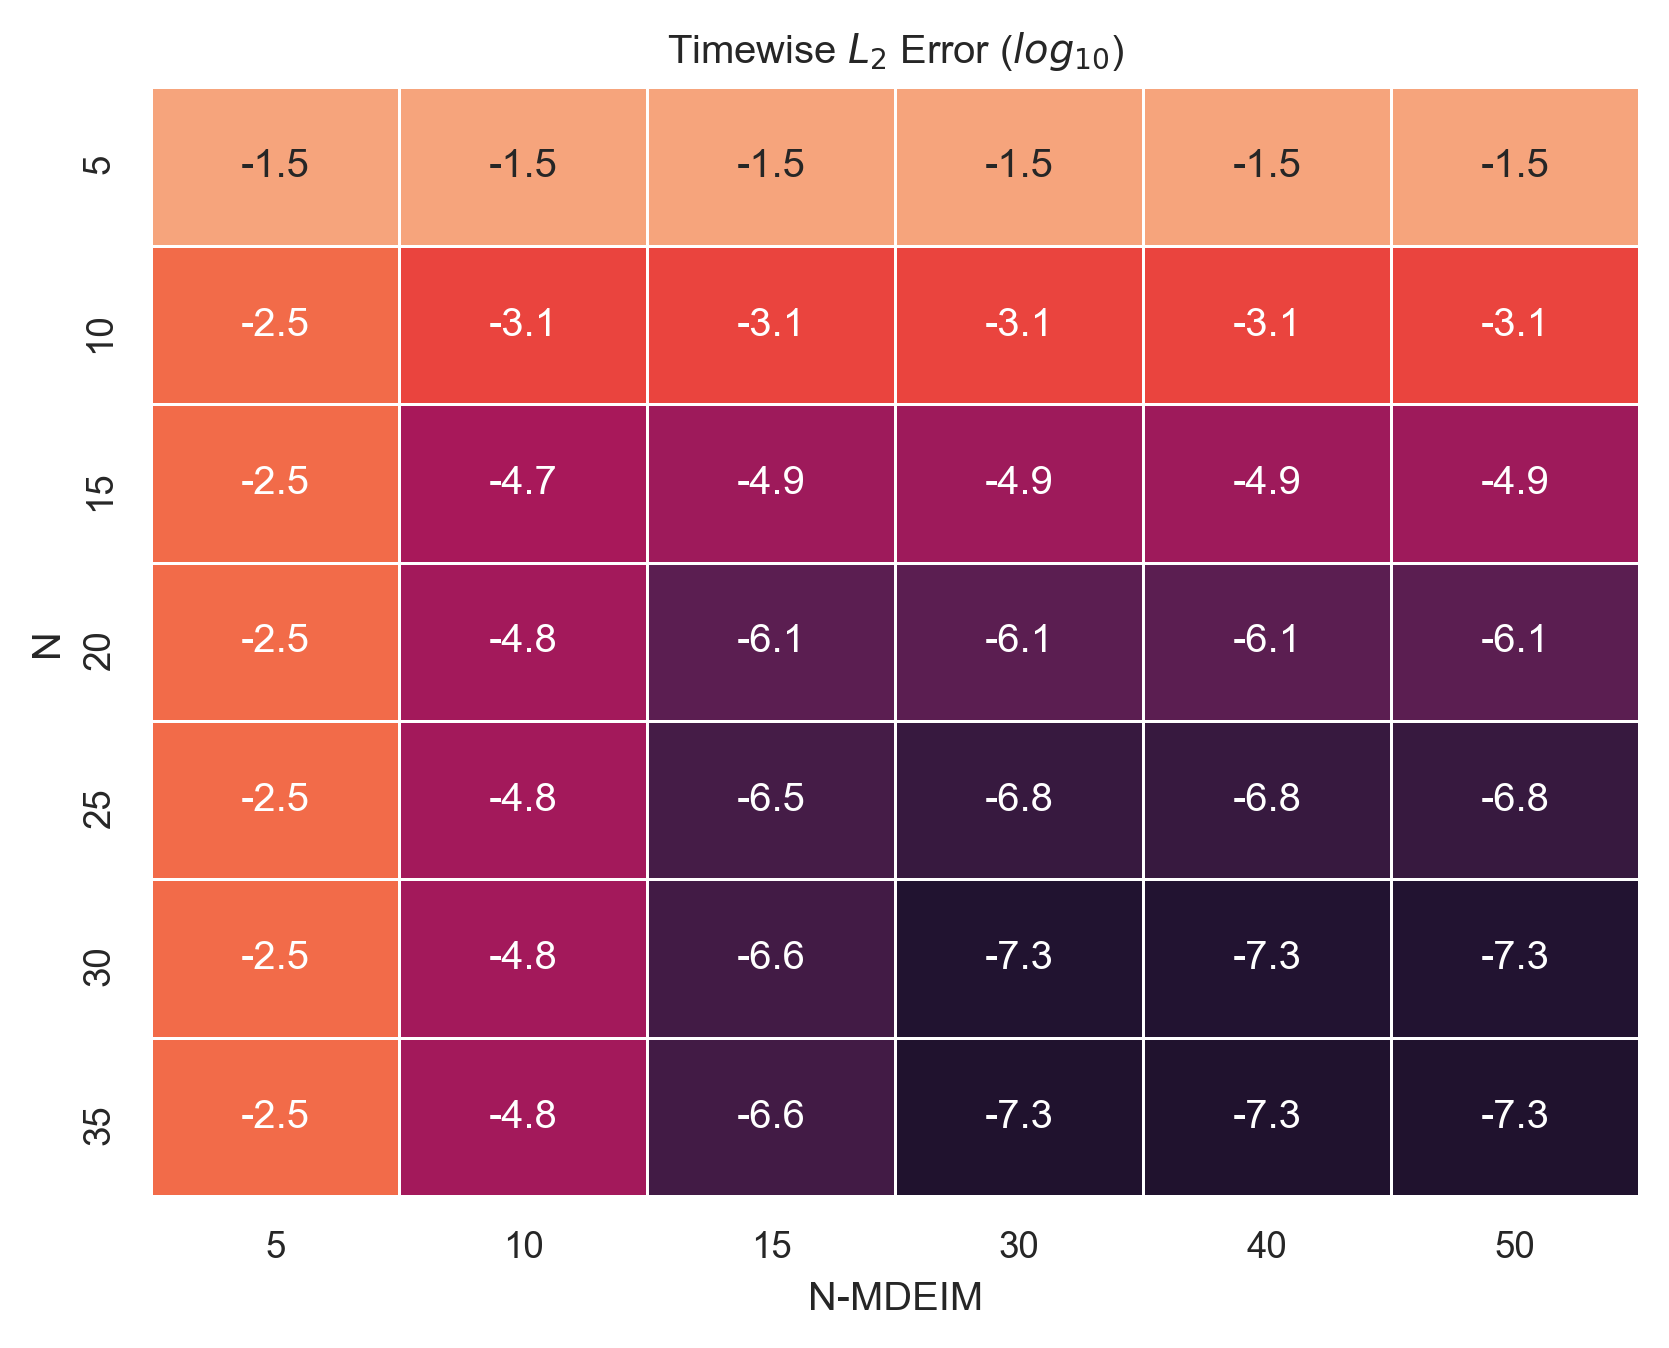
\includegraphics[width=1\columnwidth]{research_project/piston/figures/mdeim_certification/error_decay_heatmap.png}
    \caption{Timewise $L_2$ error decay for different truncation levels 
    of the reduced basis space (N) 
    and the trilinear operator basis (N-MDEIM).
    The $log_{10}$ transformation was applied, so that the heatmap color gradient is smooth.}
    \label{fig:nonlinear_error_decay_heatmap}
\end{figure}

\subsubsection{N-MDEIM: Non-Hierarchical Basis}
\label{sec:us_non-hierarchical_basis}
Now we see what happens if we build the MDEIM basis 
from trilinear snapshots assembled with RB solution modes 
($u^{*}$-restricted).

The first ten RB solution modes are used to assemble the operator for the ten parameters
from Table~\ref{tab:mdeim_certification}.
In Figure~\ref{fig:mdeim_error_approximation} we show the mean approximation error
in time for the trilinear operator on these same RB solution modes. 
We see that unless the complete basis is used ($N=69$),
the approximation error is quite poor.
\begin{figure}[h]
    \centering
    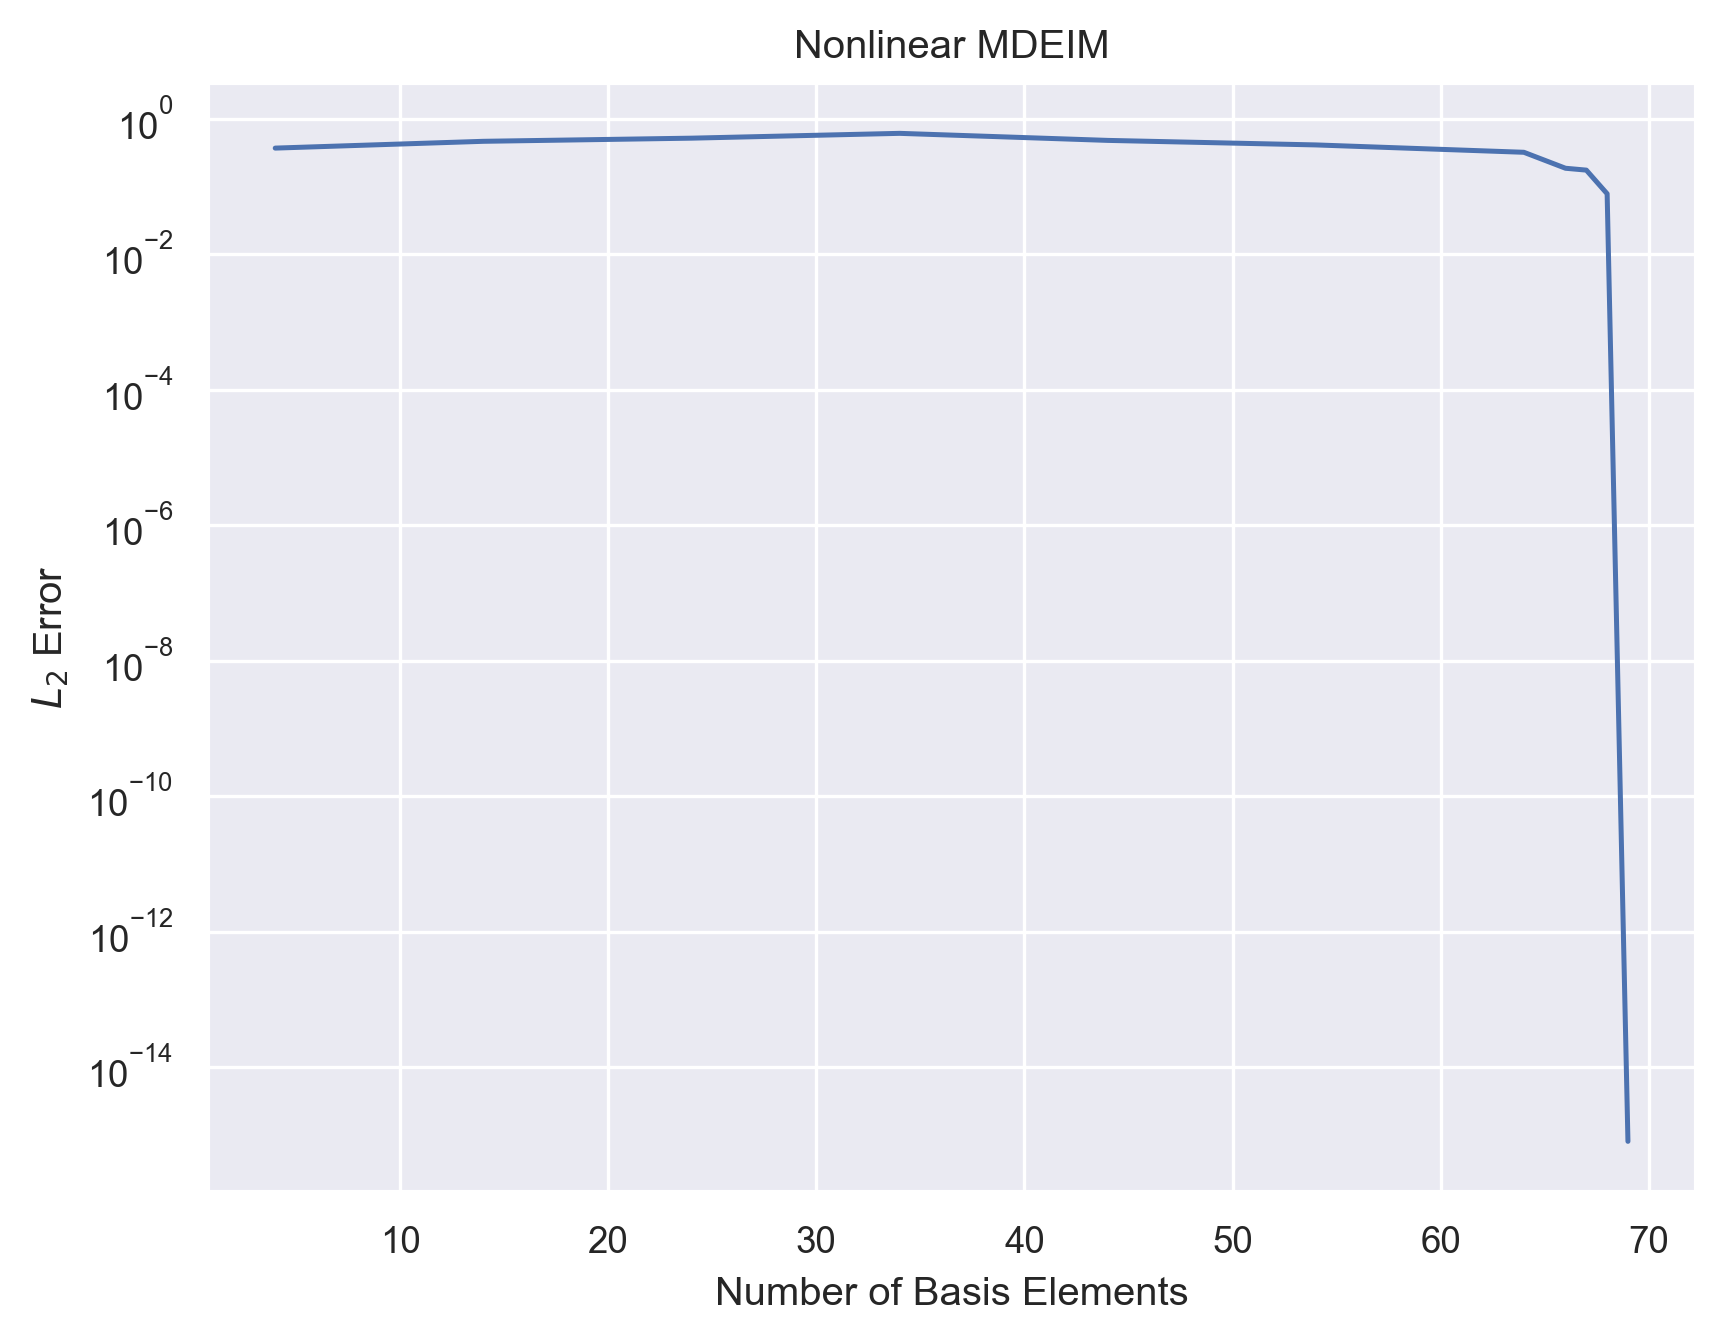
\includegraphics[width=1\columnwidth]{research_project/piston/figures/mdeim_certification/nonlinear_error_decay.png}
    \caption{N-MDEIM error approximation on the first ten RB solution modes 
    for different collateral basis size.
    The first ten RB solution modes were used to assemble the operator.
    The approximation is quite poor, unless the complete basis is used 
    ($N=69$).}
    \label{fig:mdeim_error_approximation}
\end{figure}

This has to do with the fact that the RB solution modes,
which form an orthogonal basis, were used to assemble the trilinear operator snapshots.
Hence, all the result RB operator modes contain fundamental information,
as hinted by the abrupt drop in the singular value, see Figure~\ref{fig:sigmas_decay}. 
\begin{figure}
    \centering
    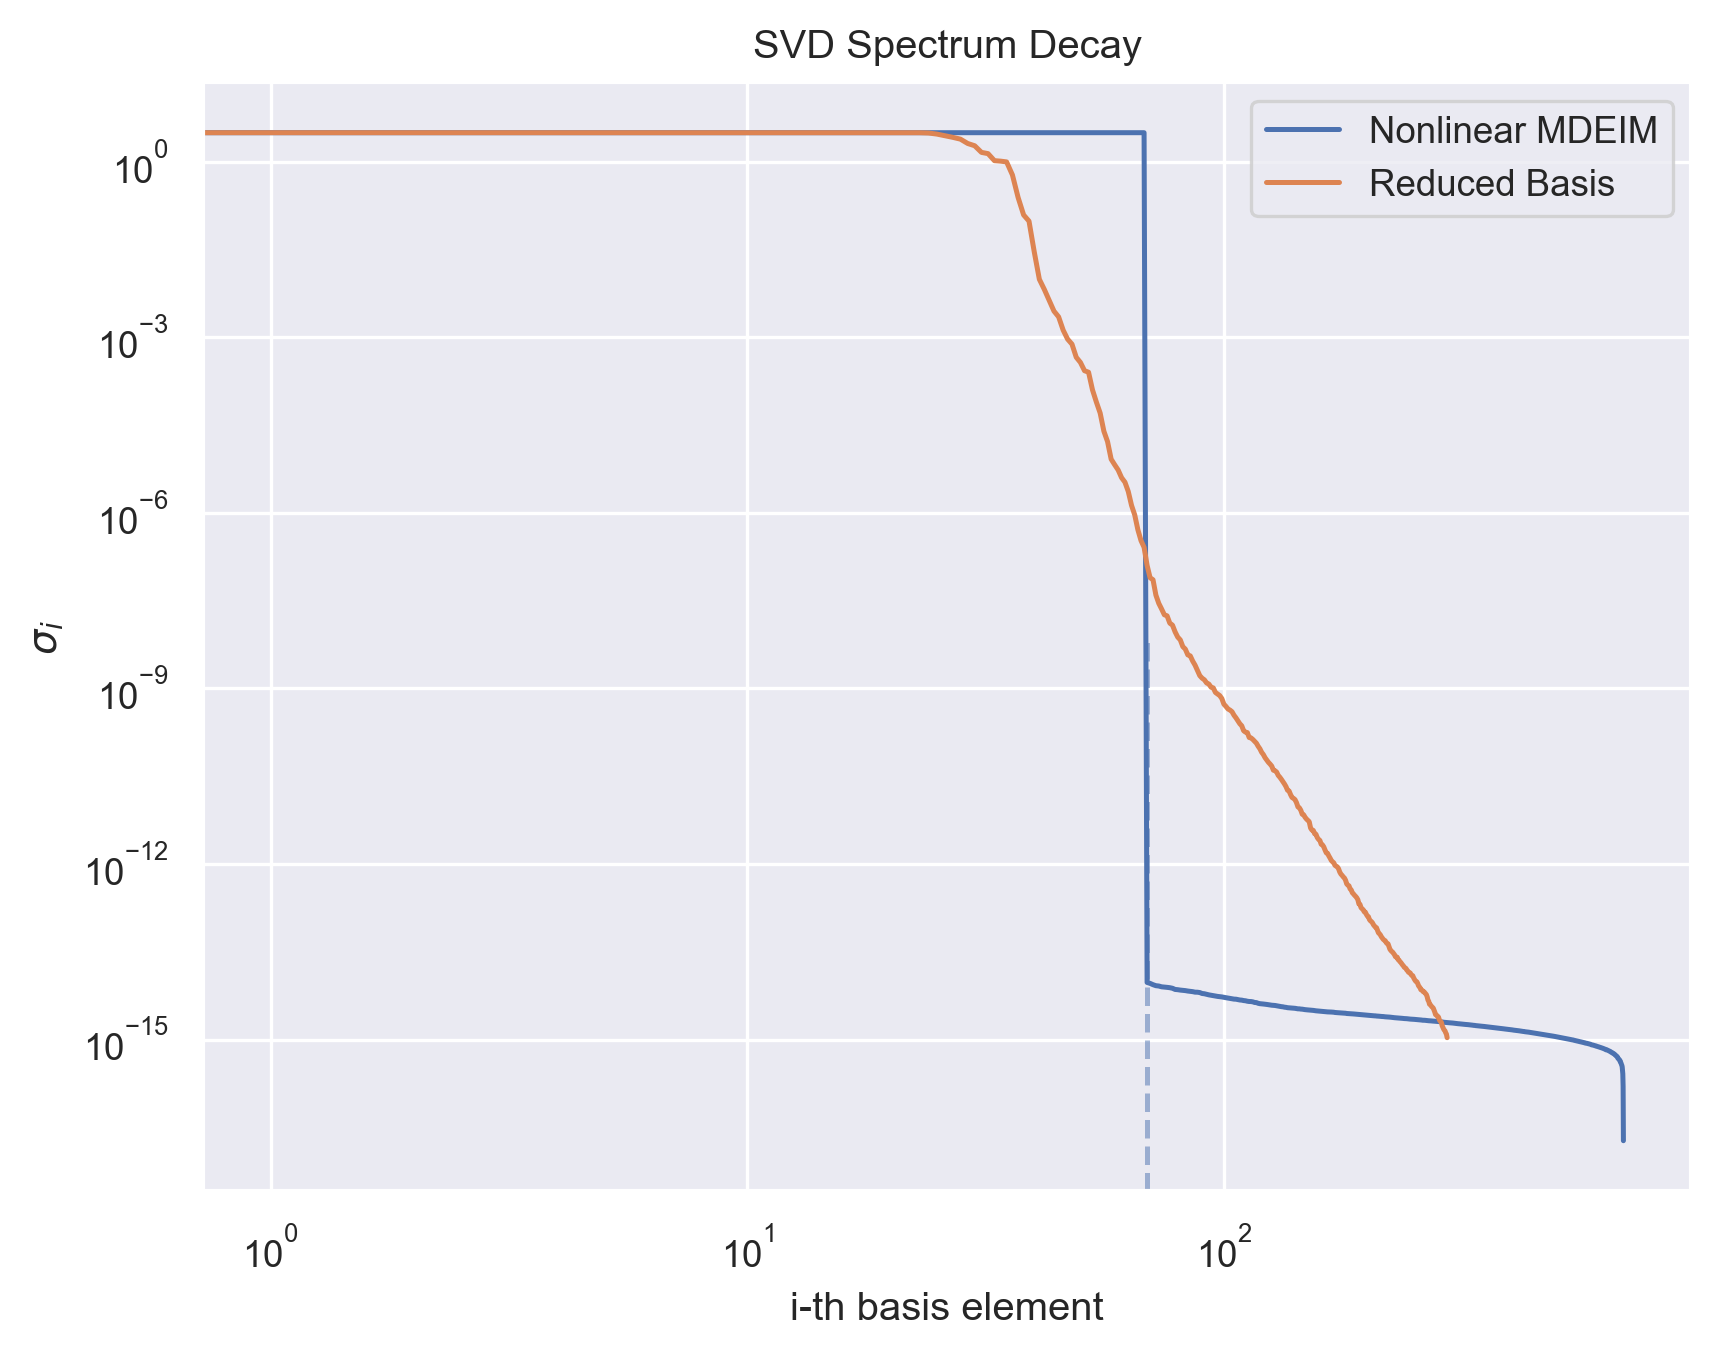
\includegraphics[width=1\columnwidth]{research_project/piston/figures/mdeim_certification/sigmas_problem.png}
    \caption{Singular values decay for the reduced basis and the trilinear operator.
    The dashed vertical line corresponds to the number of reduced modes, $N=69$.
    The singular value decay for the trilinear operator does 
    not present the same pattern as the one for the reduced basis.
    All RB trilinear operator modes 
    seem to contain the same amount of information from the original span.
    This has to do with the fact that the modes,
    which form an orthogonal basis, 
    were used to assemble the trilinear operator snapshots.}
    \label{fig:sigmas_decay}
\end{figure}
We have obtained a basis that allows us to reduce the assembly of the operator, 
but it doesn't allow us to tune the error.
We name such basis \textit{non-hierarchical}, 
because there is no decay in its singular value spectrum.
We will clarify the loss of hierarchy in Section~\ref{sec:nonhierachical_pod_bases}.

\newpage
\subsection{Non-Hierachical POD Bases}
\label{sec:nonhierachical_pod_bases}
We investigate further the non-hierarchical character of the N-MDEIM basis
that showed up in Section~\ref{sec:us_non-hierarchical_basis}.
After we discretized the nonlinear term we obtained a trilinear form,
whose first argument is the velocity extrapolation.

To build a basis in the $u^{*}-restricted$ approach, 
we obtain the snapshots from evaluations of the trilinear operator with RB solution modes,
\begin{equation}
    \begin{split}
        \qty[\Ah{N}\left(\psi_{h}\right)]_{i,j}
        &= b_0 \inner{\psi_h(x)\grad \varphi_j}{\varphi_i}^{n+1},
        \\[2mm]
        &= b_0 \int_{0}^{L(t^{n+1})} \psi_h(x) \grad \varphi_j \varphi_i \dd x.
    \end{split}
\end{equation}
Now, the RB solution modes are expressed themselves in terms of 
the finite element Lagrangian basis functions,
\begin{equation}
    \psi_h(x) = \sum_{k} 
    \textcolor{blue}{\psi_k} 
    \varphi_{k}(x),
\end{equation}
which leads to the following exact expression for each of the entries of the trilinear form,
\begin{equation}
    \begin{split}
        \qty[\Ah{N}\left(\psi_{h}\right)]_{i,j}
        &= b_0 \sum_k 
        \textcolor{blue}{\psi_k} 
        \underbrace{\int_{0}^{L(t^{n+1})} 
        \varphi_{k} \grad \varphi_j \varphi_i \dd x}_{\text{Only affected by $J(x, t)$}}.
    \end{split}
    \label{eq:appendix_exact_representation_triliear_form}
\end{equation}
Each summand takes a nonzero value only when the local support of the three
basis functions coincides simultaneously.

% A detailed inspection of the matrix elements has not clarified our doubts.
For the assembly of the trilinear operator during the FOM integration, 
the extrapolated velocity~$u^{*}$ is also expressed within the Lagrangian basis
(as shown in Equation~(\ref{eq:u_star_approximation}), 
it is a linear combination of the two previous time steps).
And yet, the snapshots compressed from that source lead to a hierarchical basis.
Therefore, the interaction between the finite element basis functions
is not the effect leading to a non-hierarchical basis.
% There must be another effect playing a role 
% in the non-hierarchical character of the reduced basis.

The remaining degrees of freedom are the coefficient values 
$\textcolor{blue}{\psi_k}$.
Since the solution is smooth,
when the snapshots are collected during the FOM simulation, 
each of the $u_k^{*}$ values is quite similar to the ones from the previous time step.
However, when the modes are used to create 
the trilinear operator snapshots, 
for any two different basis modes $\psi_1(x)$ and $\psi_2(x)$,
we know that they satisfy an orthogonality condition,
% \begin{equation}
%     \int_\Omega \psi_1(x) \psi_2(x) \dd x = 0.
% \end{equation}
To determine if this condition is playing a role, 
we remove the complexity of the reduced basis construction 
(application of the POD on the solutions from the PDE);
and consider an example using functions from a naturally orthogonal basis:
the Fourier basis.

Our working hypothesis is that if the functions used to evaluate the 
trilinear form are orthogonal, so will be the resulting POD base,
and hence non-hierarchical 
(there is no reduction capacity, since the input is already forming a base).

\subsubsection{Fourier Basis: Insights}
We kick-off by studying the effects of attempting an SVD over a Fourier basis, 
\begin{equation}
    \psi_q = \qty{\cos(2 \pi \omega_q x) \, : \, \omega_q \in \qty{1, \ldots, 3}}.
\end{equation}

We carry out two experiments:
\begin{itemize}
    \item (I) Run the Fourier basis through the SVD and analyze its spectrum decay. 
    We would expect no decay, since the basis is orthogonal\footnote
    {
        It the input modes are normalized with the $L_2$ norm, 
        the singular values will be equal to one.
        Else, the singular values will be equal to the $L_2$ norm.
    }.
    \item (II) Compute snapshots of the trilinear operator with the Fourier basis
    and run them through the SVD as well.
    The spectrum decay will be used to establish conclusions. 
\end{itemize}

\subsubsection{(I) SVD of a Fourier Basis}
When the POD is applied to a basis of orthogonal modes, 
the resulting basis is potentially\footnote{
    This is an implementation-wise feature.
} formed 
by linear combinations of the original modes.

Our implementation of the POD is based on the SVD breakdown, which splits a matrix into 
two rotations and one scaling,
\begin{equation}
    A = U \Sigma V^T.
\end{equation}
If the matrix A is orthogonal\footnote
{
    $AA^T = A^T A = I$
},
we would expect that the transformation is such that the modes
remain unaltered,
\begin{equation*}
    U=A, \Sigma = I, \, \text{and} \, V=I
\end{equation*}
(with their respective dimensions well set).
However, the only guarantee we actually have is that $\Sigma = I$,
the rotations $U$ and $V$ are not unique.
And so is the case with the implementation we are using of the SVD.

Instead of returning the original Fourier modes, 
it is creating linear combinations of it, 
where the coefficients of the linear combination are collected in the columns of
\begin{equation}
    V = \begin{bmatrix}
        0.577 &  0     &  0.816 \\
        0.577 &  0.707 & -0.408 \\
        0.577 & -0.707 & -0.408 \\
    \end{bmatrix}.
\end{equation}
There is no spectrum decay, for all singular values are equal to $1.0$,
as shown in Table~\ref{tab:appendix_fourier_spectrum}.
\begin{table}[h]
    \centering
    \caption{Singular value spectrum for the SVD of the Fourier basis.
    Since the input is orthogonal, the resulting POD basis is non-hierarchical.
    To be aligned with the code, a 0-indexing presentation is used.}
    \begin{tabular}{cc}
        \toprule
        Singular index & $\sigma_i$ \\
        \midrule
        0 &  1.002 \\
        1 &  0.999 \\
        2 &  0.999 \\
        \bottomrule
    \end{tabular}
    \label{tab:appendix_fourier_spectrum}
\end{table}

\begin{figure}[h]
    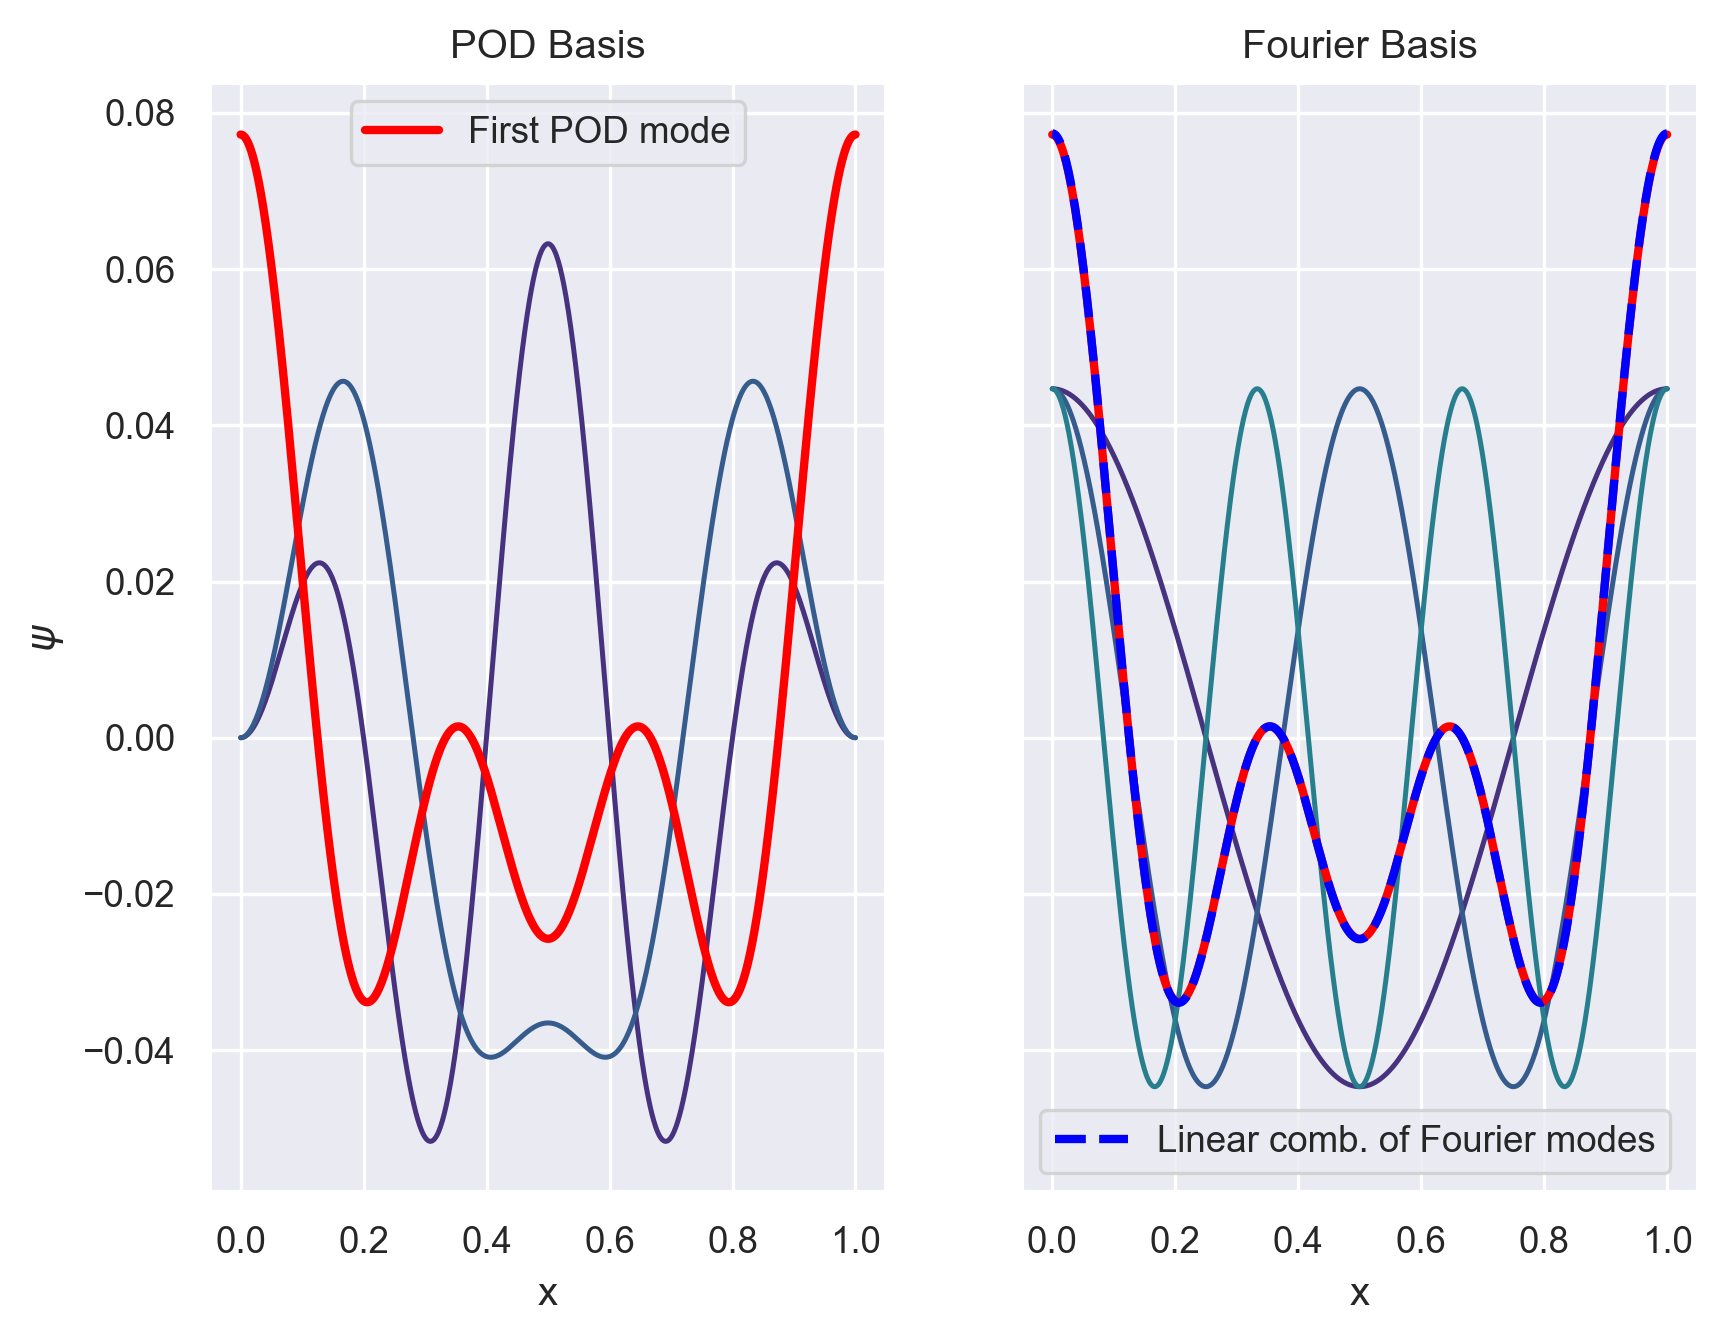
\includegraphics[width=\columnwidth]{research_project/piston/figures/svd_fourier/fourier_pod_bases.png}
    \caption{Fourier basis and its SVD transformation. 
    Since the Fourier basis is orthogonal, 
    the resulting SVD transformation is a linear combination of Fourier modes.}
\end{figure}

\subsubsection{(II) N-MDEIM with Fourier Basis}
To confirm our working hypothesis, 
we build the trilinear form 
(Equation~(\ref{eq:appendix_exact_representation_triliear_form}))
using the first five modes of the Fourier basis,
\begin{equation}
    \psi_q(x) = \qty{\cos(2 \pi \omega_q x) \, : \, \omega_q \in \qty{1, \ldots, 5}}.
\end{equation}
Since the Jacobian transformation is a linear function of time, 
despite the change in time of the domain, the trilinear form remains linear.
If there were no additional argument 
$\textcolor{blue}{\psi_k}$, 
we would only require one mode to represent the whole operator.
Therefore, we predict that we will only find 5 orthogonal resulting modes, that is, a non-hierarchical basis. 
This is confirmed by the singular value decay, 
shown in Table~\ref{tab:ndeim_with_fourier_modes}
(to be aligned with the code, a 0-indexing presentation is used).

\begin{table}[h]
    \centering
    \caption{Singular value spectrum for the N-MDEIM reduction with a Fourier basis.
    We have built the snapshots in time for two parameters and five Fourier modes.
    Since we know the resulting bases will be of the same size as the original input,
    we expect to have only 5 non-zero singular values, which is the case.
    To be aligned with the code, a 0-indexing presentation is used.}
    \begin{tabular}{cc}
        \toprule
        Singular index & $\sigma_i$ \\
        \midrule
        0 &  1.414 \\
        1 &  1.414 \\
        2 &  1.414 \\
        3 &  1.414 \\
        4 &  1.414 \\
        5 &  0.000 \\
        6 &  0.000 \\
        7 &  0.000 \\
        8 &  0.000 \\
        9 &  0.000 \\
        \bottomrule
    \end{tabular}
    \label{tab:ndeim_with_fourier_modes}
\end{table}
Again, as depicted by Figure~\ref{fig:appendix_fourier_nmdeim_reconstruction_error},
we obtain the same poor results in the approximation error when
we attempt to reconstruct the operator with a truncated basis. 

\begin{figure}[h]
    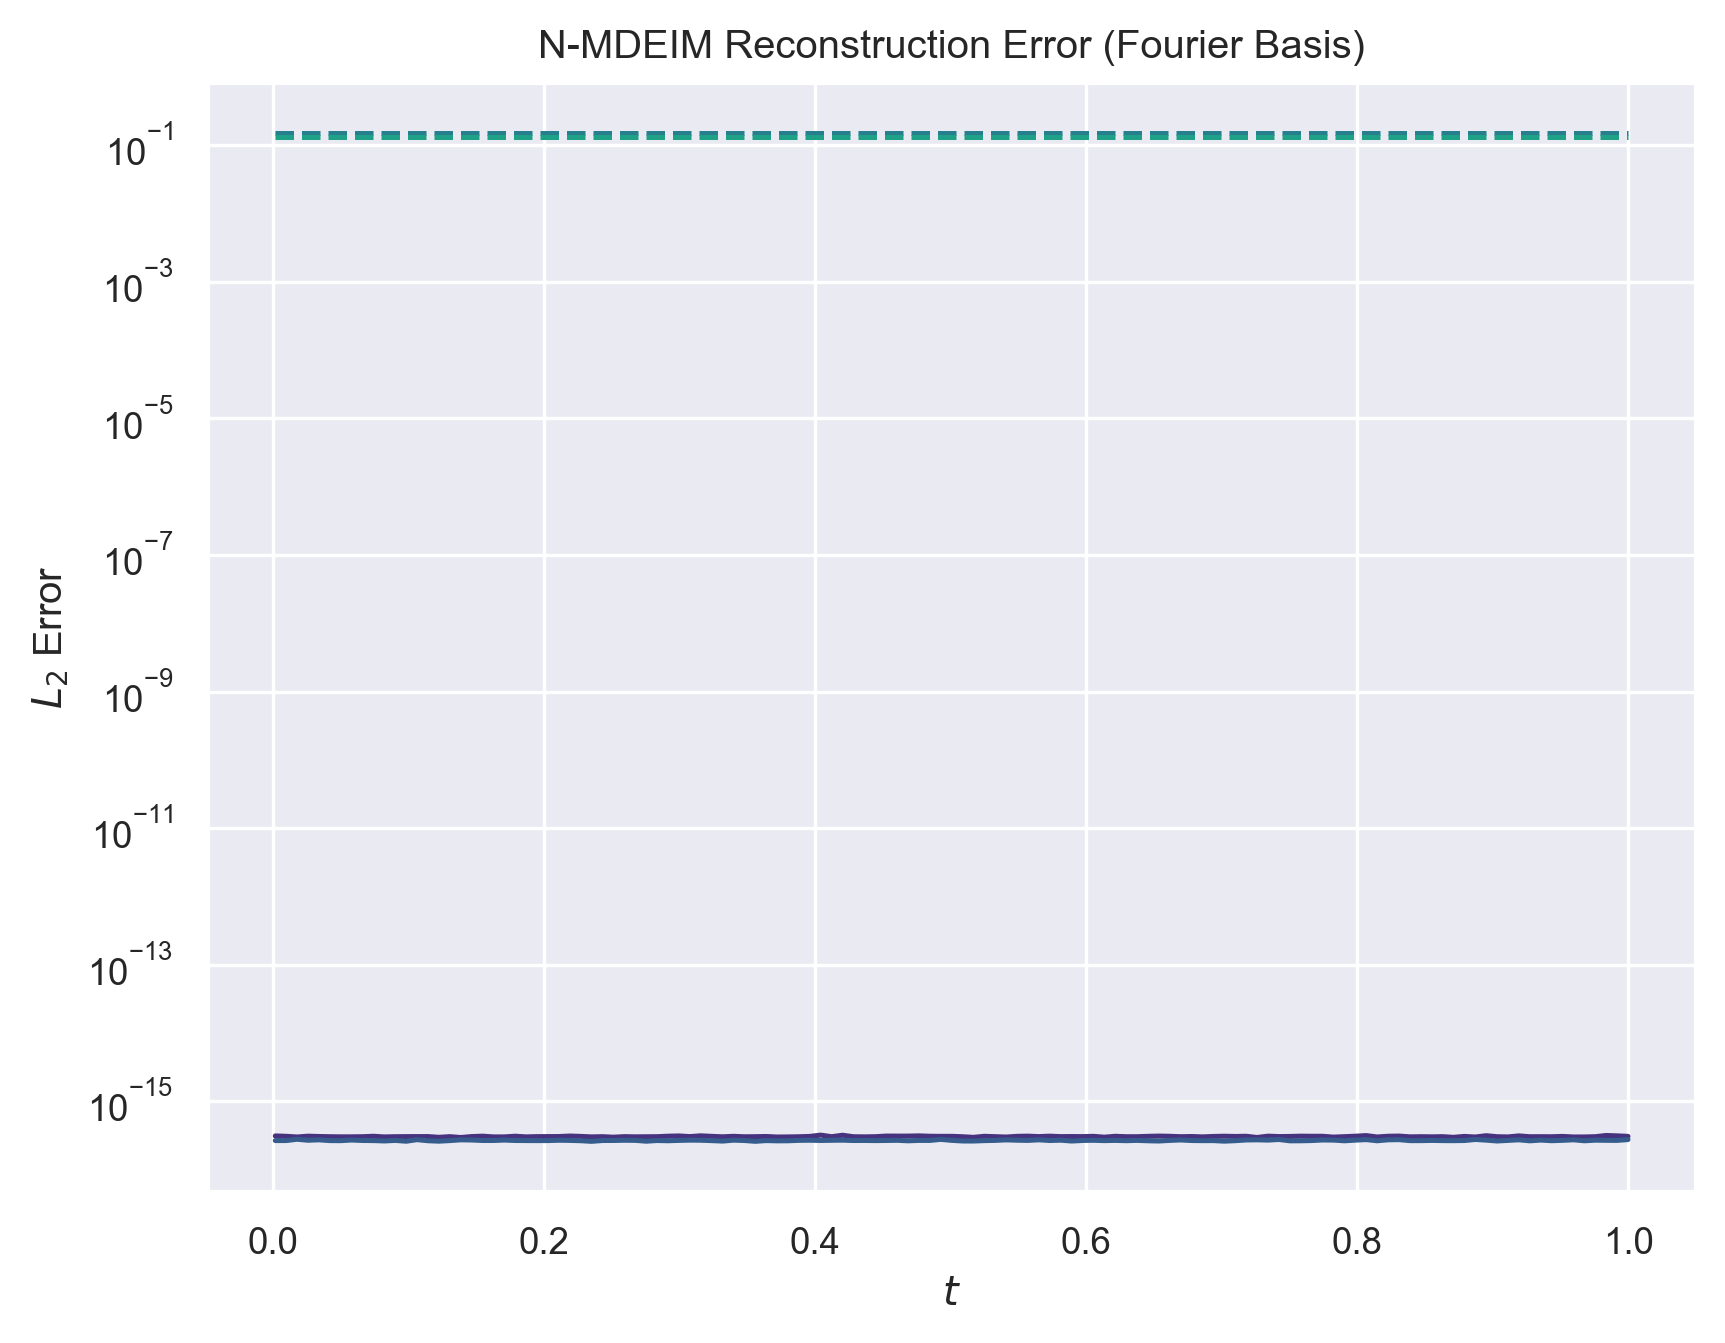
\includegraphics[width=\columnwidth]{research_project/piston/figures/svd_fourier/fourier_basis_mdeim_truncation_errors_comparison.png}
    \caption{N-MDEIM reconstruction error.
    The basis for this N-MDEIM has been built using 
    the first five Fourier modes to evaluate the trilinear form.
    According to the singular value decay, the basis is not hierarchical, 
    that is, all the operator modes (continuous) need to be used to 
    recover an accurate representation of the space.
    Hence, when one operator mode is removed (dashed), 
    the approximation error increases to unaffordable values for a simulation.}
    \label{fig:appendix_fourier_nmdeim_reconstruction_error}
\end{figure}
Now that we have been able to reproduce the same behaviour, 
and to validate our working hypothesis,
we go back to the use of RB solution modes.

% \newpage
\subsubsection{N-MDEIM with RB Solution Modes}
\label{sec:nmdeim_one_mode}
What would happen if we only used one mode from the RB solution modes to reduce the operator?
Could we use that basis to approximate the trilinear operator evaluated with other functions?
We take the first three RB solution modes 
and create a linear combination $f(x)$ with them,
\begin{equation}
    f(x) = 2 \psi_0(x) + \psi_1(x) + 3 \psi_2(x).
\end{equation} 
% This is shown in Figure~\ref{fig:appendix_rb_linear_combination}.
We now reduce the trilinear form with two strategies:
\begin{itemize}
    \item \mbox{(a) Subspace}: using only the first RB solution mode.
    \item \mbox{(b) Complete space}: using the three RB solution modes.
\end{itemize}

With each approach, we obtain a non-hierarchical orthogonal basis,
which we then use to reconstruct $\vb{N}_h\left(f(x)\right)$.
Since $f(x)$ is made out of the three orthogonal modes, 
we could expect approach (a) to fail.
However, it succeeds as well as approach (b).
This is proved by Figures~\ref{fig:appendix_rb_trilinear_num_1} 
and~\ref{fig:appendix_rb_trilinear_num_3}.
Additionally in Figure~\ref{fig:appendix_rb_trilinear_num_3} we have included 
the reconstruction error for the truncated base (we have removed operator mode). 

Using \textit{one} RB solution mode is sufficient to construct a perfect collateral basis
due to the linearity of the integrand within the trilinear form,
and the linearity of the Jacobian transformation.
Despite the fact that the function $f(x)$ contains other modes, 
the collateral basis built with one mode is able to reproduce its effect on the operator perfectly. 
% \begin{figure}[h]
%     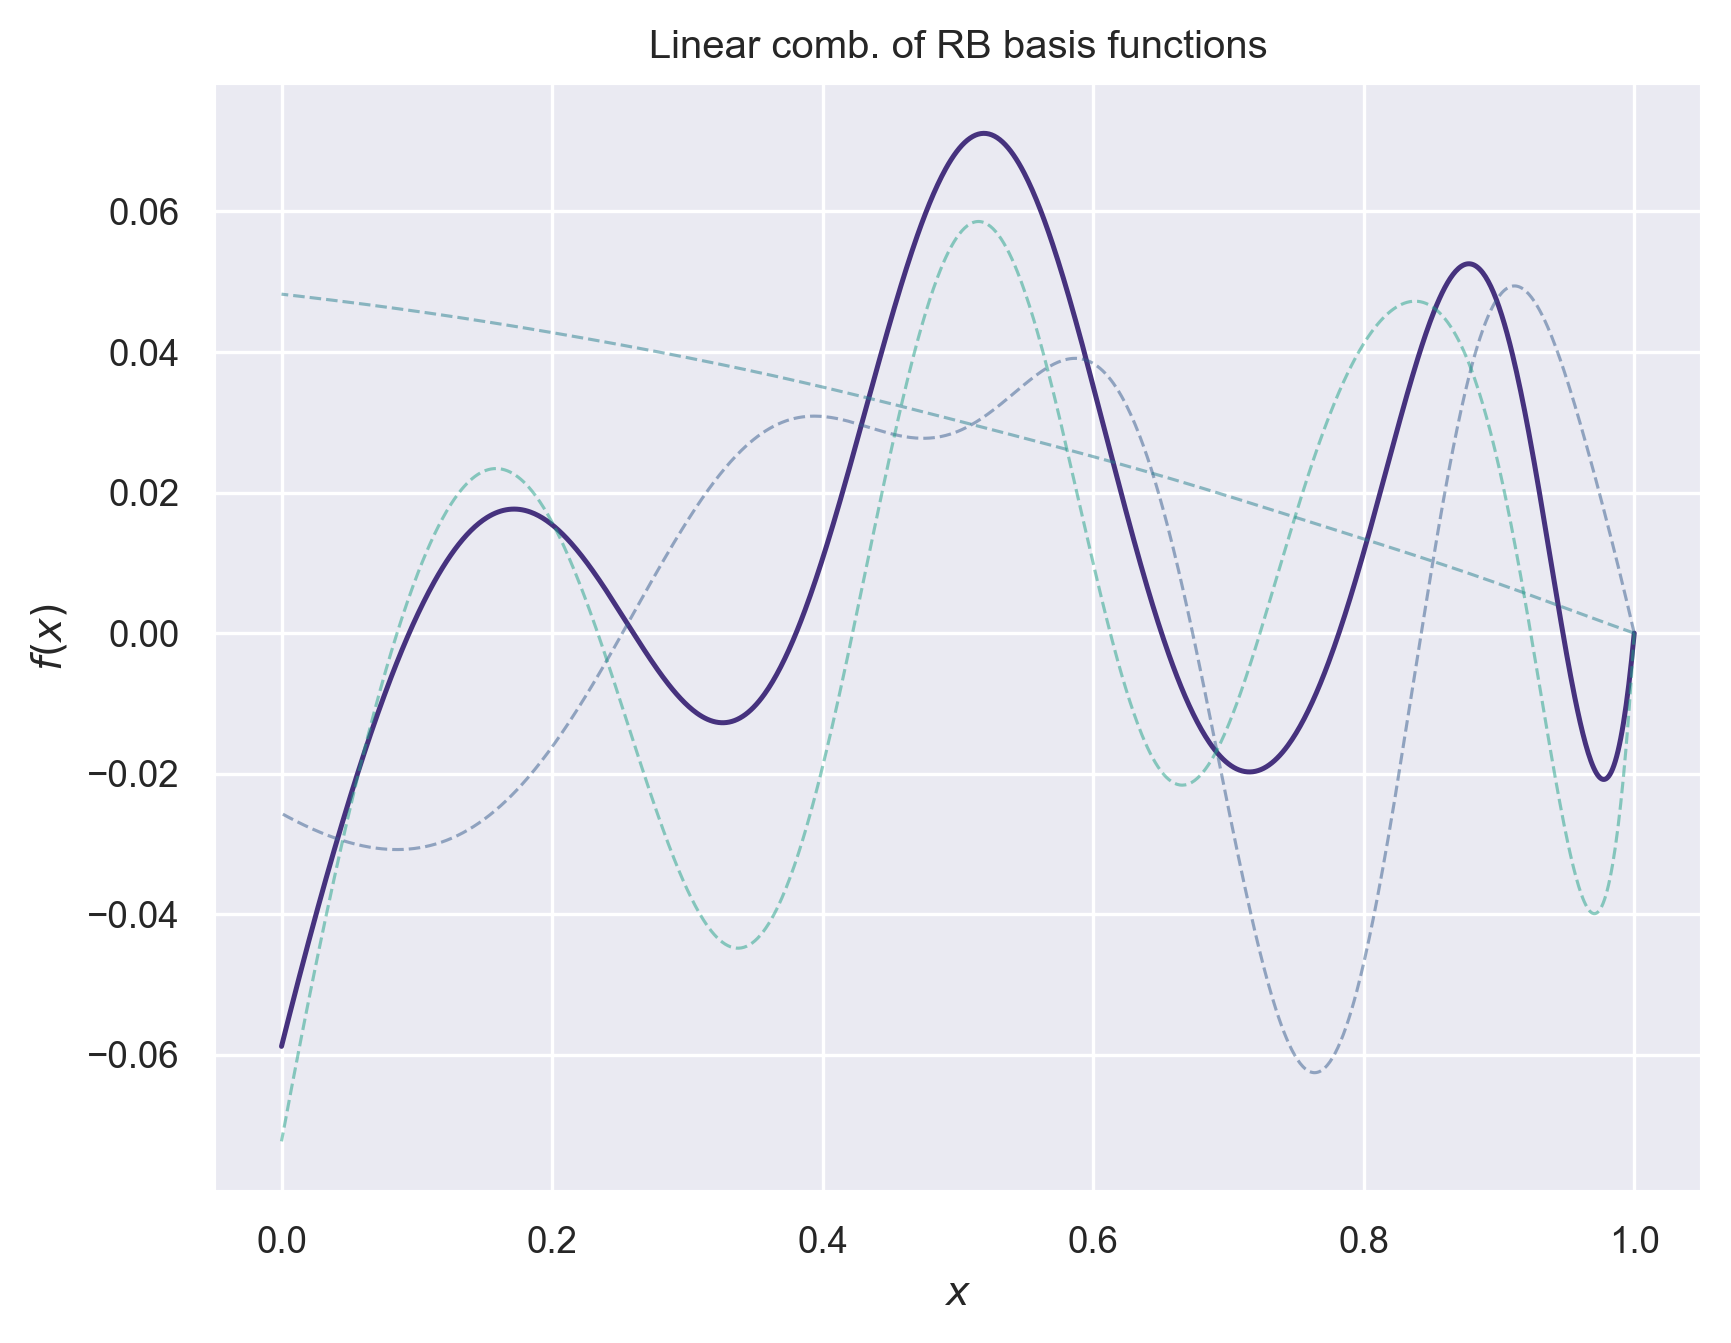
\includegraphics[width=\columnwidth]{research_project/piston/figures/svd_fourier/linear_combination.png}
%     \caption{First three RB solution modes and a linear combination $f(x)$ of them.  
%     The RB solution modes are shown in dashed.}
%     \label{fig:appendix_rb_linear_combination}
% \end{figure}
\begin{figure}[h]
    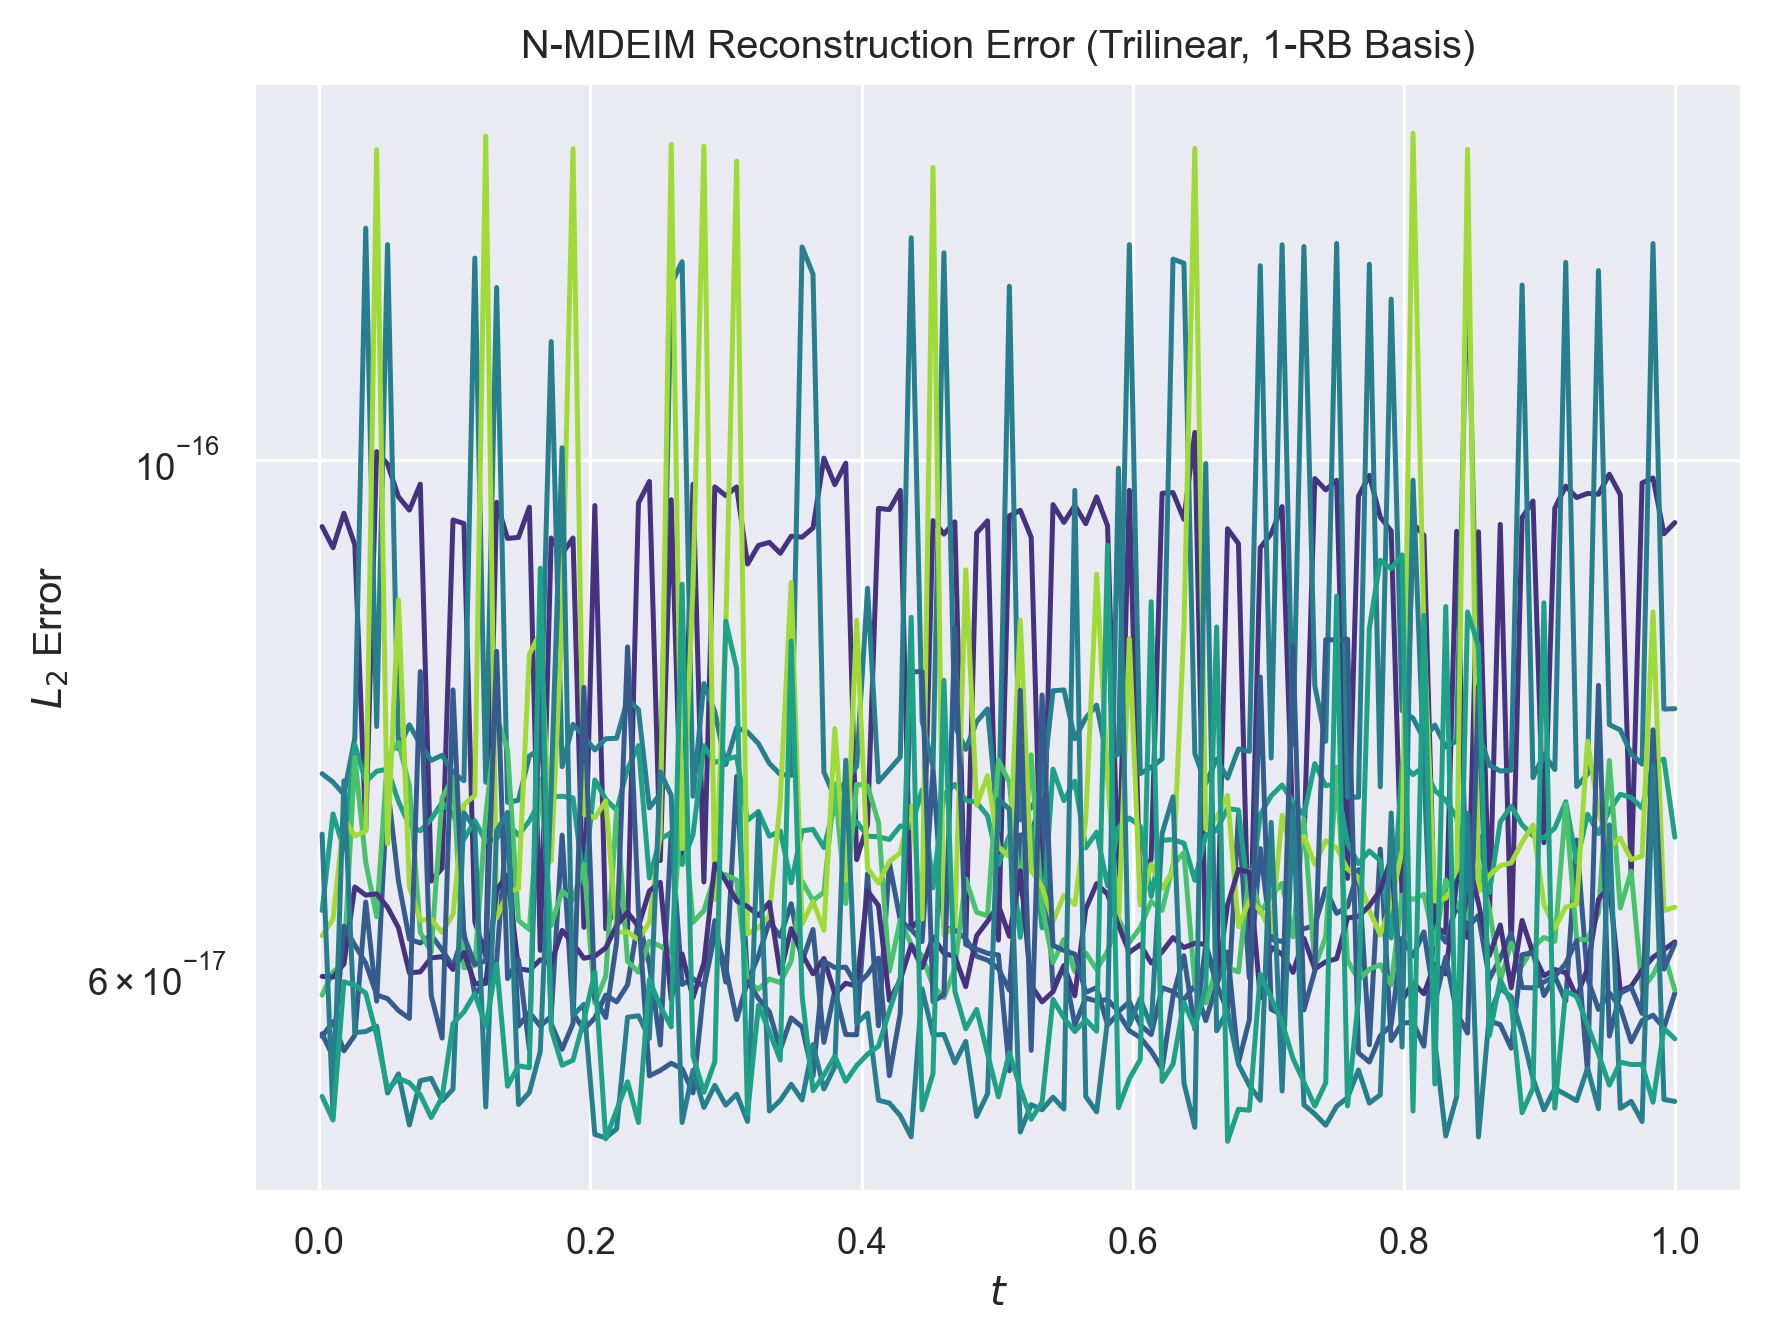
\includegraphics[width=\columnwidth]{research_project/piston/figures/svd_fourier/trilinear_nonlinear/rb_basis_mdeim_errors_trilinear_num_1.png}
    \caption{Reconstruction error for the trilinear operator evaluated with linear combination $f(x)$.
    The basis has been obtained only using the first RB solution mode.}
    \label{fig:appendix_rb_trilinear_num_1}
\end{figure}
\begin{figure}[h]
    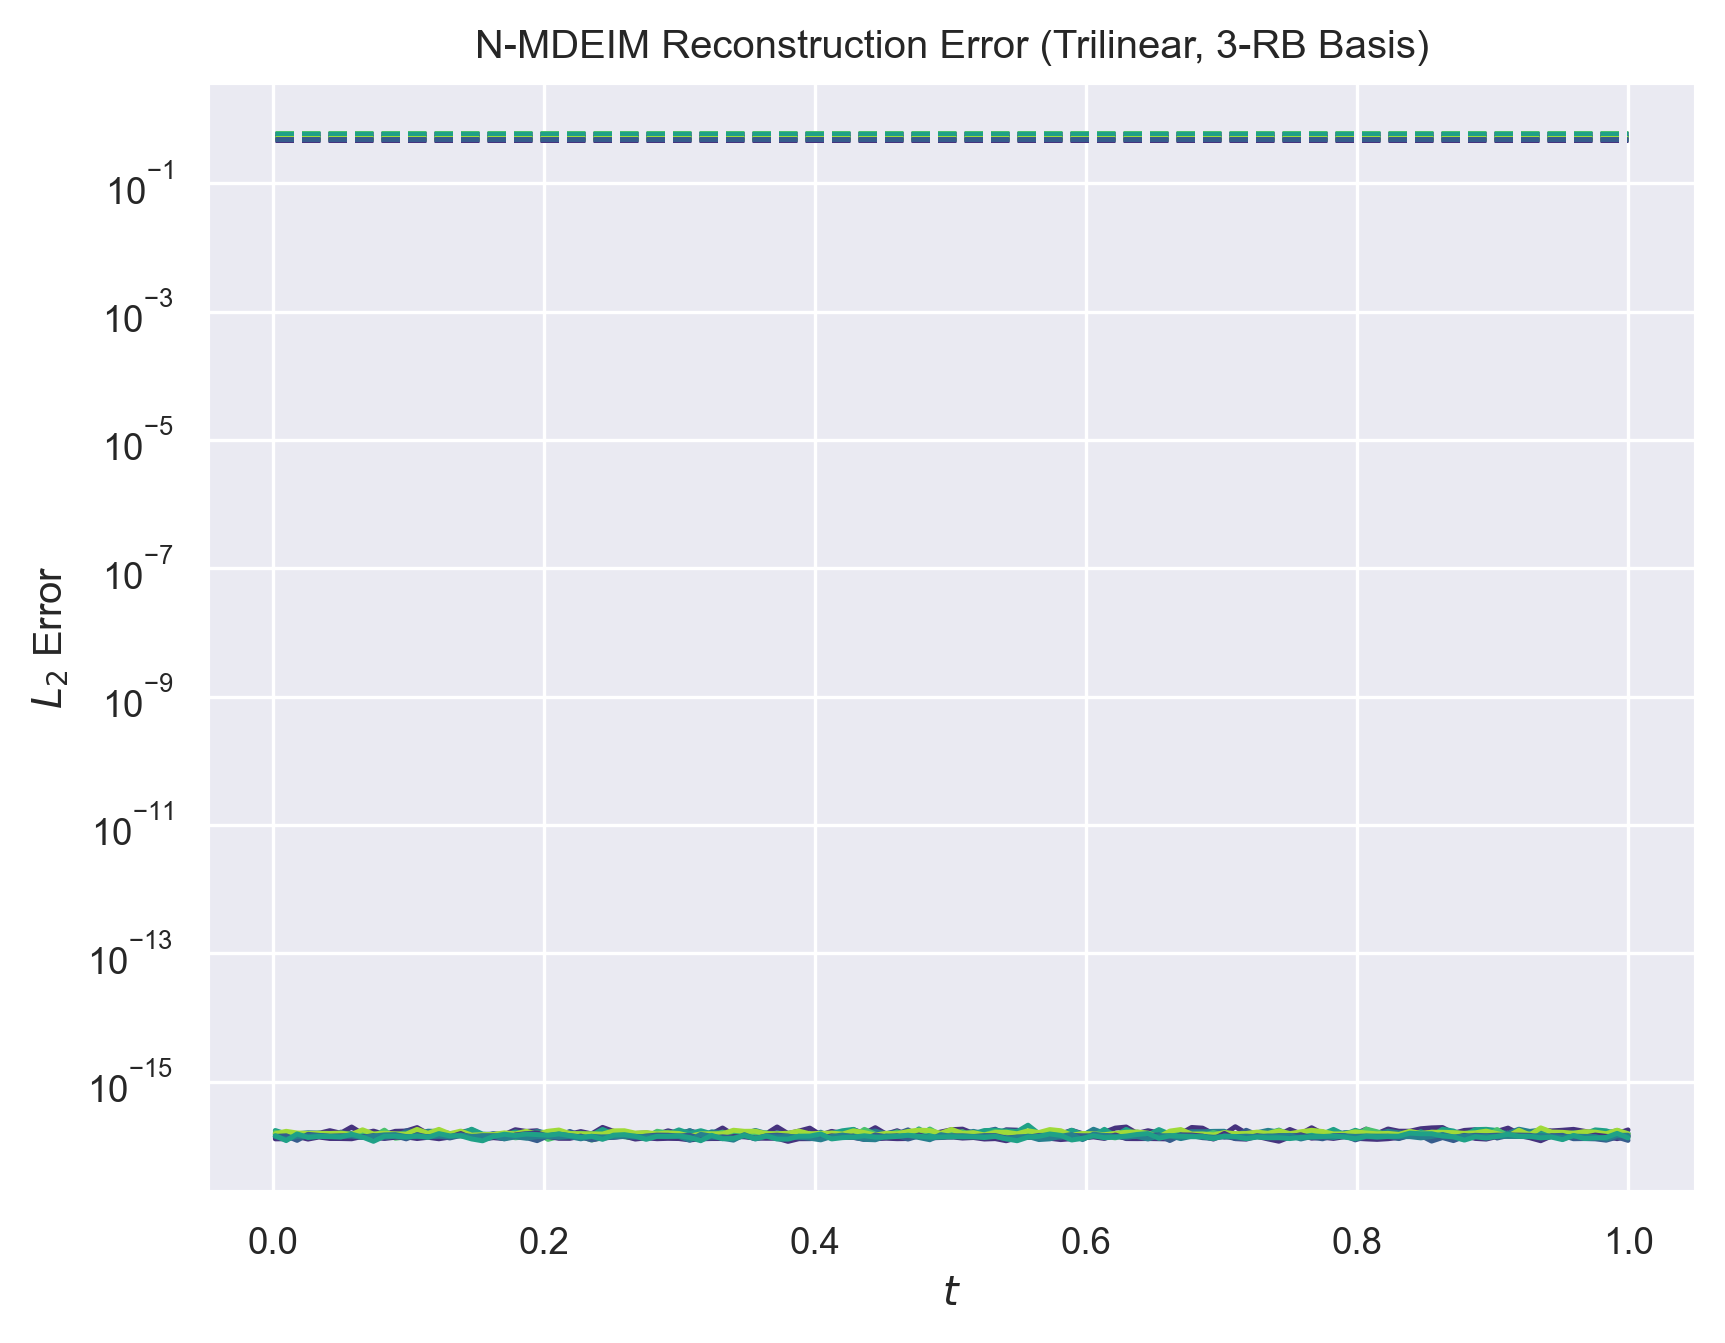
\includegraphics[width=\columnwidth]{research_project/piston/figures/svd_fourier/trilinear_nonlinear/rb_basis_mdeim_errors_trilinear_num_3.png}
    \caption{Reconstruction error for the trilinear operator evaluated with linear combination $f(x)$.
    The basis has been obtained using the three RB solution modes.
    In dashed is the approximation error using a truncated basis ($N=2$ operator modes). 
    The truncated basis shows a poor approximation error because the original basis is non-hierarchical, 
    hence all the operator modes are required to reconstruct the operator.}
    \label{fig:appendix_rb_trilinear_num_3}
\end{figure}
In the next section we explore what happens if a nonlinear function is present in the integrand.

\newpage
\subsubsection{N-MDEIM with a Nonlinearity in Space}
We have shown in the previous section how 
one can achieve a perfect collateral basis for the trilinear using exclusively one RB solution mode.

We now show results for a form with a nonlinear function inside the weak form, e.g., 
a non-uniform mesh displacement. 
Hence, we take on the reduction of
\begin{equation}
    \begin{split}
        \qty[\Ah{W}\left(\psi_{h}\right)]_{i,j}
        &= b_0 \inner{\psi_h(x) \cos(1+x) \grad \varphi_j}{\varphi_i}^{n+1},
        \\[2mm]
        &= b_0 \int_{0}^{L(t^{n+1})} \psi_h(x) \cos(1+x) \grad \varphi_j \varphi_i \dd x.
    \end{split}
\end{equation}
The results are shown in Figures~\ref{fig:appendix_rb_nonlinear_num_1} 
and~\ref{fig:appendix_rb_nonlinear_num_3}.
Both figures include the reconstruction error for a truncated base.

We find out that in the presence of a nonlinearity, 
it is unsufficient to use only one RB solution mode. 
When the basis built with approach (a) is truncated, the approximation error goes up 
to values near unity,
leading to poor reconstruction results.

Instead, when the first three RB solution modes are used to build the collateral basis,
truncating the outcome leads to a feasible basis.
The truncation leads to a higher approximation error, but still sufficiently small to produce
meaningful results if it were used in a simulation.    

\begin{figure}[h]
    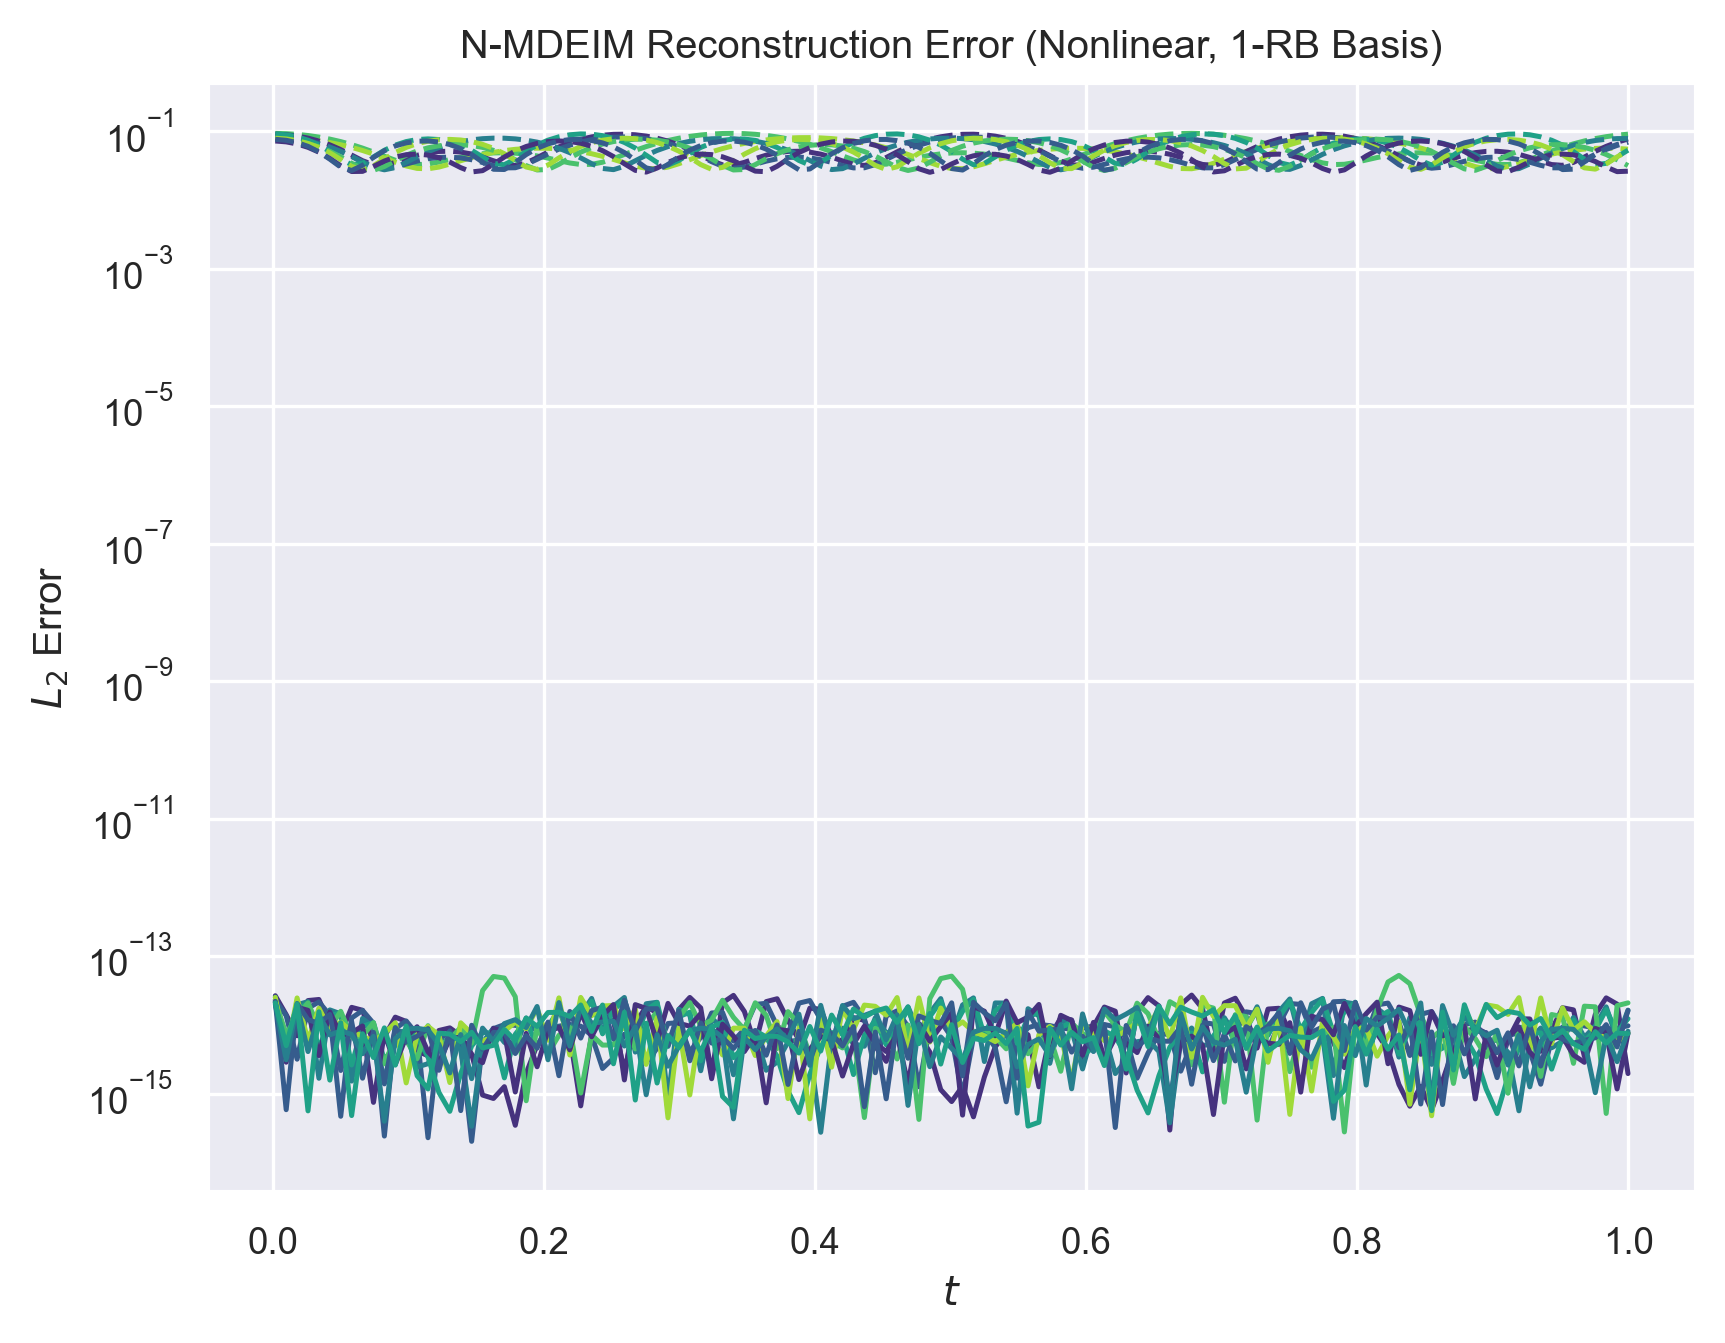
\includegraphics[width=\columnwidth]{research_project/piston/figures/svd_fourier/trilinear_nonlinear/rb_basis_mdeim_errors_nonlinear_num_1.png}
    \caption{Reconstruction error for the nonlinear operator evaluated with function $f(x)$.
    The basis has been obtained only using the first RB solution mode ($N_{\text{full}}=7$).
    In dashed is the approximation error using a truncated basis, 
    from which only one operator mode has been removed ($N_{\text{truncated}}=6$). 
    The truncated basis fails, due to the presence of the nonlinearity, 
    it is now unsufficient to use only one RB solution mode 
    to construct a collateral basis which accurately represents the whole space.}
    \label{fig:appendix_rb_nonlinear_num_1}
\end{figure}
\begin{figure}[h]
    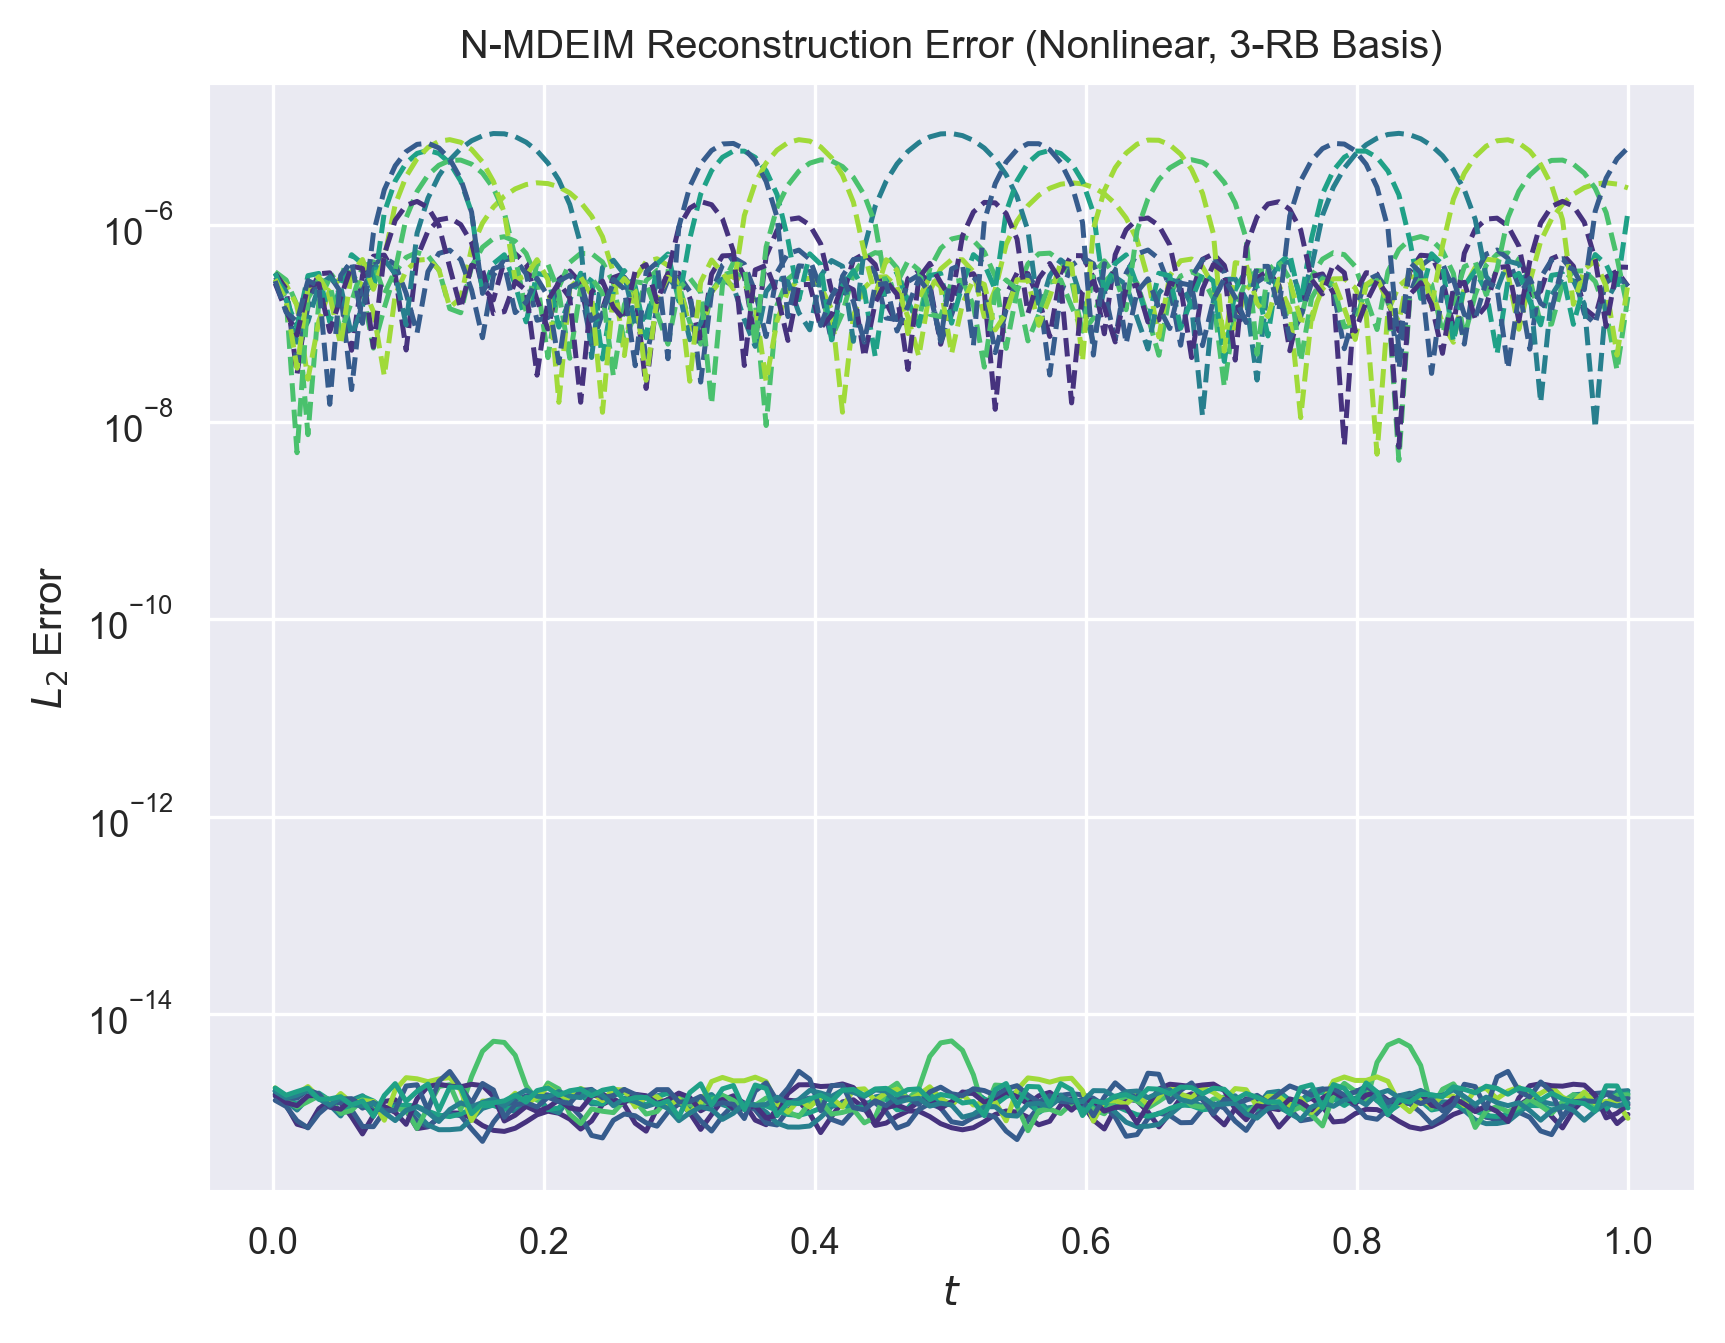
\includegraphics[width=\columnwidth]{research_project/piston/figures/svd_fourier/trilinear_nonlinear/rb_basis_mdeim_errors_nonlinear_num_3.png}
    \caption{Reconstruction error for the nonlinear operator evaluated with function $f(x)$.
    The basis has been obtained using the three RB solution modes ($N_{\text{full}}=19$).
    In dashed is the approximation error using a truncated basis, 
    from which several operator modes have been removed ($N_{\text{truncated}}=10$). 
    The truncated basis does not fail as drastically as the previous ones did, it simply presents a higher error,
    but still within an acceptable order of magnitude.}
    \label{fig:appendix_rb_nonlinear_num_3}
\end{figure}

\newpage
\subsubsection{Wrap-Up}
We have clarified the behaviour of the POD in the presence of a trilinear form 
and a linear Jacobian transformation.

Our first conclusion was that the POD of an orthogonal basis will produce
another orthogonal basis, as a linear combination of the input vectors.
This orthogonality is preserved under the linear transformation of the trilinear form.
As a consequence, the construction of the collateral basis can be achieved 
collecting snapshots with the evaluation of the trilinear form with 
only one RB mode.
If more RB solution modes are used to build the snapshots, 
the POD will return a larger collateral basis,
but one that will not have the hierarchical property.
That is, truncating that basis will consistently lead to poor approximation results.
The full basis will have to be used.
This is so because the SVD has created a linear combination of the orthogonal input snapshots.

In the presence of a non-uniform mesh movement,
the reduction trick of using one RB solution mode is unsufficient.
More RB solution modes have to be used to obtain 
a collateral basis that appropriately spans the whole domain.
Then, the basis is hierarchical, 
and allows for error control through basis truncation.

If we collect snapshots of the operator evaluated with the PDE solutions,
we couple the reduction of the RB space and the operator space.
Hence, it is best to reduce trilinear forms with RB solution modes.
If the trilinear form does not contain any spatial or time nonlinearity, 
one RB solution mode will be enough.
Instead, if nonlinearities are present within the integrand, more RB solution modes will be necessary 
to build a satisfactory basis.
One way or the other, this approach will reduce the number of snapshots to collect and compress,
leading to a lighter offline stage.
% We recall that the nonlinearity can be present implicitly, 
% as would happen if we assemble the matrix entries in the physical space under nonlinear mesh displacements effects.

\newpage
\subsection{Certification by Truncation}
\label{sec:hrom_results_posteriori_error_estimation}
To compute the HROM error in the preceding sections
we required the assembly and solution of the FOM model.
This is an undesirable fact, since if to validate our ROM solution
we need to compute its FOM counterpart, 
we are better off computing the FOM model straightaway
(which will be more accurate by definition).
Hence, we need an efficient a posteriori error estimator.

\subsubsection{Sacrificial ROM}
We use the model truncation technique.
That is, we carry with us \textit{two} ROMs,
with different basis sizes.
The additional ROM is called \textit{sacrificial} ROM (SROM).
It will be used to compute the actual error for the smaller ROM,
without requiring the calculation of the FOM.
% \mytodo{SROM: Create descriptive flow chart.}
By doing so, we bound the SROM error.
We assume it is smaller than the one of base ROM, since it contains more modes,
but we cannot know how much smaller it is.
Hence, we would bound the SROM errors by using a smaller ROM, 
but would use the SROM to calculate and present results.

For this error estimation procedure, the question we seek to answer is:
how many more modes does the SROM need to carry to estimate accurately the base ROM error?
Again, the answer to this question is problem-dependent,
but our approach to find it could be used for any problem.

\subsubsection{Error Estimation}
We depart from the error with respect to the FOM, which we seek to bound.
Then, we proceed to add and susbtract the solution from the sacrificial ROM,
\begin{equation}
    \norm{u_h - \rbV_{N} u_N} = \norm{u_h \pm \rbV_{\hat{N}} u_{\hat{N}} - \rbV_{N} u_{N}},
\end{equation}
where $\hat{N} > N$. 
By the triangle inequality, we get
\begin{equation}
    \norm{u_h - \rbV_{N} u_N} \leq \norm{u_h - \rbV_{\hat{N}} u_{\hat{N}}} + \norm{\rbV_{\hat{N}} u_{\hat{N}} - \rbV_{N} u_{N}}.
\end{equation}
If we define the error function $e_N = \norm{u_h - \rbV_{N} u_N}$, 
we get an upper bound of the desired error in terms of the sacrificial ROM error and the error between ROMs,
\begin{equation}
    e_N \leq e_{\hat{N}} + \norm{\rbV_{\hat{N}} u_{\hat{N}} - \rbV_{N} u_{N}}.
\end{equation}
With sufficient RB solution modes, it should be safe to assert that the error made 
with additional modes should be smaller or equal to the one made without it,
\begin{equation}
    e_{\hat{N}} \leq e_{N}.
\end{equation}
Thus, we get the following error bound,
\begin{equation}
    e_N \leq \norm{\rbV_{\hat{N}} u_{\hat{N}} - \rbV_{N} u_{N}},
\end{equation}
It remains to determine how sharp this error estimate is.

\subsubsection{Error Between Two ROMs}
The error estimator 
\begin{equation}
    \tilde{e}_{N}(\hat{N}) = \norm{\rbV_{\hat{N}} u_{\hat{N}} - \rbV_{N} u_{N}}
\end{equation}
can be expressed as a sum in terms of the RB solution modes.
Due to the hierarchical character of the RB basis, 
$\rbV_{\hat{N}}$ contains the same columns 
up to $N$ as $\rbV_{N}$.
Thus, the error between ROMs can be expressed as
\begin{equation}
    \begin{split}
        \norm{\rbV_{\hat{N}} u_{\hat{N}} - \rbV_{N} u_{N}} 
        = \\ 
        \norm{
        \sum_{i=N+1}^{\hat{N}} u^{\hat{N}}_{i} \psi_{i} 
        + 
        \sum_{j}^{N} (u^{\hat{N}}_{j} - u^{N}_{j}) \psi_j
        }.
    \end{split}
\end{equation}
The difference $(u^{\hat{N}}_{j} - u^{N}_{j})$ between ROM coefficients is relatively small, 
since it represents the difference between the two coefficients associated to the same mode.
If they were notably different, 
it would mean that the dynamics between the original ROM and the sacrificial one are different.
Since the RB solution basis is hierarchical, 
this will not be the case for sufficiently well resolved ROMs: 
adding an additional mode should only refine the solution, 
not change drastically how the previous modes are scaled.
They are not strictly the same because the ROM matrix changes if more modes are added to the basis,
but again, it does so in a way that dynamics are preserved.

In Figure~\ref{fig:estimator_accuracy_timewise} we show in the behaviour of the error estimator 
for each time step.
In Figure~\ref{fig:estimator_accuracy} 
we present how close the estimator is to the actual error,
where both are aggregated in the time direction.
We have computed the estimator for~\mbox{$\Delta N = 1, 5$} and~$10$ additional modes.
Then, we compute \textit{estimator accuracy}, how far it is from the actual ROM error,
aggregated for all time steps, 
% \mytodo{Esitmator accuracy: make this a relative error.}
\begin{equation}
    \text{Estimator Accuracy} = \norm{e_t - \tilde{e}_t} 
\end{equation}
We conclude that it seems to be better to carry more than one mode.
Nevertheless, if to compute all these additional modes becomes too costly,
one extra mode will produce a valid estimator, provided that the base ROM is well resolved.
Later on in Section~\ref{sec:certification_limits} we explore the limits of this certification technique.

\newpage
\begin{figure}[h]
    \centering
    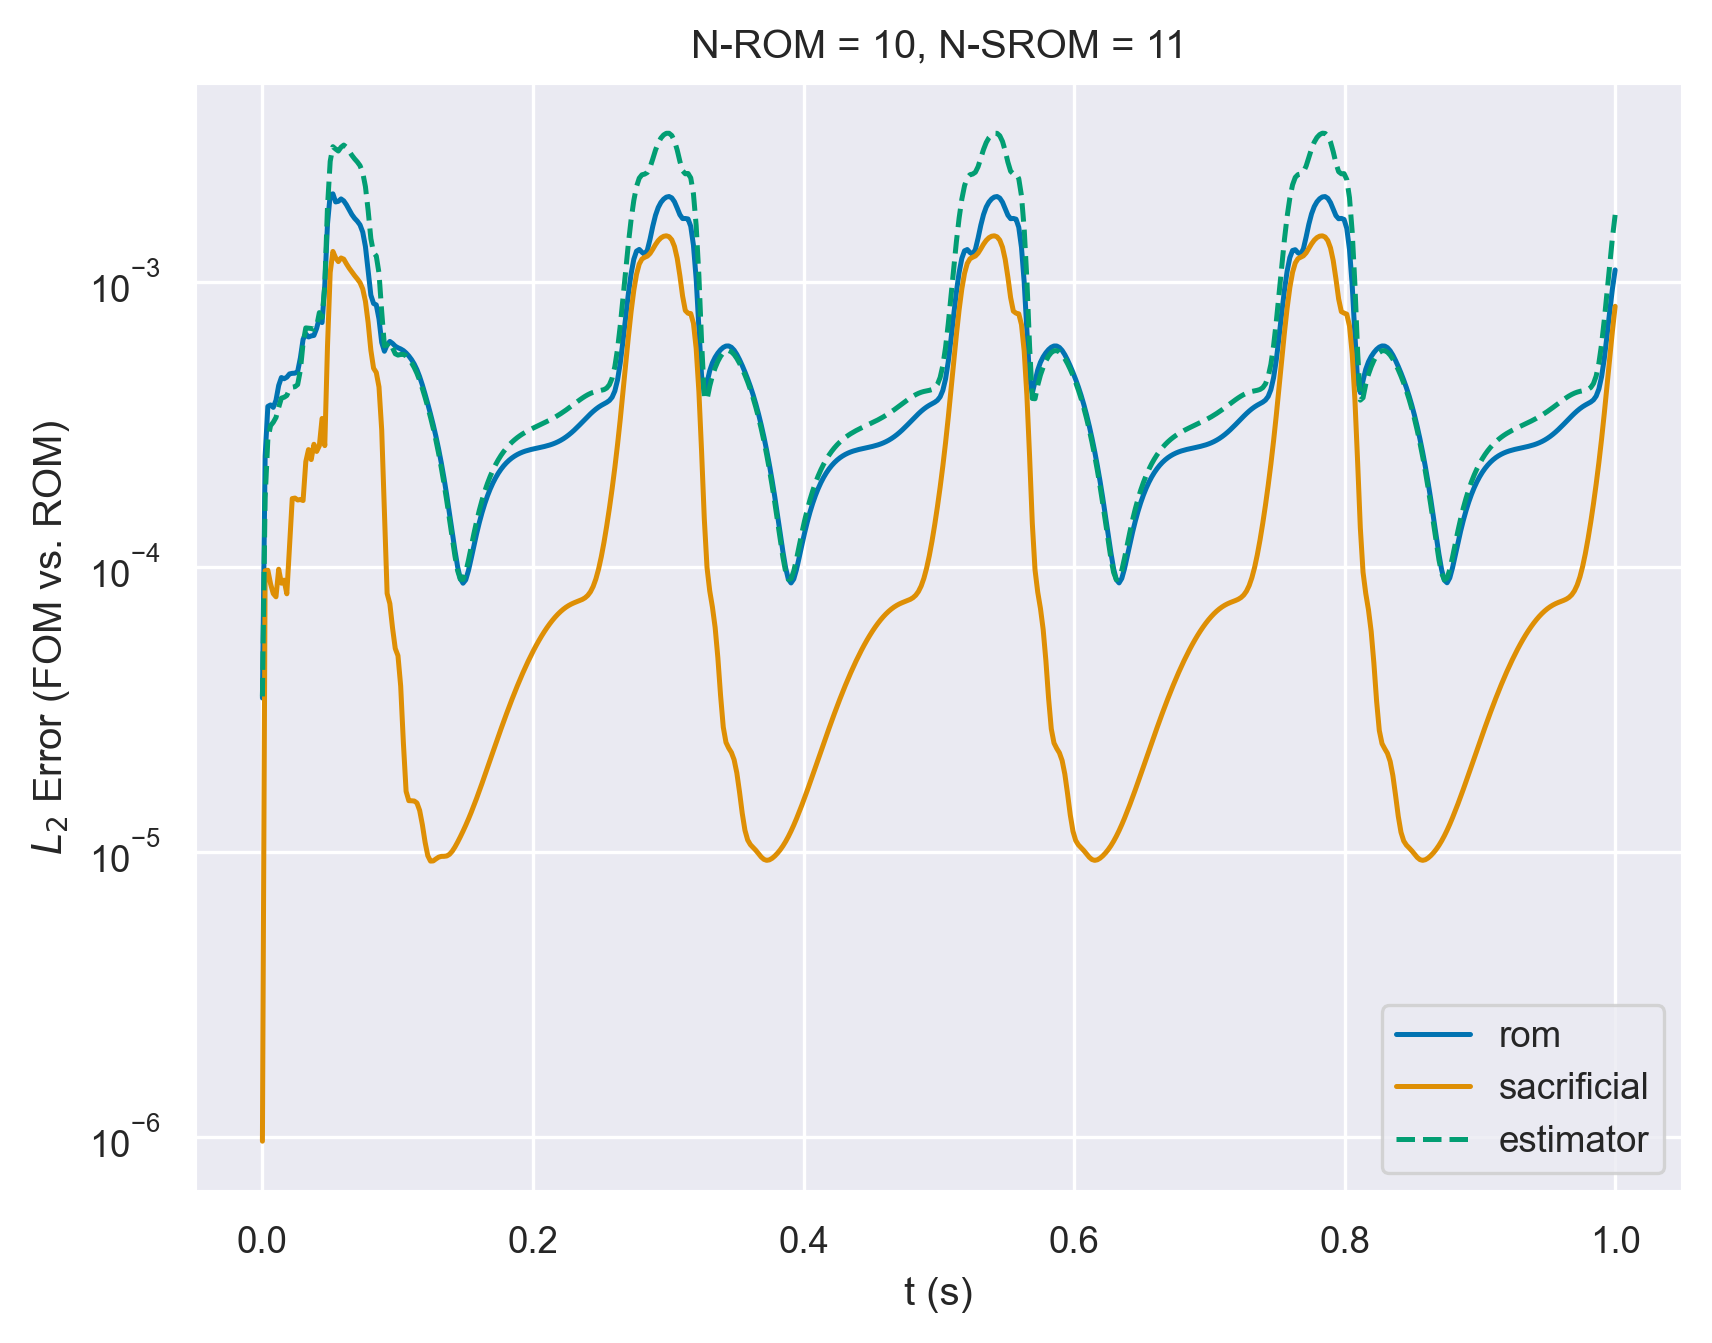
\includegraphics[width=1\columnwidth]{research_project/piston/figures/rb_certification/error_estimation_rom_10_srom_11.png}
    \caption{Time-wise a posteriori error estimator accuracy for $N_{\text{ROM}} = 10$, $N_{\text{SROM}} = 11$.
    We observe how accurate the estimator is carrying only one additional mode.}
    \label{fig:estimator_accuracy_timewise}
\end{figure}
\begin{figure}[h]
    \centering
    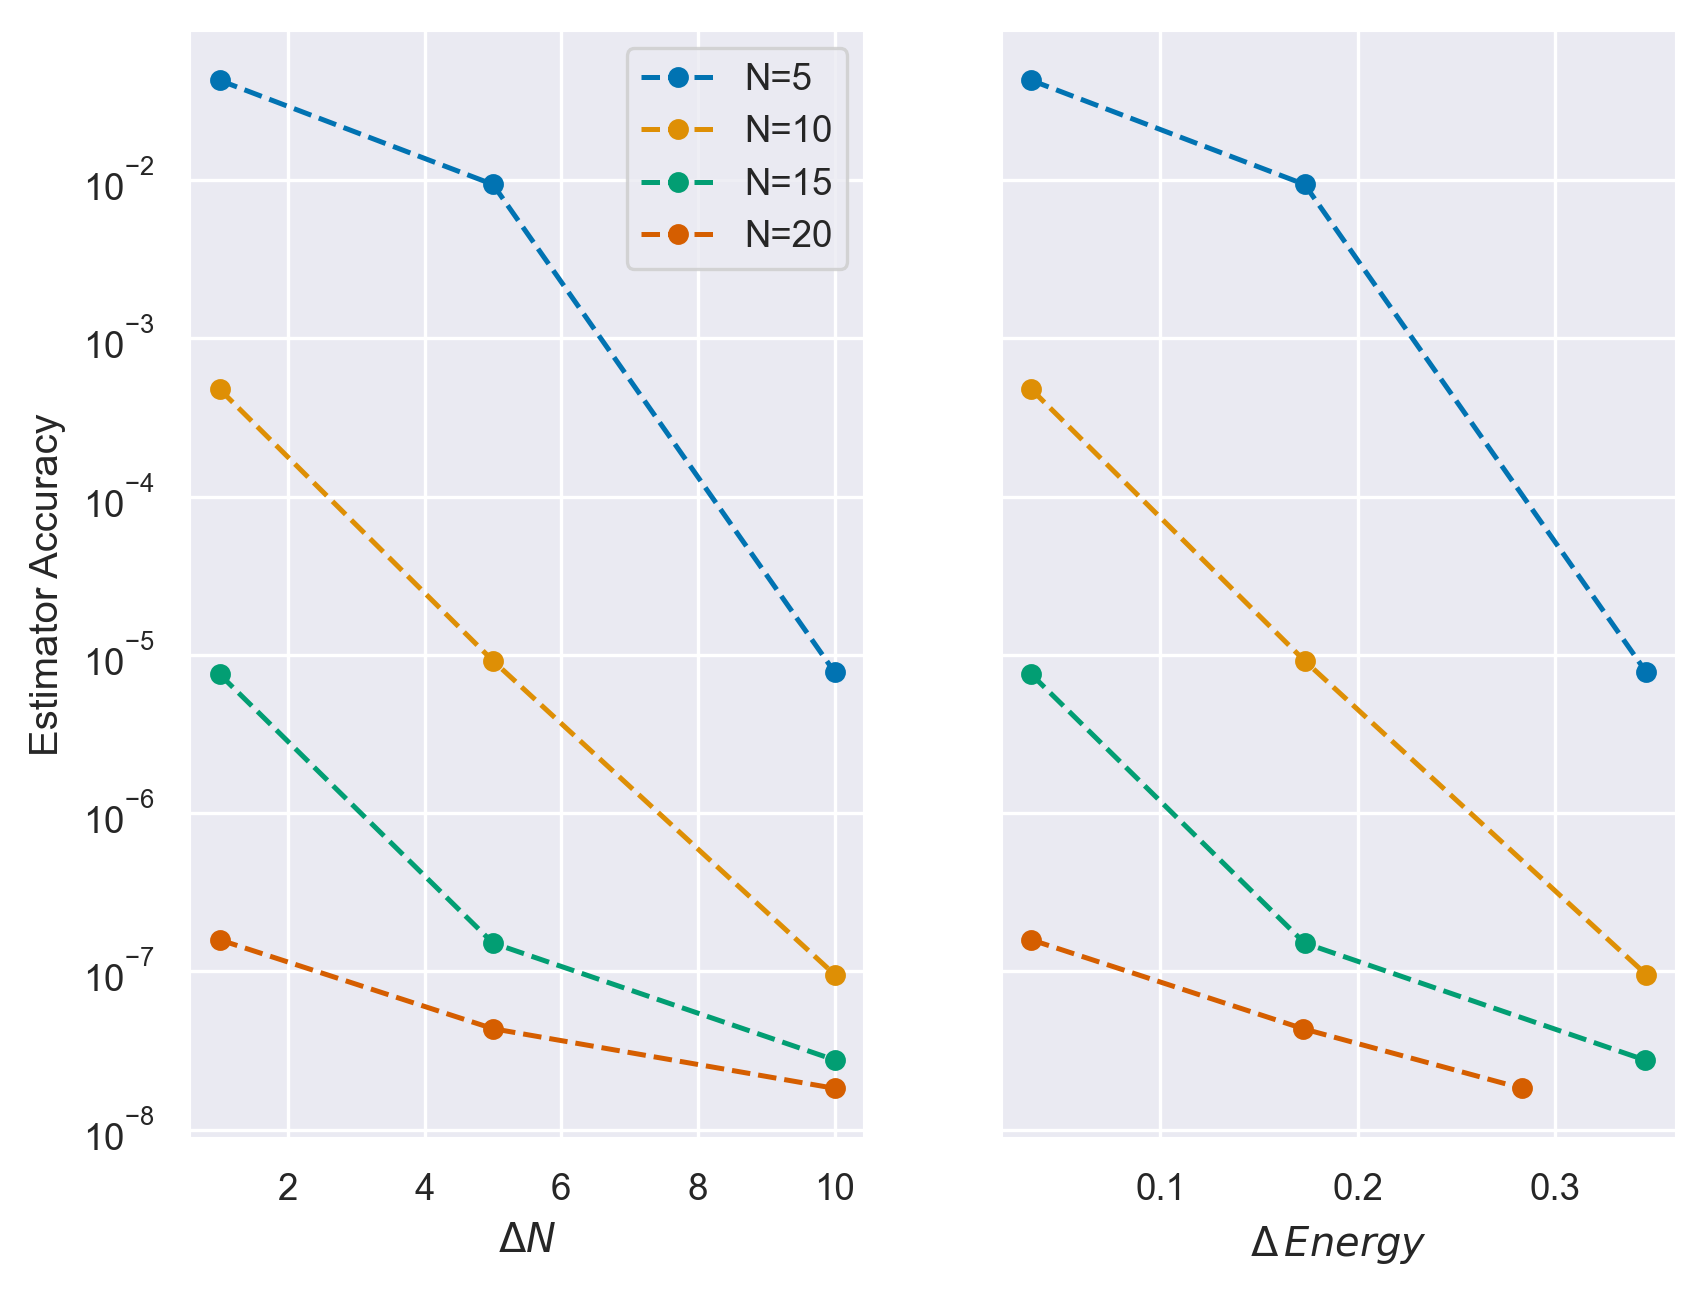
\includegraphics[width=1\columnwidth]{research_project/piston/figures/rb_certification/estimator_accuracy.png}
    \caption{A posteriori error estimator accuracy.
    We see how it can become more effective to carry more additional modes than rather just one.}
    \label{fig:estimator_accuracy}
\end{figure}

\clearpage
\subsection{Results for Non-Uniform Mesh Stretching}
\label{sec:arbitrary_mesh_results}
We now present results for a non-uniform mesh displacement. 
% We present the reduction achieved by the nested POD.
% We recall that this algorithm is used for the solution and the snapshots of each operator.
% The reduction methodology introduced by the (M)DEIM technique 
% is the selection of the interpolation entries, 
% which will guarantee a correct approximation of the operator when they are exactly matched.
In Table~\ref{tab:nlinear_disp_bases_size} we give the resulting basis size 
for each operator at each step of the nested POD.
The final size (\mbox{"Param. space"} column) is sufficient to accurately reconstruct the operators.
% As opposed to the initial scenario of uniform cell distortion, 
% where the Jacobian was only a function of time, we
All operators require more than a trivial number of elements, 
but the bases size differ.
% The most difficult operator is the trilinear one.
The trilinear term snapshots have been obtained from the FOM simulation 
($u^{*}$-general).
% Since these snapshots contain simultaneously 
% the effects of the solution 
% and the nonlinear Jacobian,
Again, the reduction of this operator requires as many terms as the solution space.

We have purposefully used a different parameter sampling size 
for the FOM simulation and the collection of operator snapshots;
to show a weakness of this methodology.
Assembling operators is a time-consuming operation, 
but it is cheaper than carrying out a full FOM simulation.
Hence, it is encouraged to have a methodology which splits the collection
of operator snapshots and solution snapshots.
The former are cheaper to obtain than the latter, 
and hence a larger parameter space can be sampled to produce a richer collateral basis.
By richer basis we intend one that is likely to work better during the online stage, 
for it has potentially a higher generalization degree.

A possible scenario where the split between the assembly and snapshot-collection steps
is not feasible is one where the displacement had to track the solution of the PDE,
e.g. in fluid-structure interaction.
In that case we have no alternative but to collect 
\textit{all} the snapshots (operators and solution) from FOM simulations.
% knowing that the reduction will deal with both effects simultaneously. 

% Within the operators which do not depend on the solution,
% the most difficult one is the \textit{Stiffness} operator. 
% We believe this is so because it contains two gradient operations,
% on the test and trial functions respectively.
% A gradient operation implies the existence of an inverse mesh size term \mbox{$h^{-1}(x,t)$}.
% Since the mesh is no longer uniform, 
% the interaction \mbox{$h_{i}^{-1} h_{j}^{-1}$} between the two gradients will produce a tougher nonlinearity
% than the one produced by a single gradient or none, 
% as shown by the reduction of the remaining operators.

\begin{table}[h]
    \centering
    \caption{Basis size at each step of the nested POD strategy.
    The operators are sorted by collateral basis final size.
    The Nonlinear-lifting operator corresponds to the cross-term lifting matrix
    that arises from the nonlinear convective term.}
    \begin{tabular}{lccc}
        \toprule
        {} &  Time int. ($N_t = 500$) &  Param. space & $N_{\mu}$ \\
        \midrule
        Reduced-basis     &                     660 &          93 & 20 \\
        \midrule[0.01mm]
        Trilinear         &                     670 &          94 & 20 \\
        Stiffness         &                     121 &          68 & \multirow{5}{*}{30} \\
        Rhs               &                     180 &          32 &  \\
        Mass              &                      60 &          21 &  \\
        Convection        &                      60 &          20 &  \\
        Nonlinear-lifting &                      60 &          19 &  \\
        \bottomrule
    \end{tabular}        
    \label{tab:nlinear_disp_bases_size}
\end{table}
In Figure~\ref{fig:nlinear_disp_sep_loglog} we show 
the singular value decay (SV decay) for each operator.
% Top plot
On the top plot, we present the decays for each time integration path 
(for a fixed parameter, they represent the branches of the treewalk).
These decays correspond to the first compression of the snapshots, 
with which we obtain a basis $\Psi_{\mu_i}$ for a specific parametrization.
% Bottom plot
On the bottom plot, we present the decay of the final POD step, 
which compresses (for each operator) all of the previous bases into one.

% Zoom-in
% We observe how the Stiffness and RHS operators are tougher to reduce in time,
% and hence also in the parameter space.
In Figure~\ref{fig:nlinear_disp_sep_logy} we present 
a zoom-in for the first ten singular values.
This shows how some operators are reduced 
to very few modes in the time direction.

% Discussion 
Indeed, in the time direction most operators still remain simple to reduce, 
but when each parameter-fixed basis is compressed with the others,
most information is retained.
This is so because the mesh parameters have a nonlinear effect, 
whereas time has a linear one.
That is why in time it is simple to reduce the operator,
but not so much across the geometrical parameter space.
When we were dealing with a uniform deformation of the mesh,
since the stretching parameter $\delta$ is present linearly,
the piston oscillation can be captured by sampling one parametrization,
two\footnote
{
    The oscillating frequency $\omega$ is inside a sinusoidal function,
    but this was only relevant for the mesh velocity, 
    not the overall displacement.
} at most.

\subsubsection{Operators Error Decay}
Now that we have multiple operators with a non-trivial basis, 
we have to tune all of their errors simultaneously.
We plot in Figure~\ref{fig:nlinear_disp_operators_error_decay}
the error decay for each operator as a function of the basis percentile size.
The offline and online sampling pools are shown in
Figure~\ref{fig:nlinear_disp_operators_sampling_space} in the Appendix.

All the errors decay as the basis size increases, 
but each operator needs a different basis size to reach the same error threshold.
For the offline samples, as the basis size is shrunk, 
the errors remain concentrated for different parametrizations.
For the online samples, this behaviour is not present, 
with more dispersion between the different parametrizations.
The errors with the full basis are smaller for the offline pool, 
compared to those from the online pool.
This is an expected behaviour, 
since the basis is optimized for the offline sample.

\begin{figure}[h]
    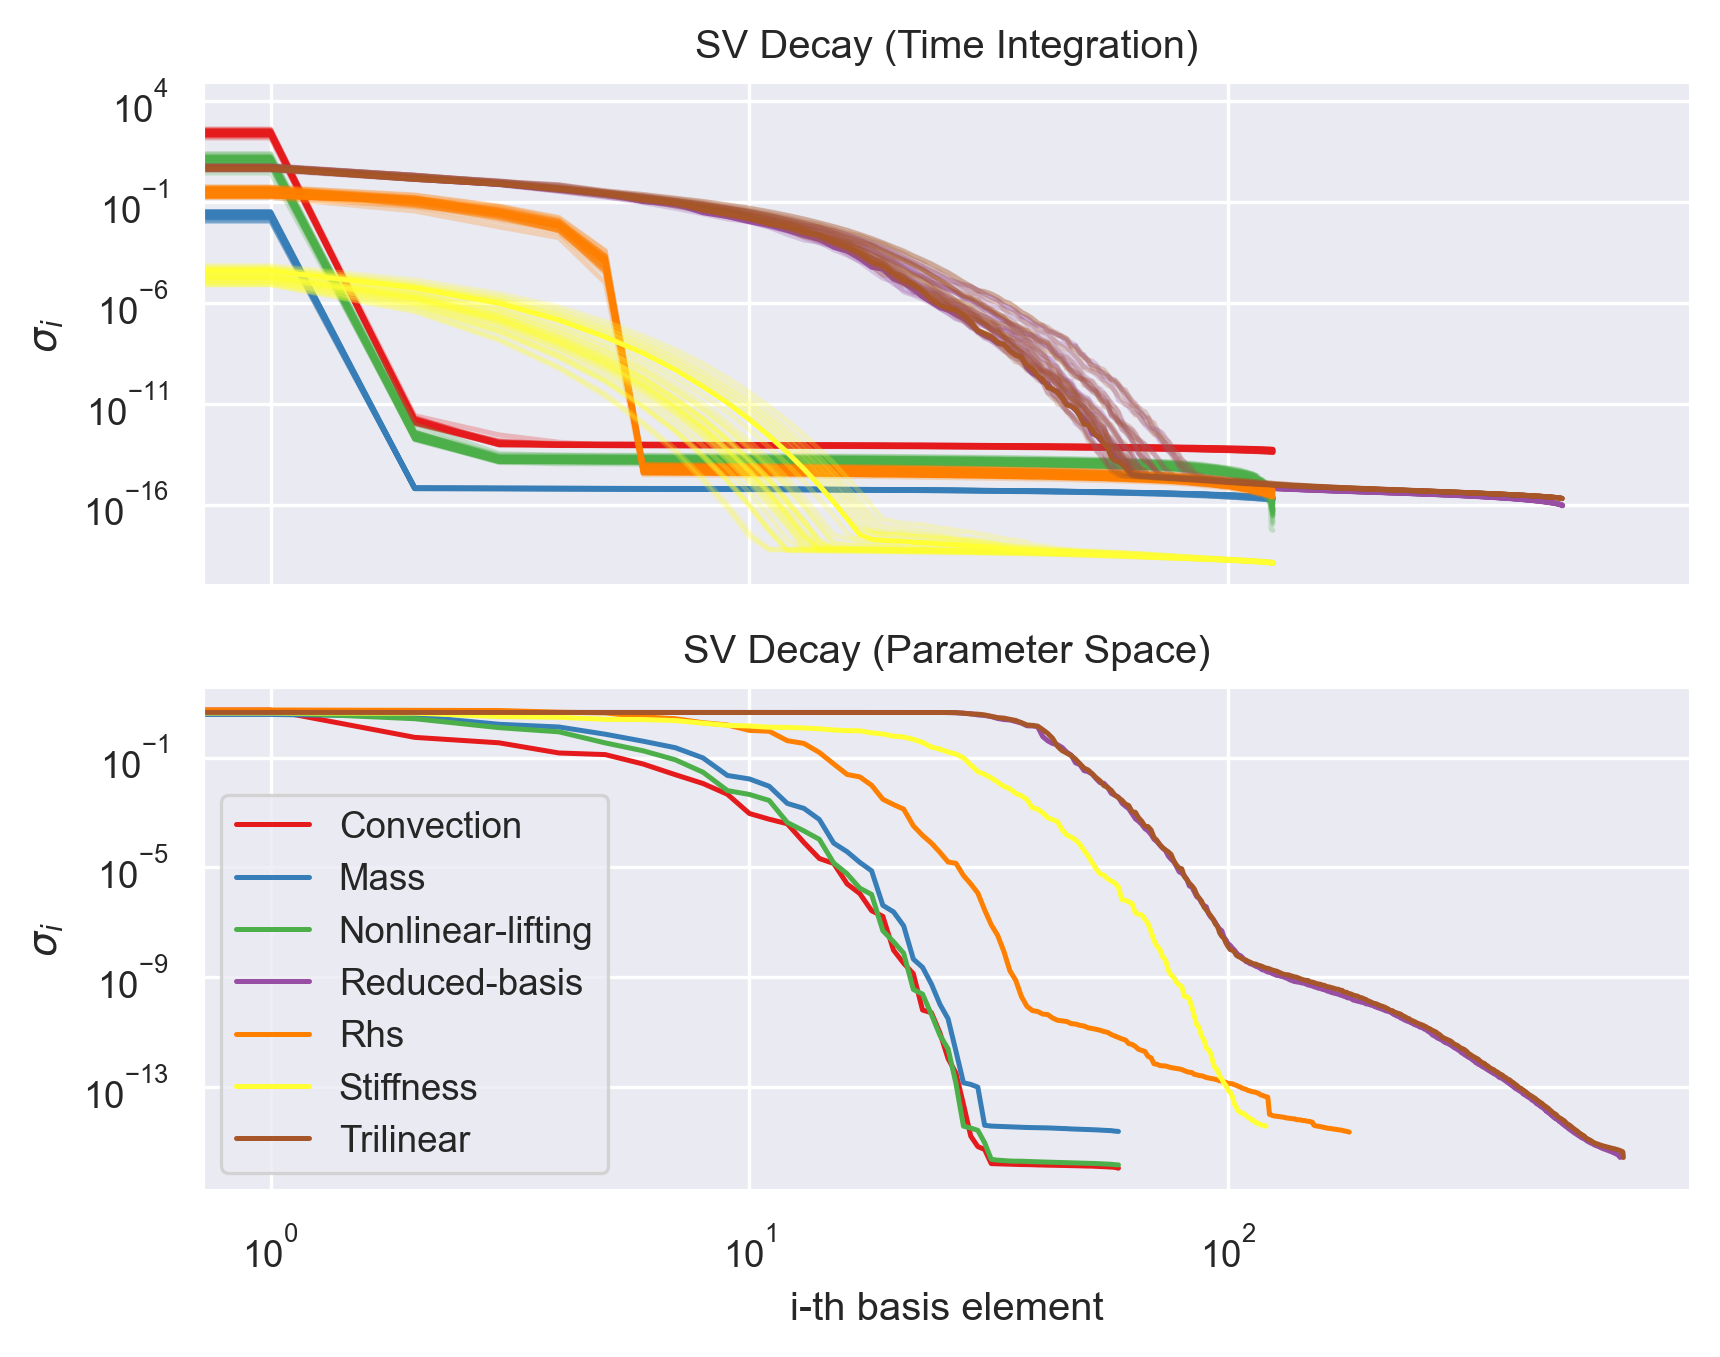
\includegraphics[width =\columnwidth]{research_project/piston/figures/nonlinear_displacement/separable/sigmas_loglog.png}
    \caption{Singular value decay for the two nested POD steps: 
    \mbox{time integration} (top) and \mbox{parameter space} (bottom).
    Both axes are represented in logarithmic scale.
    We observe how due to the presence of the non-uniform displacement
    the operators are no longer trivially reduced.
    It takes several basis terms to accurately represent 
    the effects of the nonlinearity.
    The solution space and the trilinear operator have an identical decay.
    This is so because the trilinear form is equally affected by the 
    values of the extrapolated velocity $u^{*}$ 
    and the effects of the non-uniform displacement.}
    \label{fig:nlinear_disp_sep_loglog}
\end{figure}

\begin{figure}[h]
    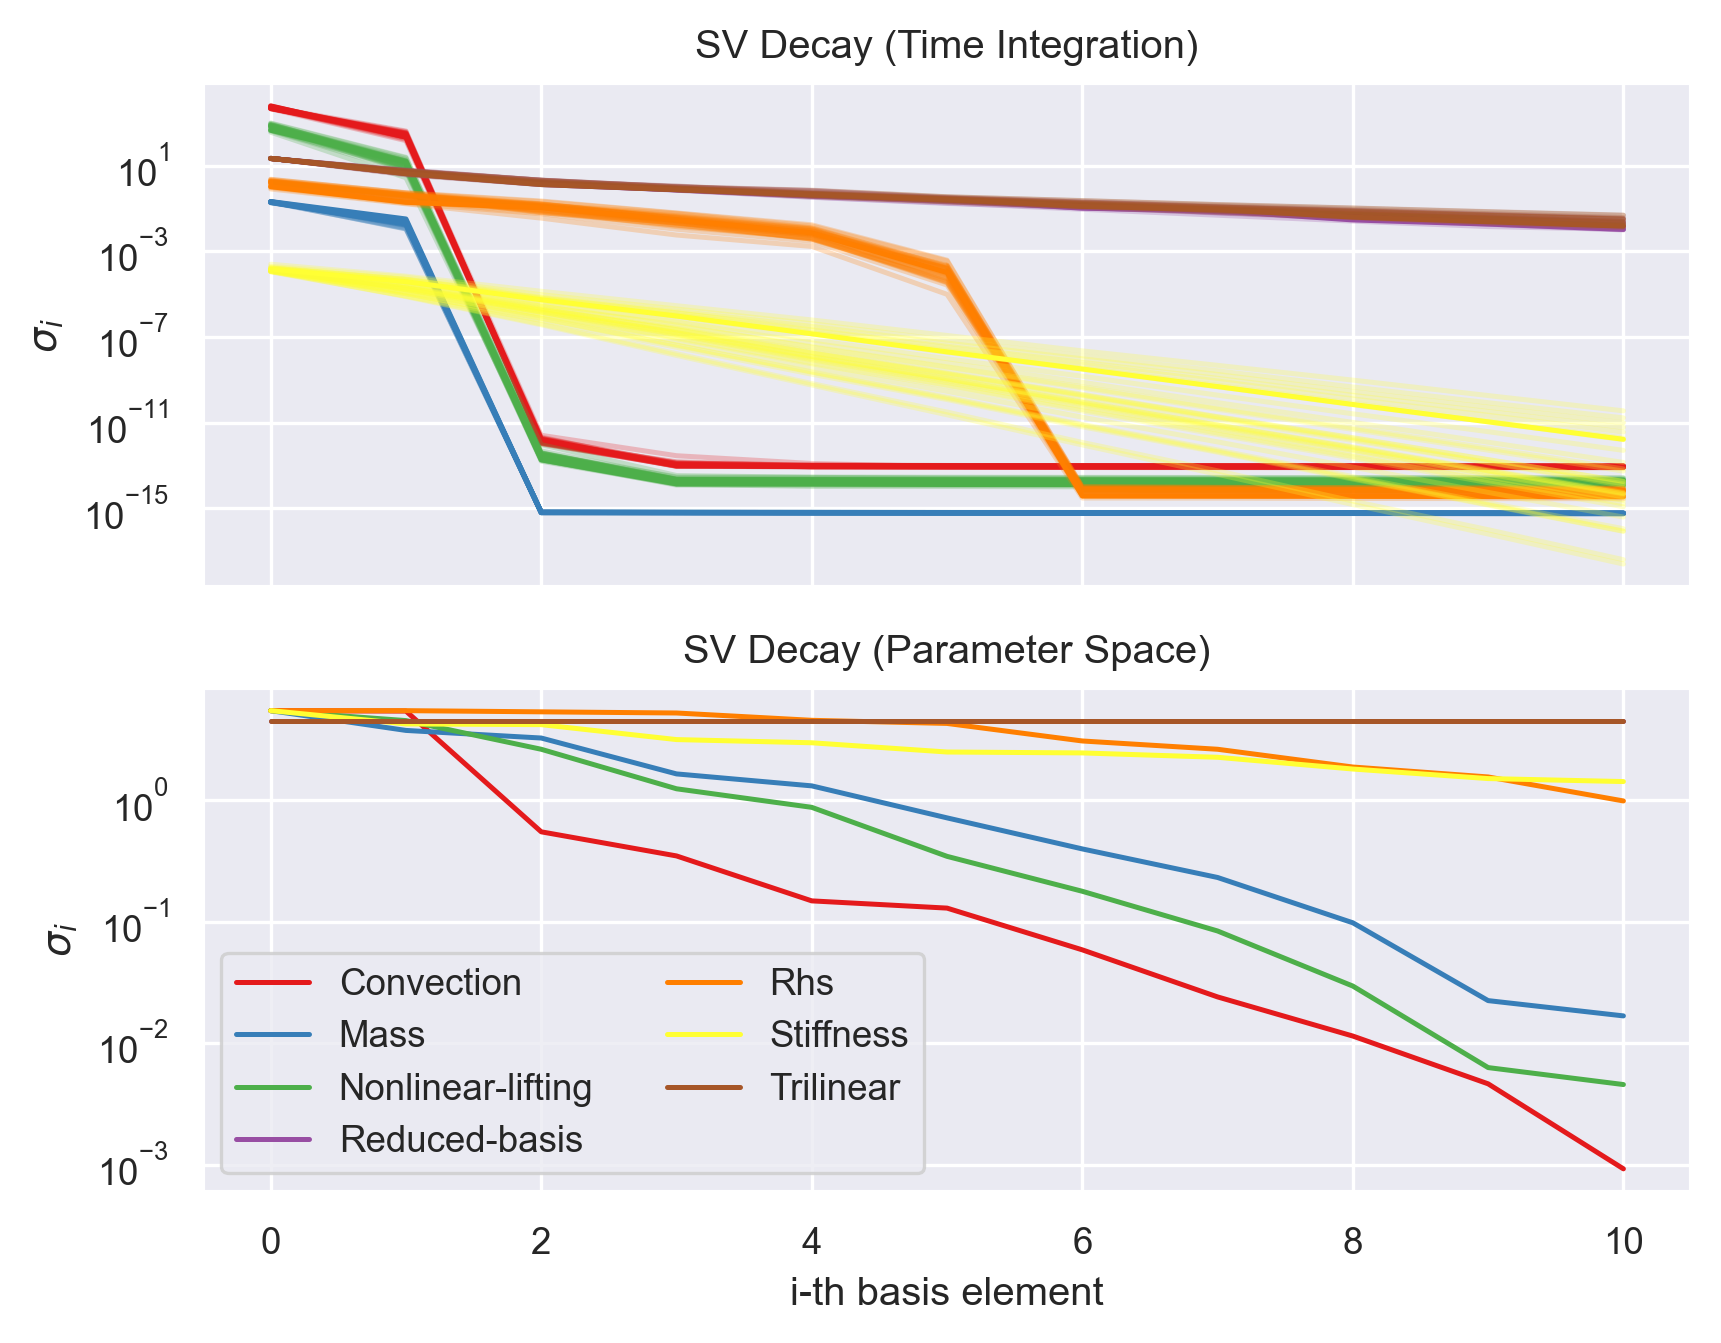
\includegraphics[width =\columnwidth]{research_project/piston/figures/nonlinear_displacement/separable/sigmas_logy.png}
    \caption{This figure is a zoom-in of Figure~\ref{fig:nlinear_disp_sep_loglog}.
    Only the first ten singular values (modes) are shown.
    We can see how for the time integration step most operators 
    are perfectly summarized with two to six modes.
    This is due to the fact that the displacement is separable in time and space;
    and only the space function is not linear.}
    \label{fig:nlinear_disp_sep_logy}
\end{figure}

\begin{figure}[h]
    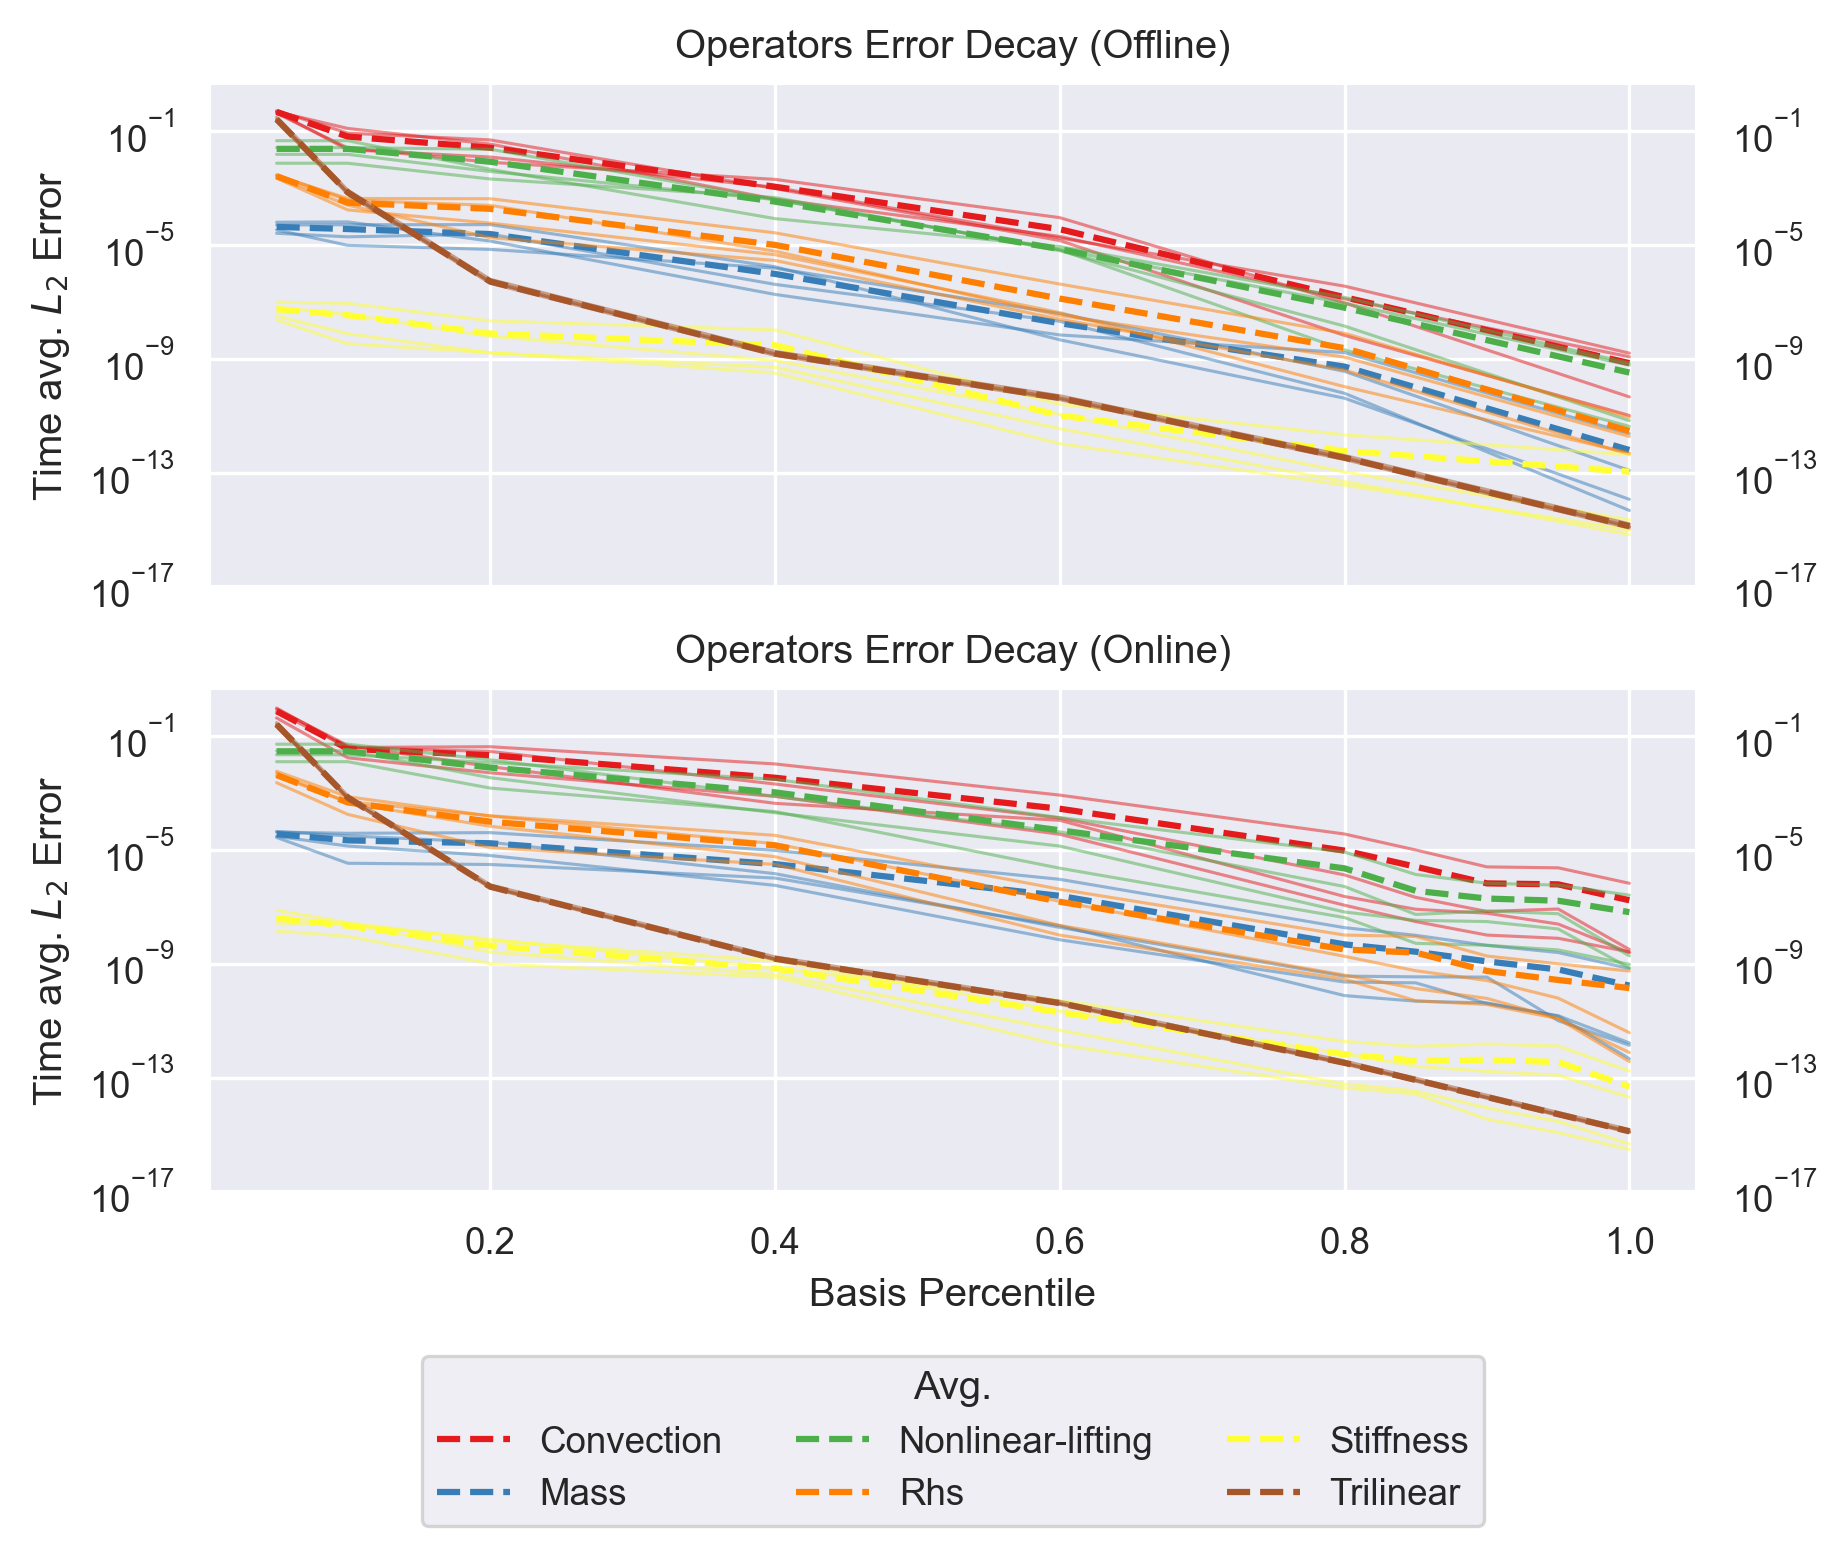
\includegraphics[width =\columnwidth]{research_project/piston/figures/nonlinear_displacement/separable/operators_error_decay_percentile.png}
    \caption{Operator error decay as a function of basis size percentile. \\
    (Top) Offline parameter sample.
    (Bottom) Online parameter sample.
    All the errors decay as the basis size increases, 
    but each operator needs a different basis size to reach the same error threshold.
    For the offline samples, the errors are concentrated.
    For the online samples, the errors present more dispersion.
    The errors with the full basis are smaller for the offline pool, 
    compared to those from the online pool.
    This is an expected behaviour, 
    since the basis is optimized for the offline sample.}
    \label{fig:nlinear_disp_operators_error_decay}
\end{figure}

\newpage
\subsection{Certification by Truncation: Limits}
\label{sec:certification_limits}
We already saw in the heatmap from Figure~\ref{fig:nonlinear_error_decay_heatmap}
in Section~\ref{sec:reduced_basis_mdeim_error_interaction}
how the RB and MDEIM approximation errors could 
set a lower bound to the HROM error.
We show how this interaction can make 
the HROM certification by truncation fail.
\begin{table}[h]
    \centering
    \caption{Online parametrization.
    The results will only be obtained for one parameter,
    since the conclusions scale for many.}
    \begin{tabular}{ccc}
    \toprule
        Variable   & Value  \\ 
        \midrule
        $a_0$      & 18.64   \\
        $\omega$   & 24.78   \\
        $\delta$   & 0.28    \\
        $u_p$      & 0.37    \\
        \midrule
        $x_c$      & 0.32    \\
        $\sigma_c$ & 0.14    \\
        $y_c$      & 0.26    \\ 
        \bottomrule
    \end{tabular}
    \label{tab:parameters_online_arbitrary}
\end{table}
To do so, we set the experiments shown in 
Tables~\ref{tab:certification_experiments_grid} 
and~\ref{tab:certification_experiments_results}.
The online parametrization is given in Table~\ref{tab:parameters_online_arbitrary}.
We want to determine the error estimator behaviour when 
the RB solution approximation error is smaller or greater than the (M)DEIM error.

The conclusion of the experiments is that if the RB solution error 
is smaller than the (M)DEIM error,
the HROM error is saturated by the (M)DEIM errors;
and hence the model truncation technique cannot be used to certify the HROM results,
because both HROMs produce the same result.
When the RB solution error is greater than the (M)DEIM error, 
the trucation technique will produce effective error estimations.

\begin{table}[h]
    \centering
    \caption{Numerical experiments configuration. 
    Pure ROM means no (M)DEIM is used.
    HROM means all collateral bases are used.}
    \begin{tabular}{ccc}
        \toprule                                                           
        & Pure ROM & HROM \\ 
        \midrule                                                           
        $\varepsilon_{\text{RB}}$ > $\varepsilon_{\text{MDEIM}}$ & Figure~\ref{fig:nlinear_disp_no_deim_errors_above_threshold} & Figure~\ref{fig:nlinear_disp_deim_errors_above_threshold}     \\
        $\varepsilon_{\text{RB}}$ < $\varepsilon_{\text{MDEIM}}$ & Figure~\ref{fig:nlinear_disp_no_deim_errors_below_threshold} & Figure~\ref{fig:nlinear_disp_deim_errors_below_threshold} \\
        \bottomrule
    \end{tabular}    
    \label{tab:certification_experiments_grid}
\end{table}
\begin{table}[h]
    \centering
    \caption{Numerical experiments summary.
    The bases size and the order of magnitude of the error are provided.}
    \begin{tabular}{ccccc}
        \toprule
        Experiment                                                   & (M)DEIM    & ROM         & SROM       & Estimator \\
        {}                                                           & {}         & $N$, Error  & $N$, Error & {}         \\
        \midrule
        Figure~\ref{fig:nlinear_disp_no_deim_errors_above_threshold} &  -         &  $15 , 10^{-4}$  & $25 , 10^{-6}$ & Accurate  \\
        Figure~\ref{fig:nlinear_disp_no_deim_errors_below_threshold} &  -         &  $25 , 10^{-6}$  & $30 , 10^{-7}$ & Accurate  \\
        Figure~\ref{fig:nlinear_disp_deim_errors_above_threshold}    &  $10^{-6}$ &  $15 , 10^{-3}$  & $25 , 10^{-4}$ & Regular  \\
        Figure~\ref{fig:nlinear_disp_deim_errors_below_threshold}    &  $10^{-6}$ &  $25 , 10^{-4}$  & $30 , 10^{-4}$ & Ineffective \\
        \bottomrule
    \end{tabular}
    \label{tab:certification_experiments_results}
\end{table}

\clearpage
\begin{figure}[h]
    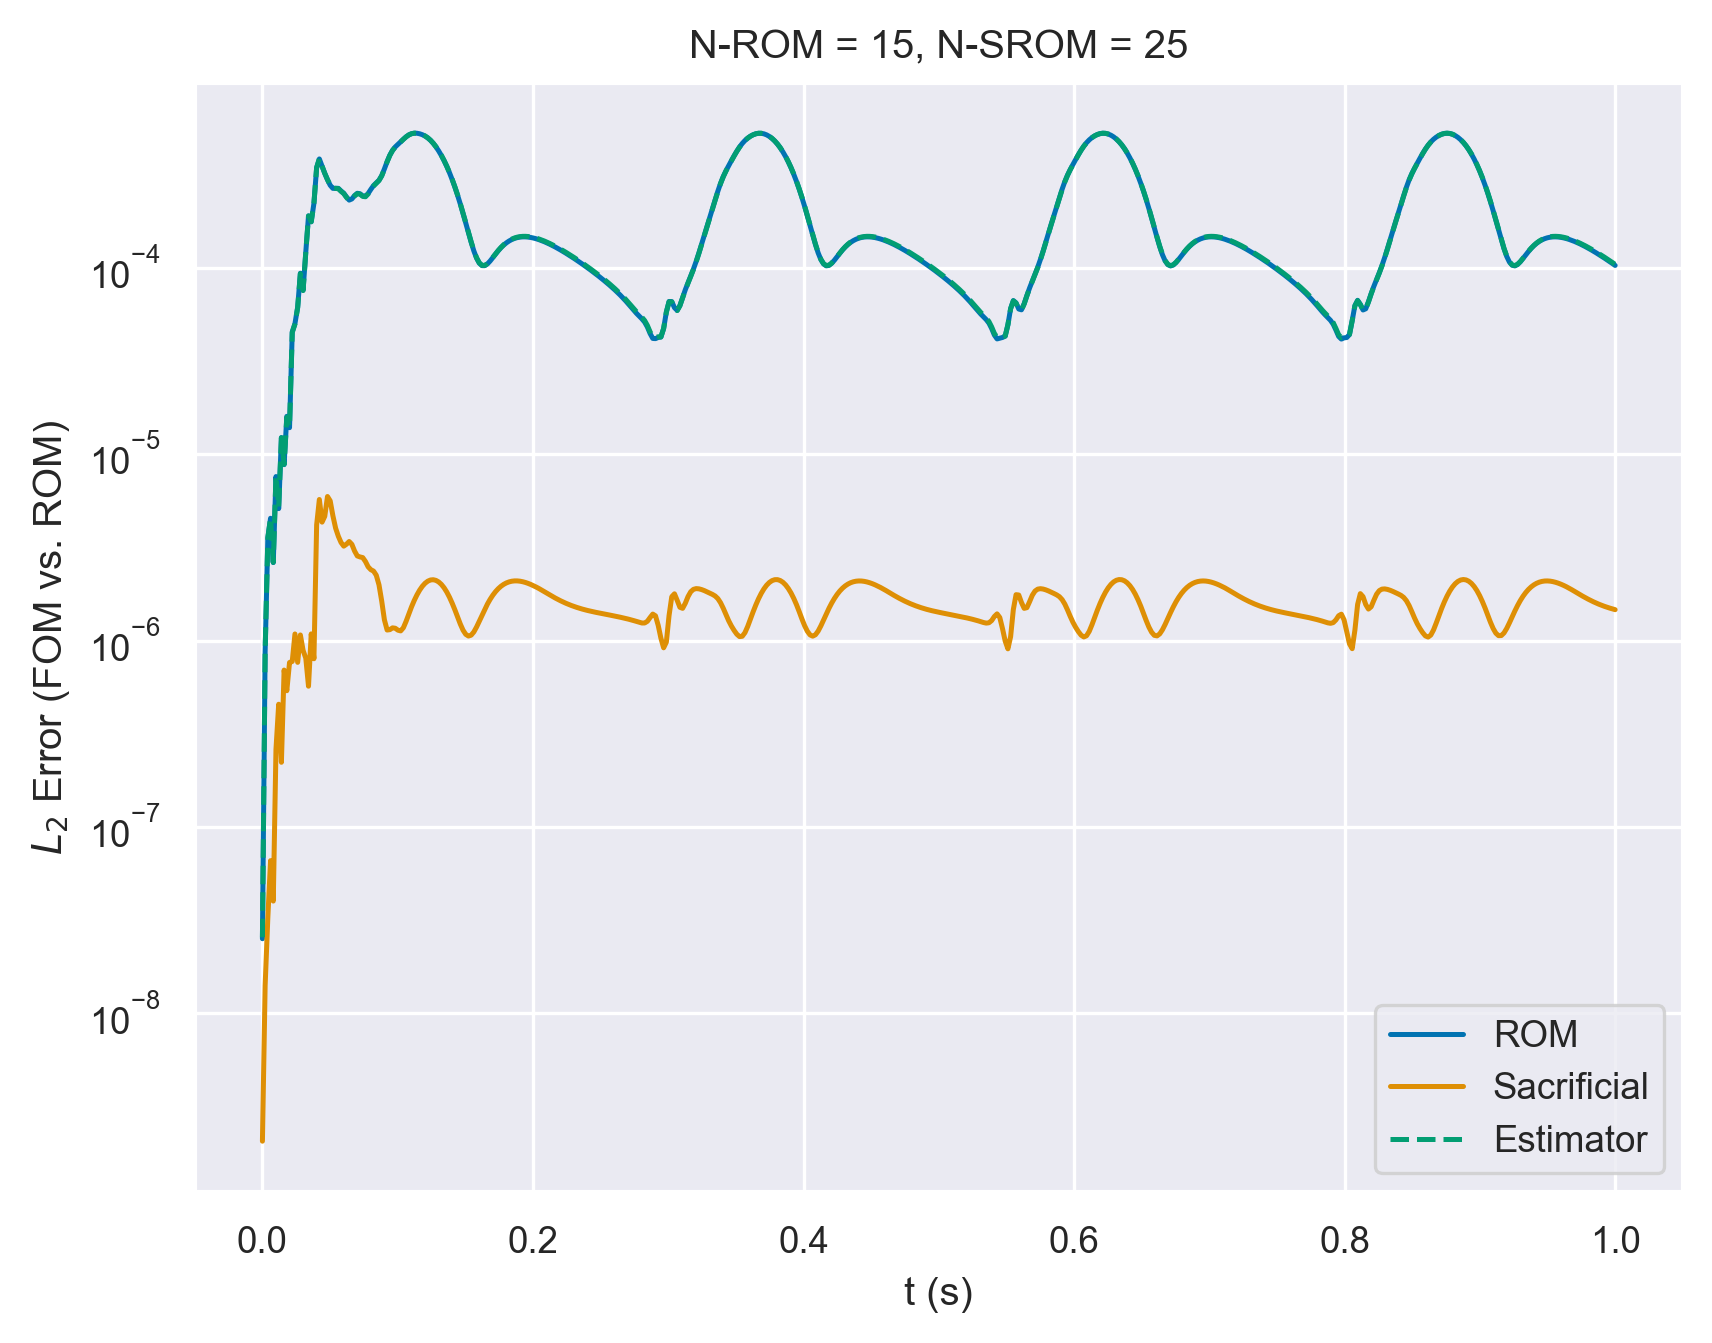
\includegraphics[width =\columnwidth]{research_project/piston/figures/nonlinear_displacement/truncation_error/no_deim/error_estimation_rom_15_srom_25_0.png}
    \caption{ROM vs. FOM approximation error, no (M)DEIM.
    The FOM operators are assembled and projected for each time step.
    The certification by truncation procedure is accurate, with the estimator matching the ROM error.}
    \label{fig:nlinear_disp_no_deim_errors_above_threshold}
\end{figure}

\begin{figure}[h]
    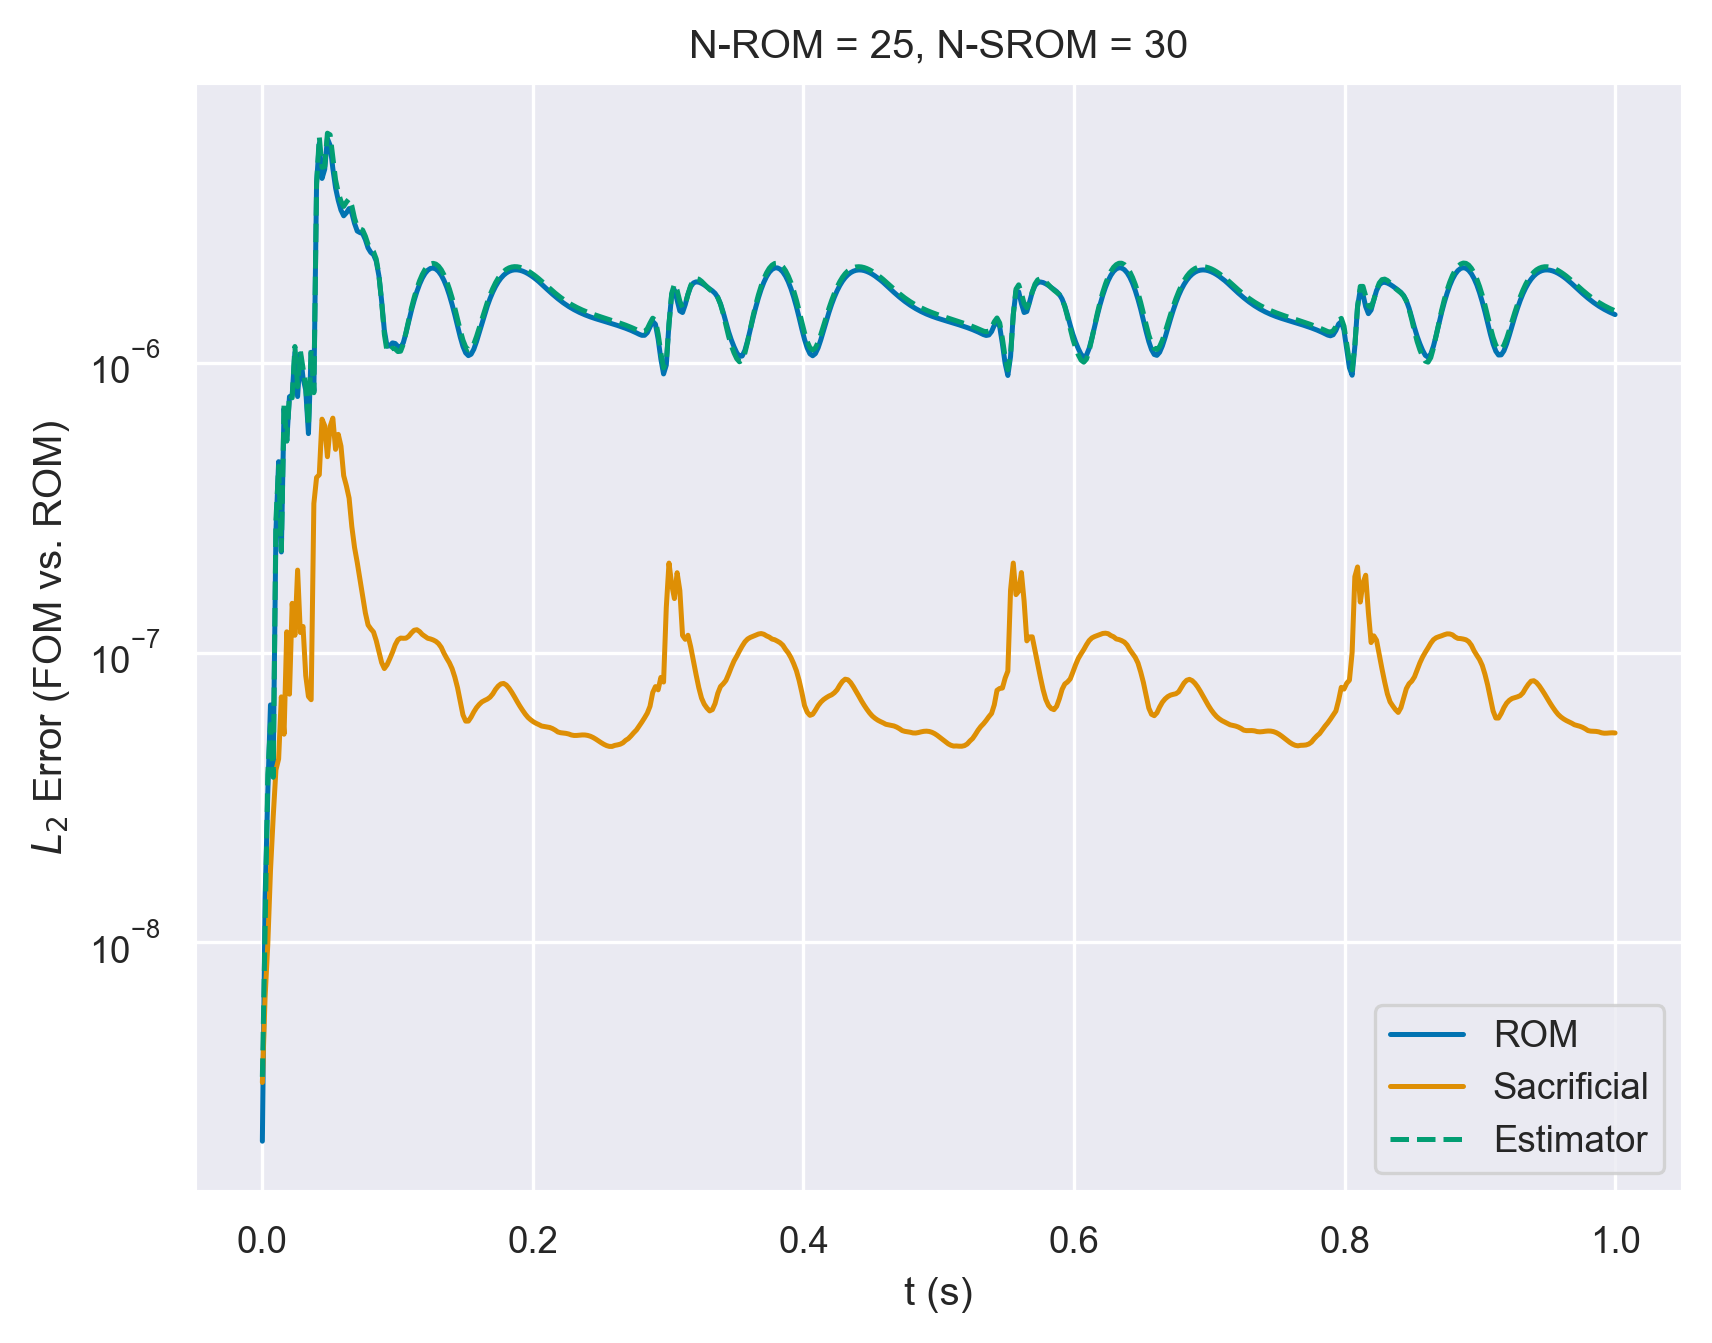
\includegraphics[width =\columnwidth]{research_project/piston/figures/nonlinear_displacement/truncation_error/no_deim/error_estimation_rom_25_srom_30_0.png}
    \caption{ROM vs. FOM approximation error, no (M)DEIM.
    The FOM operators are assembled and projected for each time step.
    The certification-by-truncation procedure is accurate, 
    with the estimator matching the ROM error.}
    \label{fig:nlinear_disp_no_deim_errors_below_threshold}
\end{figure}

\newpage
\begin{figure}[h]
    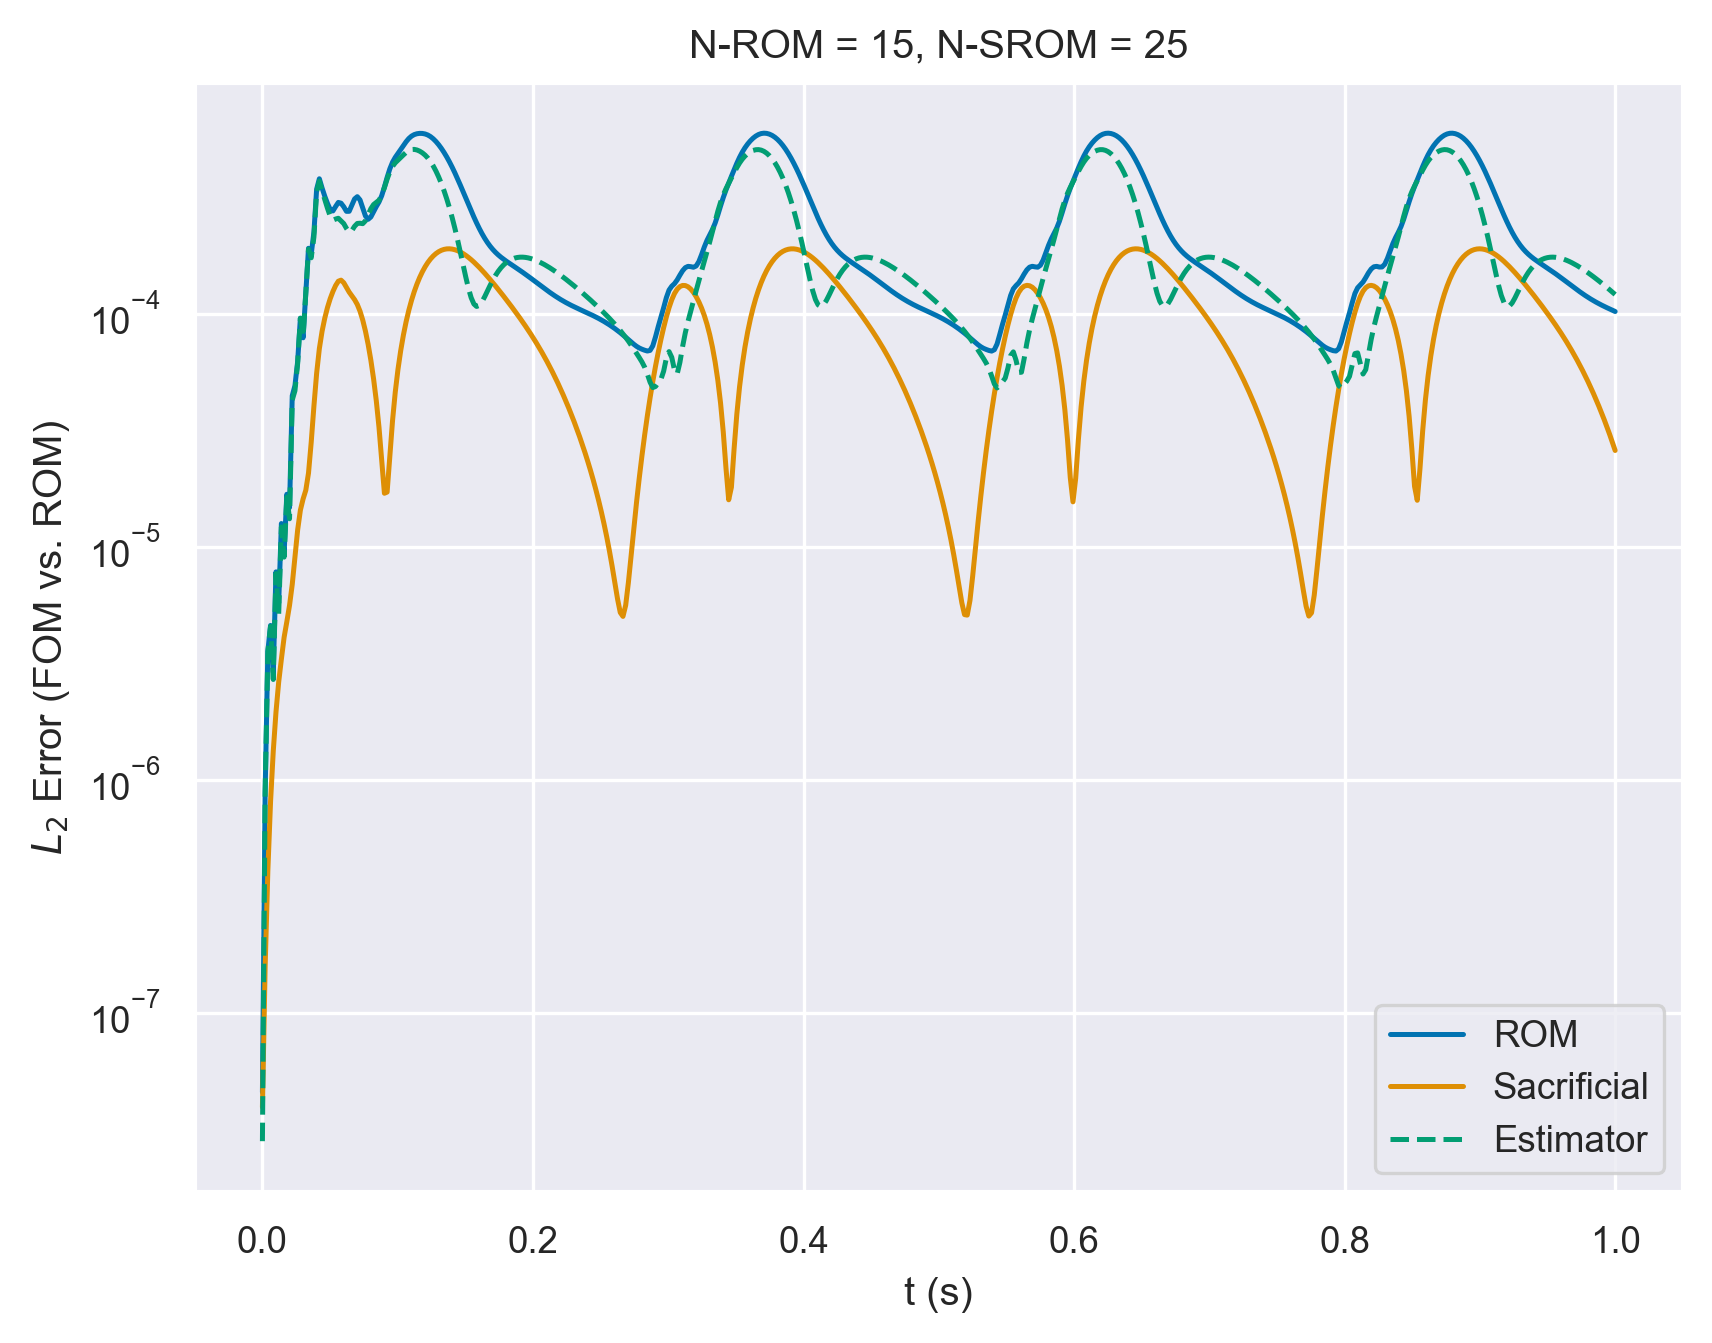
\includegraphics[width =\columnwidth]{research_project/piston/figures/nonlinear_displacement/truncation_error/deim/error_estimation_rom_15_srom_25_0.png}
    \caption{ROM vs. FOM approximation error, (M)DEIM is active.
    The approximation error for all operators is $10^{-6}$.
    The error of the SROM has increased, but it remains smaller than the ROM error.
    Hence, the certification-by-truncation procedure produces a valid estimator.
    % (although not as sharp as when no (M)DEIM is activated, 
    % see Figure~\ref{fig:nlinear_disp_no_deim_errors_below_threshold}).
    }
    \label{fig:nlinear_disp_deim_errors_above_threshold}
\end{figure}

\begin{figure}[h]
    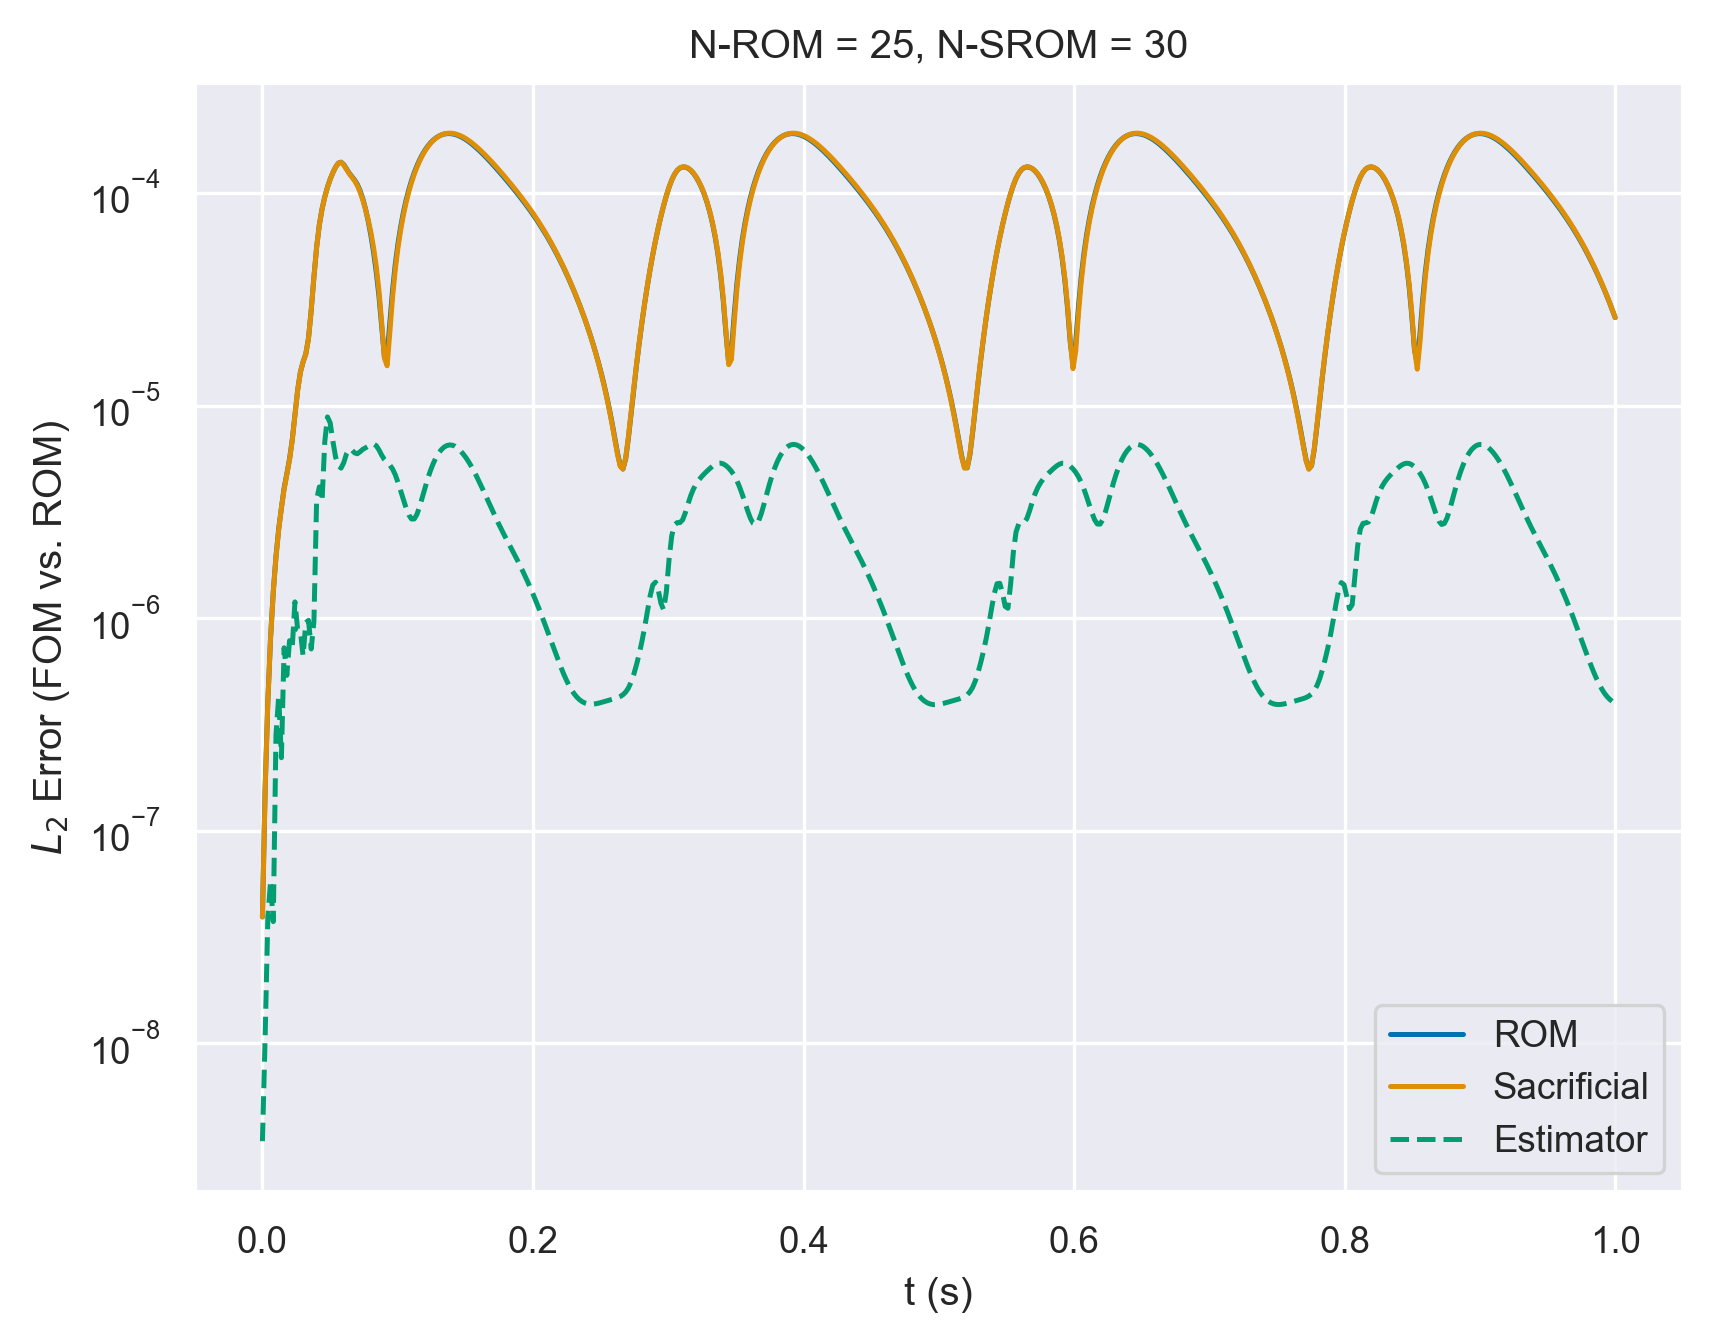
\includegraphics[width =\columnwidth]{research_project/piston/figures/nonlinear_displacement/truncation_error/deim/error_estimation_rom_25_srom_30_0.png}
    \caption{ROM vs. FOM approximation error, (M)DEIM is active.
    The approximation error for all operators is $10^{-6}$.
    The error for the ROM and the SROM is the same, leading to an ineffective truncation estimator.}
    \label{fig:nlinear_disp_deim_errors_below_threshold}
\end{figure}

\clearpage
\subsection{Non-Uniform Mesh: Restricted N-MDEIM}
\label{sec:arbitrary_mesh_nmdeim_mode_evaluation}
In this final section we build the N-MDEIM basis for the trilinear term
from snapshots obtained from RB solution modes evaluation 
($u^{*}$-restricted).

We anticipate that we obtain a non-hierarchical basis as in
Section~\ref{sec:nmdeim_one_mode} 
(\nameref{sec:nmdeim_one_mode}), 
despite the non-uniform spacing of the mesh.
This is due to the following facts:
\begin{itemize}
    \item The domain is one-dimensional.
    \item The FEM basis functions are $\mathbb{P}1$ polynomials.
    \item The trilinear integrand is linear in all of its arguments (including parameters).
    \item The trilinear integrand contains one derivative (trial function $u$).
\end{itemize}
The last fact is crucial, making the non-uniform mesh size go unnoticed.
For $\mathbb{P}1$ polynomials, the derivative of the Lagrangian function 
is the inverse of the mesh size, which gets cancelled by the integration.
This is a known fact of convection-like forms, 
for which the mesh size does not show up in the FEM matrix.
We could have expected that due to the non-uniform displacement,
the mesh size would have an impact in the matrix elements.
However, in the specific context described in the list above,
this is not the case.
For our particular scenario 
(despite the the non-uniform of the mesh displacement),
to reduce the trilinear form it is sufficient to collect snapshots for one parameter
for as many RB solution modes as we will be using for the HROM simulation
(taking into account the SROM). 

As we saw in previous sections, when the basis is not hierarchical, 
the reconstruction error cannot be used as a proxy to determine the accuracy of the collateral basis.
Our conclusion here is that for this trilinear form, 
the collateral basis error will be as good as the error associated 
to the RB solution basis used to assemble the snapshots.

This is shown in Figure~\ref{fig:nlinear_disp_modes_5_rom_15}.
The \mbox{N-(M)DEIM} has been assembled with the first five RB solution modes.
In comparison to the results in Figure~\ref{fig:nlinear_disp_no_deim_errors_above_threshold},
which only reflect the RB solution error\footnote
{
    We recall that no (M)DEIM is active there.
};
these HROMs underperform because the \mbox{N-MDEIM} captures the dynamics for the first five RB solution modes,
where the ROM and the SROM have 15 and 25 respectively.
Instead, when the \mbox{N-MDEIM} is assembled with 15 modes, the ROM recovers its original accuracy,
see Figure~\ref{fig:nlinear_disp_modes_15_rom_15}.

Furthermore, since the SVD creates a linear combination of the inputs;
for non-hierarchical operator bases, trucating the RB operator basis is 
not equivalent to collecting the snapshots without the same number of removed RB solution modes.

\newpage
\begin{figure}[h]
    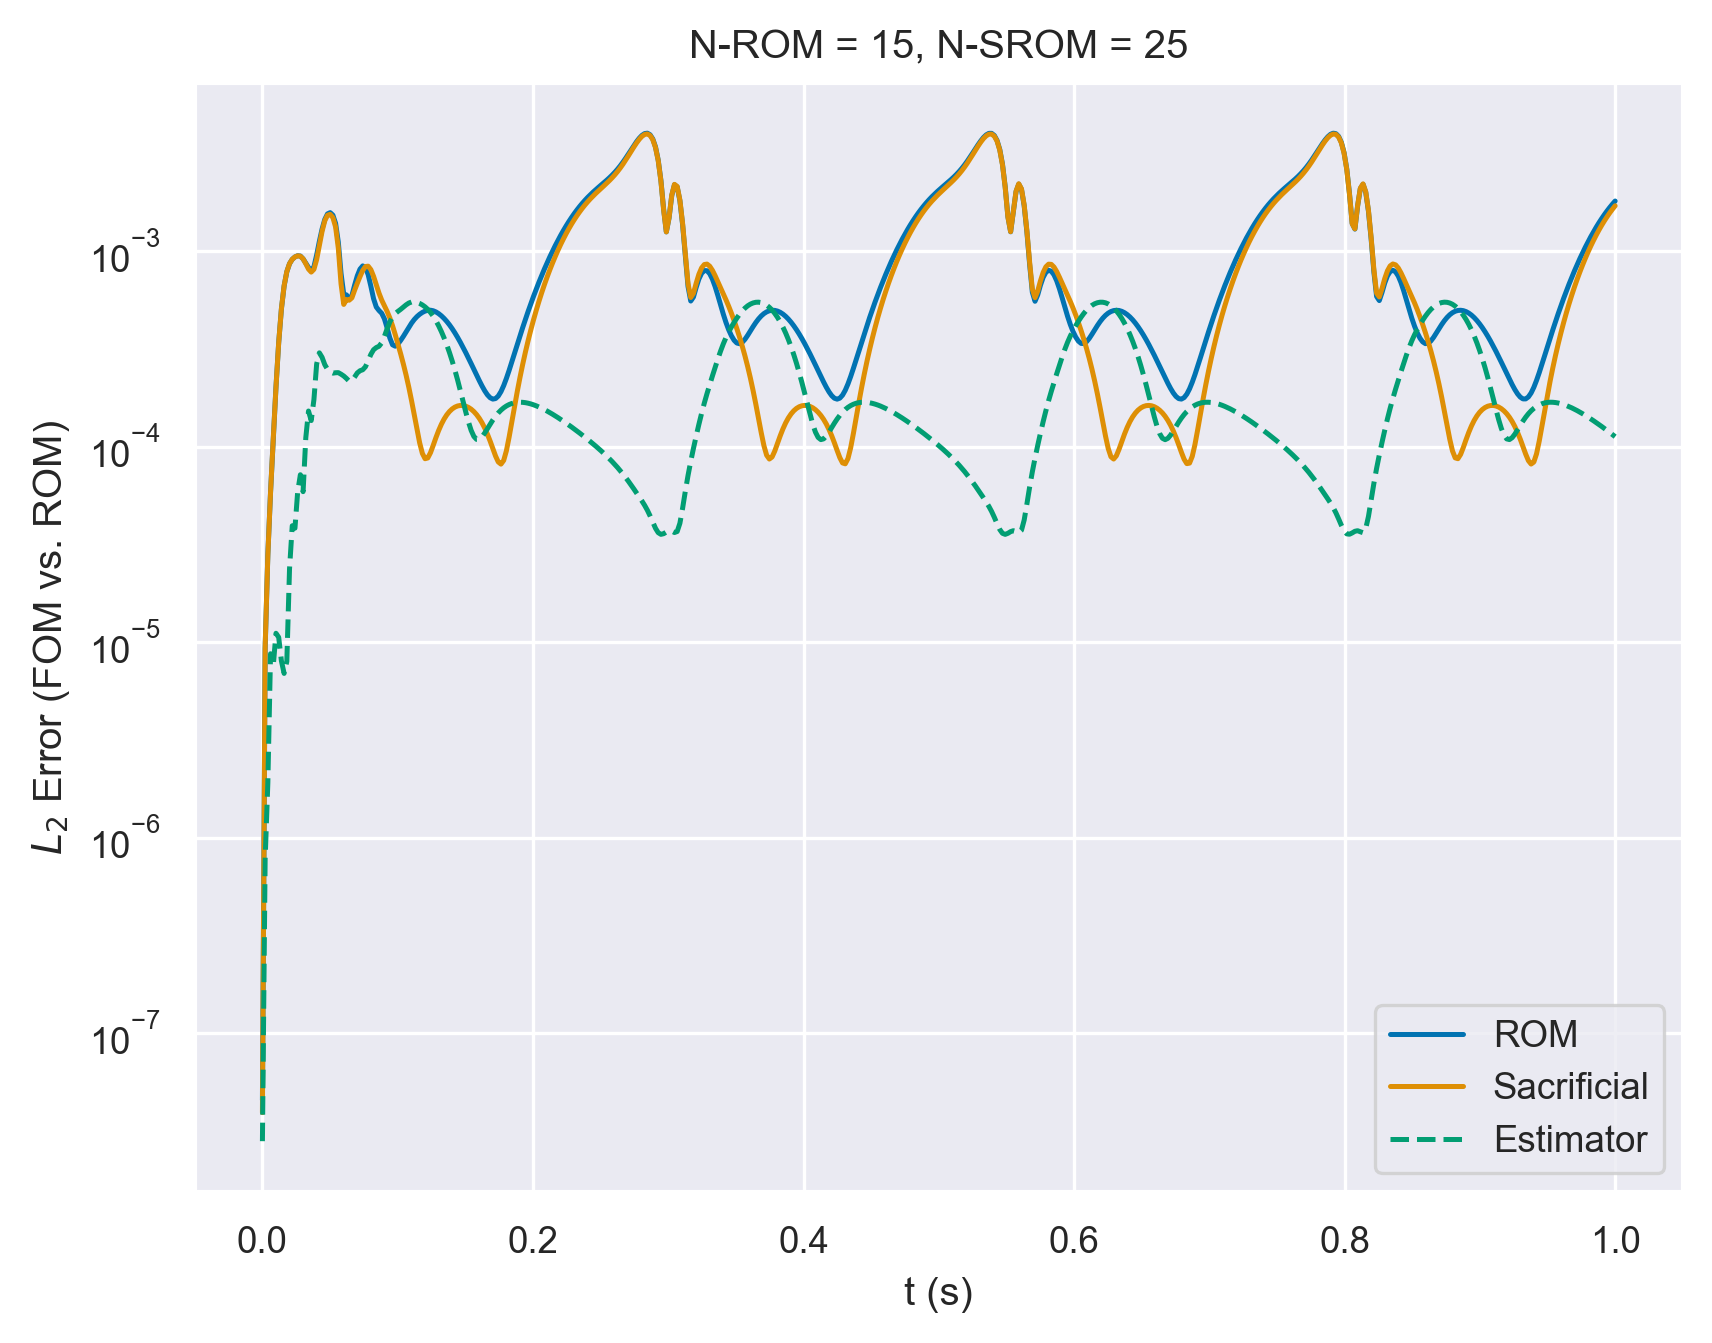
\includegraphics[width =\columnwidth]{research_project/piston/figures/nonlinear_displacement/arbitrary/error_estimation_rom_15_srom_25_modes_5.png}
    \caption{ROM vs. FOM approximation error.
    The (M)DEIM bases size for the linear operators is such that the error is $10^{-6}$.
    The trilinear N-MDEIM has been assembled with $N=5$ RB solution modes.
    The ROM and the SROM are poorly resolved due to unsufficient representation of the excess
    modes they carry with respect to the N-MDEIM training modes.}
    \label{fig:nlinear_disp_modes_5_rom_15}
\end{figure}
\begin{figure}[h]
    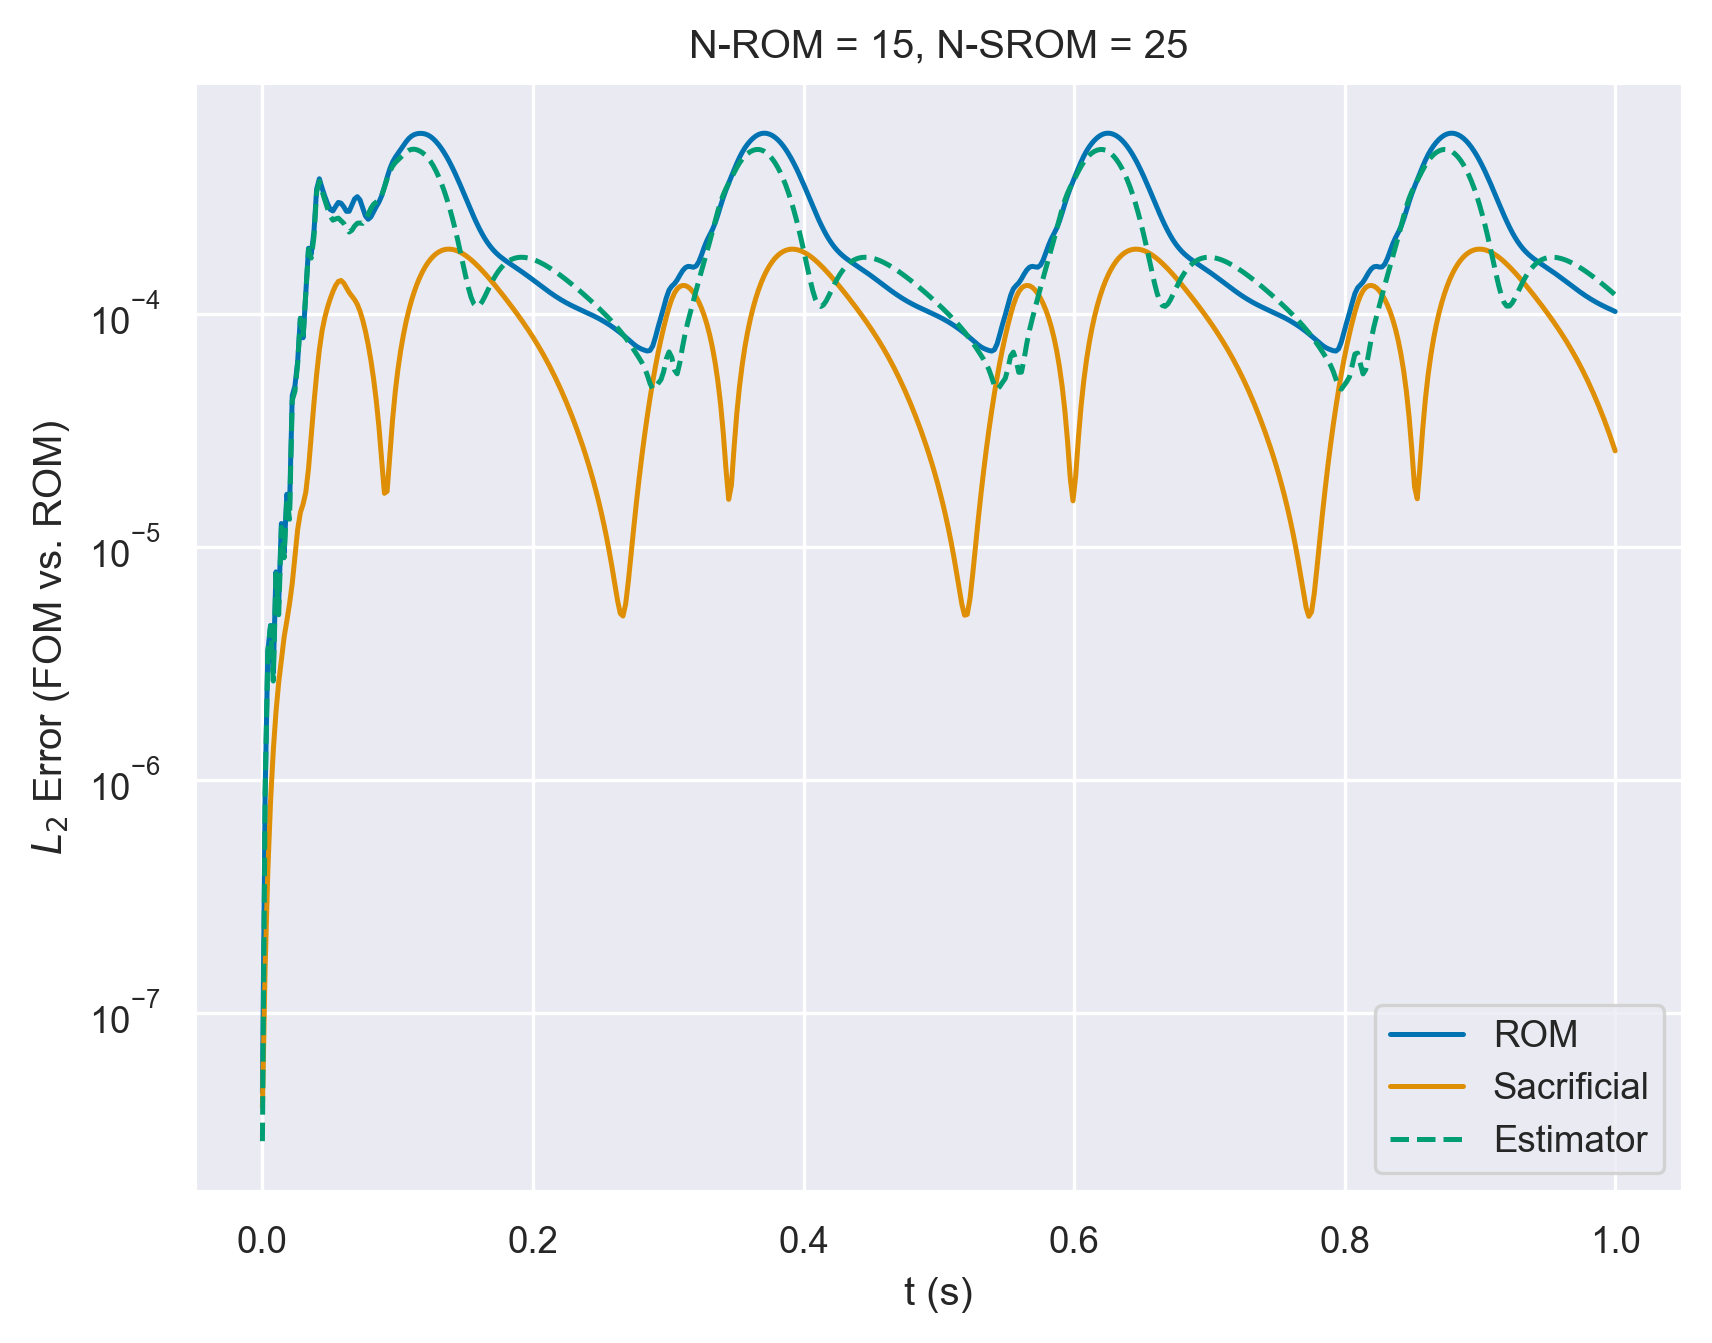
\includegraphics[width =\columnwidth]{research_project/piston/figures/nonlinear_displacement/arbitrary/error_estimation_rom_15_srom_25_modes_15.png}
    \caption{ROM vs. FOM approximation error.
    The (M)DEIM bases size for the linear operators is such that the error is $10^{-6}$.
    The trilinear N-MDEIM has been assembled with $N=15$ RB solution modes. 
    The ROM recovers its original accuracy, since the N-MDEIM is accurately represented for 
    that number of modes.
    Instead, the SROM presents a larger error than expected, 
    due to the excess RB solution modes it carries with respect to the N-MDEIM training modes.}
    \label{fig:nlinear_disp_modes_15_rom_15}
\end{figure}

\end{document}